% Template to be used while publishing    
% a scientific work (PhD Thesis etc.)
% at the EDOC-Server of HU-Berlin                      
%    developed 2003-2008 by
% AG Elektronisches Publizieren, 
% Computer- und Medienservice,
% Humboldt-Universitaet zu Berlin
%    with friendly support of
% TeX-Stammtisch in Berlin     

% $Revision: 19 $
% $HeadURL: svn+ssh://ryckojox@svn.cms.hu-berlin.de/svn/projects/epub/latex/hudiss/mustermann.tex $
% $Date: 2009-07-03 15:49:19 +0200 (ptk, 03 lip 2009) $
% $Author$
% $Id: mustermann.tex 19 2009-07-03 13:49:19Z ryckojox $
                             
% Questions, comments, support:
%    edoc-latex@cms.hu-berlin.de    

% Documentation and information about the conditions of a publication:
%    http://edoc.hu-berlin.de/e_autoren/latex          

% Upload:
%    https://edoc.hu-berlin.de/cgi/dokupload/dokupload.cgi

\documentclass[openright,11pt% 
]{scrbook}[2007/12/24]

\usepackage{textcomp}
%\usepackage[english,ngerman]{babel}
%\usepackage[CaptionAfterwards]{fltpage}
% The following package is necessary.
% To change the default options of the packages, use the key=value interface.
% See the documentation for details.
% If you need to use any special characters or LaTeX-commands 
% within the options, use \hudisssetup{} after loading this package,
% otherwise they will NOT work correctly.
\usepackage[    
    inputenc=utf8, % default - latin1, utf8
    % fontset=palatino, % other possible parameters: lmodern, times
    % natbib={}, %include to use the natbib-package
    % jurabib={}, %include to use the jurabib-package
    % apacite={}, %include to use the apacite-package
    hints=false, % set to 'false' for submission
    checktabu=false, % set to 'false' for submission
    draft=false, % set to 'false' for submission
    qserie=false
 ]{hudiss}
% 2013 Oct by JHS: hudiss has been patched to account for edoc demands
% the geometry package was used to adjust margins. This only works for
% the default A4 setting. A5 (wich would be allowed as well) has not
% been tested - sorry.
               
\hudisssetup{%
    titlepagefont={\Large\sffamily} % Use to change the titlepage font
}

\makeatletter
\renewcommand{\fnum@figure}{Figure \thefigure}
\makeatother

% Fill out all the metadata here:
\hudissmetadata{%
    authorprefix={M.Sc.}, % e.g. Dipl.-Inf.
    authorfirstname={Nikolay Aleksandrov}, % first name
    authorsurname={Chenkov}, % surname
    authorsuffix={\!}, % e.g. Ph.D.
    %authoradd={gebohren in XXX}, % date and place of birth
    doctitle={Mechanisms behind sharp-wave ripple generation}, % title of the thesis
    docsubtitle={xxx}, % subtitle of the thesis
    % docsubject={}, % subject of the thesis (used in the properties of the pdf-document)
    % approvala={................................}, % 
    % approvalb={................................},
    % approvalc={................................},
    approvala={Richard Kempter}, % during first submission use dots!
    approvalb={Reviewer B},
    approvalc={Reviewer C},
    % approvald={},
    % approvale={},
    degree={d\,o\,c\,t\,o\,r\;\;r\,e\,r\,u\,m\;\;n\,a\,t\,u\,r\,a\,l\,i\,u\,m\\(Dr. rer. nat.)},
    subject={Theoretische Biologie}, % e.g. Informatik
    faculty={Mathematisch-Naturwissenschaftlichen Fakult\"at I}, % in Dativ/Genitiv! e.g. Mathematisch-Wissenschaftlichen Fakult\"at II
    university={Humboldt-Universit\"at zu Berlin}, % e.g. Humboldt-Universit\"at zu Berlin
    dean={Prof. Stefan Hecht, PhD}, % dean of the faculty
    president={Prof. Dr. Jan-Hendrik Obertz}, % president of the university
    datesubmitted={20.09.2012}, % the date of the submission
    %dateexam={08.04.2013}, % the date of your last exam
    %keywordsen not working
    keywordsen={assembly, sequence, replay, sharp-wave ripple, memory}, % english keywords comma separated
    %keywordsde={Kanalrauschen, ...} % german keywords comma separated
}

% If you whish to load any further packages, 
% make any own adjustments (e. g. for the package fancyhdr)
% or define any own commands
% put ALL of them in the following file:
%%%%%%%%%%%%%%%%%%%%%%%%%%%%
% Load additional packages %
%%%%%%%%%%%%%%%%%%%%%%%%%%%%

% use pdf or images
\newcommand{\usepdfpics}{1}

% Bibliography
\usepackage[round]{natbib} %was[numbers]
% Math packages and example envoronment
\usepackage{amsmath,amssymb,amsfonts}
\usepackage{amsthm}
\usepackage{thmtools}
\usepackage{algorithmic}
%\usepackage{esint}
% \DeclareMathAlphabet{\mathscr}{OT1}{pzc}%
%                                  {m}{it}
%\usepackage[utopia]{mathdesign}
%\usepackage[OMLmathrm,OMLmathbf]{isomath}
%\usepackage{mathabx} % creates nicer integral symbols
\usepackage{tocstyle} % needed to adjust spacing betwen toc number and title
\usetocstyle{standard}
% this one is too fancy?
% \usepackage{titletoc}
% \titlecontents{chapter}[1.5em]{\addvspace{1pc}\bfseries}{\contentslabel{5em}}{}
%     {\titlerule*[0.3pc]{.}\contentspage}
\usepackage{upgreek}
\usepackage{mathrsfs}
\usepackage{mathtools}
\usepackage{bbm}
\usepackage{makeidx}
\makeindex
\usepackage{appendix} % removes appendix numbering?
\usepackage[small]{caption}

%%%%%%%%%%%%%%%%%%%%%
% added by klesk NC %
%%%%%%%%%%%%%%%%%%%%%
\usepackage{verbatim}
\graphicspath{{figs/}}

\makeatletter
\renewcommand{\fnum@figure}{Figure \thefigure}
\makeatother

%%%%%%%%%%%%%%%%%%%%%%%%%%%%%%%%%
% Add special math environments %
%%%%%%%%%%%%%%%%%%%%%%%%%%%%%%%%%
% \theoremstyle{definition}
% \newtheorem{example}{Example}
\declaretheorem[style=definition]{example}

%\renewcommand\thmcontinues[1]{Continued}

%%%%%%%%%%%%%%%%%%%%%%%%%%%%%%
% Redefine section headdings %
%%%%%%%%%%%%%%%%%%%%%%%%%%%%%%


% section easier to reference with \S
% \renewcommand{\thechapter}{\arabic{chapter}\rm}
%\renewcommand{\thesection}{\S\arabic{chapter}.\arabic{section}\rm}
%\renewcommand{\thesubsection}{\S\arabic{chapter}.\arabic{section}.\arabic{subsection}}
%\renewcommand{\thesubsubsection}{\Roman{subsubsection}}
% \makeatletter
%   \renewcommand\l@subsection{\@dottedtocline{2}{1.5em}{8em}}
% \makeatother

%\renewcommand{\captionfont}{\small\slshape}
%%%%%%%%%%%%%%%%%%%%%%%%%%%%%%%
% Adjust figure caption style %
%%%%%%%%%%%%%%%%%%%%%%%%%%%%%%%

% English caption label and font size changed
\addto\captionsenglish{% 
  \renewcommand{\figurename}{Fig.} 
  % does not work 
  %\renewcommand{\captionfont}{\small} 
}
% \captionnamefont{\bfseries}
% \captiontitlefont{\small} 


% indenting
\parindent0ex

\addtokomafont{disposition}{\rmfamily} 
\addtokomafont{title}{\rmfamily}

% set all math to small symbols (saving space)
%\everymath={\textstyle}
%\DeclareMathSizes{display size}{text size}{script size}{scriptscript size}.
\everymath=\expandafter{\the\everymath\textstyle}

%%%%%%%%%%%%%%%%%%%%%%%%%%%
% provide custom commands %
%%%%%%%%%%%%%%%%%%%%%%%%%%%
\newcommand{\bra}{\langle}
\newcommand{\cv}{\boldsymbol}
\newcommand{\chdens}{\varrho}
\newcommand{\dd}{{\mathrm d}}
\newcommand{\fd}{{\updelta}}
\newcommand{\fft}[1]{{\tilde #1}}
\newcommand{\half}{{\textstyle\frac12}}
\newcommand{\imag}{\text{i}}
\newcommand{\ket}{\rangle}
\newcommand{\mtx}{\boldsymbol}
\newcommand{\orbsol}[1]{#1_0}
\newcommand{\pd}{\partial}
\newcommand{\ve}{\varepsilon}
\newcommand{\supzero}{{(0)}}
\newcommand{\supone}{{(1)}}
\newcommand{\suptwo}{{(2)}}
\newcommand{\oth}{{(0)}}
\newcommand{\ith}{{(1)}}
\newcommand{\iith}{{(2)}}
\newcommand{\tAP}{t^\text{AP}}
\newcommand{\tilr}{{\tilde{r}}}
\newcommand{\tils}{{\tilde{s}}}
\newcommand{\tilt}{{\tilde{t}}}
\newcommand{\tp}{{\mathsf{T}}}
\def\updownharpoons{\upharpoonleft\!\downharpoonright}
% some notation
\newcommand{\entropy}{{\mathcal H}}
\newcommand{\fisherI}{\mathcal I}
\newcommand{\fpop}{{\mathcal F}}
\newcommand{\K}{{\text{K}^+}}
\newcommand{\Na}{{\text{Na}^+}}
\newcommand{\Cl}{{\text{Cl}^-}}
\newcommand{\chDiffu}{\mtx D^\mathrm{c}}
\newcommand{\ndim}{d}
\newcommand{\gK}{\bar g_\mathrm{K}}
\newcommand{\gNa}{\bar g_\mathrm{Na}}
\newcommand{\gL}{\bar g_\mathrm{L}}
\newcommand{\EK}{E_\mathrm{K}}
\newcommand{\ENa}{E_\mathrm{Na}}
\newcommand{\EL}{E_\mathrm{L}}
\newcommand{\dcI}{I_\mathrm{DC}}
\newcommand{\nspikes}{{N_\text{sp}}}
\newcommand{\ntrials}{{N_\text{trials}}}
\newcommand{\period}{{T_\text{p}}}
\newcommand{\barperiod}{{\bar T_\text{p}}}
\newcommand{\pot}{\Phi}
\newcommand{\tilZ}{\cv{\tilde Z}}
\newcommand{\str}{y}
\newcommand{\spt}{\tau^{\text{sp}}}
\newcommand{\isi}{\tau^{\text{sp}}}
\newcommand{\orb}{\cv v_0}
\newcommand{\stim}{x}
\newcommand{\rate}{r}
\newcommand{\stdZ}{\cv{\check Z}}
\newcommand{\transinfo}{{\mathcal M}}
% Mathematical operators
\DeclareMathOperator*{\argmin}{argmin}
\DeclareMathOperator{\bn}{Bn}
\DeclareMathOperator{\coh}{coh}
\DeclareMathOperator{\coefvar}{CV}
\DeclareMathOperator{\diag}{diag}
\DeclareMathOperator{\erf}{erf}
\DeclareMathOperator{\mean}{mean}
\DeclareMathOperator{\res}{Res}
\DeclareMathOperator{\sinc}{sinc}
\DeclareMathOperator{\sta}{STA}
\DeclareMathOperator{\stc}{STC}
\DeclareMathOperator{\var}{var}
\DeclareMathOperator*{\tsint}{{\textstyle\int}}
\DeclareMathOperator*{\tssum}{{\textstyle\sum}}
\DeclareMathOperator*{\tsiint}{{\textstyle\iint}}
\DeclareMathOperator*{\rlharp}{\rightleftharpoons}
% English text abreviations
\newcommand{\eg}{{\textit{e.g.}}}
\newcommand{\ie}{{\textit{i.e.}}}
\newcommand{\cf}{{\textit{cf.}}}
\newcommand{\rhs}{r.h.s.}
\newcommand{\viz}{{\textit{viz.}}}
\newcommand{\wrt}{w.r.t.}
\long\def\comment#1{}

% set the language for figures etc
\selectlanguage{english}

% mathfont
\let\oldsum\sum
\renewcommand{\sum}{\mathop{\textstyle\oldsum\limits}}
\let\oldint\int
\renewcommand{\int}{\mathop{\textstyle\oldint\limits}}
\let\oldiint\iint
\renewcommand{\iint}{\mathop{\textstyle\oldiint\limits}}
\let\oldiiint\iiint
\renewcommand{\iiint}{\mathop{\textstyle\oldiiint\limits}}
\let\oldiiiint\iiiint
\renewcommand{\iiiint}{\mathop{\textstyle\oldiiiint\limits}}

% \DeclareMathSizes {t-size} {mt-size} {s-size} {ss-size}
% \DeclareMathSizes{10}{10}{10}{8}
% \renewcommand\displaystyle\textstyle
%\newcommand{\SUM}[2]{\overset{#1}{\underset{#2}{\mathop{\sum}}}}


\newcommand{\lyxline}[1][1pt]{%
  \par\noindent%
  \rule[.5ex]{\linewidth}{#1}\par}

% The order of the parts in the document is only our suggestion,
% you can change it, if you wish.
% Don't put any other text between those commands.
% Do not remove the \*matter macros.
% Use standard macros to include new chapters.
\begin{document}
\setlength{\parindent}{4ex}
\selectlanguage{english}%ngerman
\everymath{\textstyle}
  \frontmatter
    \maketitle
    %\include{dedication}
    \huge\textbf{Abstract}
\normalsize
\vspace{10mm}

blabla in english


\newpage

    \huge\textbf{Zusammenfassung}
\normalsize
\vspace{10mm}

blabla auf Deutsch

\newpage

    \tableofcontents    
  \mainmatter
    \chapter{Introduction}
  \textit{ There is a story that Simonides was dining at the house of a wealthy
    nobleman named Scopas at Crannon in Thessaly, and chanted a lyric poem
    which he had composed in honor of his host, in which he followed the custom
    of the poets by including for decorative purposes a long passage referring
    to Castor and Pollux; whereupon Scopas with excessive meanness told him he
    would pay him half the fee agreed on for the poem, and if he liked he might
    apply for the balance to his sons of Tyndaraus, as they had gone halves in
  the panegyric.  }

  \textit{ The story runs that a little later a message was brought to
    Simonides to go outside, as two young men were standing at the door who
    earnestly requested him to come out; so he rose from his seat and went out,
    and could not see anybody; but in the interval of his absence the roof of
    the hall where Scopas was giving the banquet fell in, crushing Scopas
    himself and his relations underneath the ruins and killing them; and when
    their friends wanted to bury them but were altogether unable to know  them
    apart as they had been completely crushed, the story goes that Simonides
    was enabled by his  recollection of the place in which each of them had
    been reclining at table to identify them for separate interment; and that
    this circumstance suggested to him the \textbf{discovery of the truth that
    the best aid to clearness of memory consists in orderly arrangement}.  }

  \textit{ He inferred that persons desiring \textbf{to train this faculty must
    select localities and form mental images of the facts they wish to
    remember and store those images in the localities, with the result that
    the arrangement of the localities will preserve the order of the facts,
    and the images of the facts will designate the facts themselves}, and we
    shall employ the localities and images respectively as a wax writing tablet
  and the letters written on it.}\footnote{\cite{Cicero}, Book 2, 86.352--54.}\\\\

%\section{Summary}
  This thesis deals with sharp-wave ripples and the associated sequence
  replays. The introduction is intended to give the reader some insight about
  the relevance of these topics to our everyday life. It starts with a brief
  historical overview (Section~\ref{sec:seqs}) on mental sequences and their
  place in the understanding of memory and cognition over the centuries. Then,
  Section~\ref{sec:hebb} dwells into fundamental concepts from Hebb's theory,
  such as synaptic plasticity, neural assemblies, and assembly sequences and
  their implications in theoretical neuroscience. The following
  Section~\ref{sec:hippo} is dedicated to the description the hippocampus and
  its role in memory. Then, Section~\ref{sec:swr} describes the sharp-wave
  ripple phenomenon and the replay of behaviour sequences in a greater detail.

\section{Sequences as a behavioural substrate: a historical overview}
\label{sec:seqs}
  Simonides of Ceos (556--468 BC) was both a celebrated and condemned lyric
  poet in Ancient Greek world. He is famed as the inventor of 4 letters of the
  Greek alphabet ($\eta, \, \psi, \, \xi,\,{\rm and } \,\, \omega$) and is
  considered as the first commercial poet who created songs and odes for pay.
  Moreover, he is in the focus of the oldest reference \citep{Rhetorica} for a
  mnemonic technique called `Method of Loci' or `Memory palace' (see the legend
  above from \cite{Cicero}). The method of loci has survived over the centuries
  as a technique to help orators, artists, clerks, and encyclopedists to
  remember information of virtually any quality and quantity \citep{Yates66}.
  Nowadays, the method takes a central place in the training of every memory
  champion \citep{Foer2011}.
  
  How does this mnemonic technique work? Can a naive person actually remember a
  large list of items consisting of tens or even hundreds of elements? In its
  essence, the method of loci is a mnemonic technique based on images and
  places. To deploy the method, one needs a predefined trajectory in some very
  well known spatial environment (e.g., a good starting point for beginners is
  imagining home). Then, to imprint the list, each item is sequentially placed
  in the virtual trajectory (e.g., entrance door, telephone cupboard,
  bookshelf, door to the living room, sofa, sofa table, etc.) and imagined as
  vividly as possible. It is suggested to recruit as many sensory modalities as
  possible when imagining the placed objects as this creates more hooks for
  later revoke of the items. For the following recall one needs only to do a
  virtual walk through the same trajectory and to recollect the items from
  their places (loci). A vivid imagination is always beneficial for these
  mental exercises.

  %Laura's subject with super memory, having a condition of astasia? has been implementing a similar method, probably unconsciously.. (or a paragraph down?)
  %every super memory human tested so far has been using some memory technique that relies on methos of loci or story
  %creation. Even Luria's subject...colorful memory
  %sequences, tables that could be read by raws, columns and diagonals; after 16 years still remembers
  %using streets from his home town or moscow to place items that has be remembered when given very long lists
  %very strong imagination,  severe synestisia where he feels the color, shape, weight, touch, etc of every word he hears or reads..certain problems in concntration while reading and especially while eating..
  %He never changed items with similar items or with synonims, however, during recall often he could skip some item that was placed in a `dark place' or was not very well distinguished form the background..
  %weak in the logical `organisation of memorizing'
  %bad memory on faces: they are so changeable, changing colors all the time, depending on the mood of the person, on the moment of meet..

  %It is, however, an open question whether the sequential arrangement is an
  %universal quality, or whether some more complex schemata can be used for
  %memory formation and recall. For example, can a two-dimensional pattern be
  %used as a base for the storage of new memories?

  Since ancient times it is known that memory can greatly benefit from
  predefined sequences. All known mnemonic techniques based on the method of
  loci or the story method (e.g., creating a story with the list items to be
  remembered) rely on the sequential storage and the recall of associated
  memories.

  Sequences have been proposed also as a more general model for the occurrence
  and development of the mental processes. The oldest known references to the
  concept of association of thoughts and ideas can be tracked to Plato and
  Aristotle from the ancient world \citep{Plato:Phaedo, Bloch2007}. Later, in
  the western world the thought sequence concept was further developed by early
  modern philosophers \citep{Hobbes, Locke, Hume, Hume2, Stewart}. David
  Hartley, a founder of the associationist school of psychology in the $18^{\rm
  th}$ century, proposed that even the most complex thought processes can be
  explained as sequential activations of clusters of elementary senses and
  representations. At the turn between the $19^{\rm th}$ and the $20^{\rm th}$
  century, a lot of work devoted to associations was contributed in the field
  of psychology: The thought experiment about William James' bear attempts to
  explain the physiological response of the body as sequence of mental events
  after the sensory arousal of seeing a bear \citep{James1884}.
  \cite{Pavlov1897} published his seminal work on the conditioned reflex, where
  he demonstrated the physiological effects of classical conditioning. Further
  work in experimental psychology conceived that sequences of experiences and
  their representations are in the base of motor action, cognition, and
  judgment \citep{Watt1904, Titchener1905, Washburn1916}.

  Various disciplines have looked at the sequences of motor actions, thoughts,
  and memories as a basic behaviour substrate of the human nature. But how are
  such sequences represented in the brain, what is their neural basis?

    %Cajal: neuron doctrine, neurons have 3 parts and propagate impulses only in
    %one direction from one neuron to other; bold assumtption from his side
    %based solely on anatomical observations... ref textura del sistema nerviso... and linas2003, Nature 

    %- from psychology(washburn watson) to neurophysiologistb (lashley, in The problem of serial order in behavior) talking about hierarchical organization of plans, and chunking..
    %Ironically, Lashley's student, the founder of CNS propoes PSs..

\section{Hebbian theory}
\label{sec:hebb}
  In the 1940s, Donald Hebb, a Canadian psychologist and neurophysiologist,
  stated that the problem of understanding behavior is the problem of
  understanding the total action of the nervous system and vice versa. He was
  the first to apply the principles of the neuron doctrine \citep{Cajal1894} in
  a coherent framework in an attempt to explain the mechanisms behind the
  thought processes. In his seminal work, \cite{Hebb49} introduced three
  concepts that are widely used nowadays in the neuroscience community: a
  learning rule now known as `Hebbian learning', `cell assemblies', and `phase
  sequences'. Hebb suggested that neurons that if a neuron is participating in
  the firing of another neurons, then the corresponding synaptic efficacy is
  increased, or a new synapse is created (Figure~\ref{fig:hebb}). Thus, neurons that fire together form
  strong connections and organize into assemblies representing abstract mental
  concepts, today known as `Hebbian assemblies', or simply assemblies. Once an
  assembly is activated, it can ignite associated concepts by activating the
  corresponding assemblies, thus forming a sequence of activation or a `phase
  sequence'.
   
    \begin{figure}
      \center
      \includegraphics[width= 25pc]{hebb2.png}
      \caption{
        The top panel shows sketches from \citep{Hebb49}. {\bf top-left:} Cell
        A excites cell C, which excites cell B. The synaptic efficacy from A to
        B will be potentiated, or new synapses will be created after repetitive
        activation of cells A and C. {\bf top-right:} Cells A, B, C receive
        converging inputs (not shown). Cells D, E, and X among many other cells
        have connections with A, B, and C, and thus, contribute to the
        integration of their activity. {\bf bottom:} Neural assemblies can be
        reliably evoked by thalamic inputs (left) or manifest themselves during
        spontaneous network activity (right). Gray dots present neuronal cells,
        and colored dots show the cells activated during 3 consecutive
        $300\,\rm ms$ time windows. Assemblies show reliable spatio-temporal
        activations where the sequential order of firing is preserved. The
        right panel shows an overlap of thalamic and spontaneous activations.
        Scale bar $50\, \mu m$ (\citealp{Luczak2012}; adapted with permission).
             }
    \label{fig:hebb}
    \end{figure}

  These concepts led to the development of `connectionism' as a movement in
  neuroscience, cognitive sciences, and philosophy. Hebb's theory had a huge
  influence on the early-day machine learning development, and in particular on
  the research in artificial neural networks. For example, the Hopfield
  network, a neural network model consisting of binary neurons as a content
  addressable memory model \citep{Hopfield1982} uses Hebbian learning as a rule
  to adjust connection weights. Another technique based on the Hebbian theory
  is Oja's rule for unsupervised learning, which can extract the main features
  (principal components) of datasets \citep{Oja1982}.

  In the following paragraphs I briefly review literature that was triggered by
  Hebb's theory. In particular, I focus on neurophysiological studies that shed
  some light on the learning processes and the representation and detection of
  cell assemblies in the brain.
  
  \subsection{Hebbian learning: fire together, wire together {\protect\footnote{A
  paraphrase from ``neurons wire together if they fire together'' \citep{Lowel1992}}}}

    The idea that the formation of new memories does not require new neurons is
    old. Already \cite{Cajal1894} suggested that for the creation or change of
    memories the brain might simply strengthen old synapses instead. This
    hypothesis stood the test of time and now is known as the synaptic
    plasticity and memory hypothesis \citep{Martin2000, Takeuchi2014}. Half a
    century after Ram\'{o}n y Cajal, \cite{Hebb49} postulated that if neuron A
    takes part in the firing of neuron B, then the efficacy of the synapses from
    neuron A to B is increased, or that even new synaptic connections could be
    formed. This learning rule is known nowadays as `Hebbian learning'.

    The first demonstration of the plastic nature of synapses was demonstrated
    in anesthetized rabbits by \cite{Lomo1966} who found that a high-frequency
    stimulation to the presynaptic fibers in the perforant pathway increases
    the postsynaptic potentials (PSPs) measured in the dentate gyrus. Moreover,
    these changes in the synaptic efficacies lasted for hours. The idea that
    this synaptic facilitation might depend on the precise timing of activation
    was proposed by \cite{Taylor1973} who stated that a presynaptic spike
    shortly before the postsynaptic activity would facilitate the synaptic
    efficacy. In a computational model, \cite{Gerstner1996} showed that a
    sub-millisecond plasticity rule depending on the exact timing of pre- and
    postsynaptic firing can indeed lead to a Hebbian learning. In the following
    year in experimental work, \cite{Markram1997} demonstrated that a synapse
    can be differentially up- or down-regulated depending on the precise time
    difference of the synaptic activation and the postsynaptic action
    potential. The spike-timing dependent plasticity (STDP) rule was described
    experimentally in a greater detail by \cite{Bi1998} who confirmed an
    asymmetric temporal window of plasticity between pyramidal neurons in
    hippocampal culture (see Figure~\ref{fig:stdp}, top-left panel). According to this
    rule, the order of spiking determines the sign and magnitude of synaptic
    change; a presynaptic spike followed closely by a postsynaptic one leads to
    long-term synaptic potentiation, while a reversed firing order leads to
    long-term depression. The exact biological mechanism behind STDP remained
    elusive.

    \begin{figure}
      \center
      \includegraphics[width= 32pc]{stdp.png}
      \caption{
        Spike-timing dependent plasticity relies on the precise time
        difference of pre- and post-synaptic activations. {\bf top-left:}
        Critical window for induction of synaptic changes (\citealp{Bi1998}; adapted with permission).
        Positive time differences $\Delta t >0$ (first pre- and
        then post-synaptic activation) lead to synaptic potentiation, and
        negative time differences lead to depression 30 minutes after a
        repetitive pairing protocol. {\bf top-right:} A symmetric STDP temporal
        window between CA3 pyramids {\it in vitro} \citep{Mishra2016}. {\bf
        bottom:} Various forms of STDP rules reported in the literature, and
        summarized by \cite{Feldman2012}.
             }
    \label{fig:stdp}
    \end{figure}

    The classical asymmetric exponential temporal window has been confirmed by
    a number of studies \citep[e.g.,][]{Debanne1998, Zhang1998}. However,
    because of the used techniques, the results are met with some reservations.
    For example, \cite{Lisman2005} point out that in the aforementioned
    studies, the postsynaptic firing was induced by a current injection instead
    of more natural synaptic inputs. Spikes evoked by the postsynaptic
    potentials alone at low frequency do not lead to any synaptic potentiation
    \citep{Wittenberg2006} suggesting that additional factors might be involved
    in the plasticity processes. The conventional STDP rule
    \citep[i.e.,][]{Bi1998, Kempter1999} is not universal for all synapses.
    Various STDP temporal windows (Figure~\ref{fig:stdp}, bottom panel) have
    been found in dependence upon the brain region, preparation, stimulation
    protocol, and the type of pre/post-synaptic neurons \citep{Feldman2012,
    Vogels2013}. Recently, \cite{Mishra2016} demonstrated that in hippocampal
    slices of mature rats, the potentiation of CA3-CA3 recurrent excitatory
    synapses is independent on the temporal order of stimulation, resulting in
    a symmetric STDP curve. The authors argue that the symmetric STDP curve
    (see Figure~\ref{fig:stdp}, top-right panel) allows for a reliable storage
    in the associative CA3 network. {\it In-vivo} experiments point out that
    the sign of synaptic changes might also depend on the exact phase of
    stimulation during the hippocampal theta oscillation \citep{Hoelscher1997}.

    The term `Hebbian learning' is widely used nowadays in the theoretical and
    physiological literature. While such plasticity rule is shown to exist in
    various brain areas, it is not universal. Depending on the behavior state,
    the local network oscillation phase, or on the type of synapse, various
    plasticity rules shape the connectivity matrix of the brain.

  \subsection{Hebbian assemblies.}
    The idea that a memory, or an `engram' is stored into a single cell or a
    group of neural cells was proposed by \cite{Semon1904}. According to Semon,
    engrams are representations of specific stimuli, and engram complexes are
    the basis of memory traces. Later, \cite{Hebb49} defined the assembly
    concept more specifically by postulating that neurons receiving similar
    inputs form strong connections among themselves, organize into assemblies
    or engrams. Neurons in these assemblies are activated synchronously when
    the associate mental concept is revoked. While not strictly defined, the
    cell assembly has been a well-accepted conceptual tool that is widely used
    in theory and experiments.
   
    The search of the assembly representation in the brain has proven to be a
    challenging task. Many questions are still open: What what is the size of
    an assembly? How reliable is the participation of neurons from one
    activation to another? How stable are the assemblies during reactivation?
    Do assemblies overlap? Last but not least, is the assembly concept too
    general and thus too difficult to prove and disprove \citep{Wallace2010}?
    The most promising hints for the existence of assemblies come from the
    hippocampus and the early processing sensory brain areas where
    experimentators have better control over the inputs in comparison with
    other `higher brain areas'. Few lines of evidence, such as connectivity
    patterns between neurons and signatures of activity in the local circuits,
    suggest for the existence of neural assemblies.
    
    %: some cells fire
    %specifically to certain sensory inputs or represent some more complex
    %mental concepts (e.g., grandmother cells \citep{}, place cells); clusters of
    %connectivity have been reported in various brain regions where cells that
    %fire together share more common neighbours than expected by chance,
    %neuronal activity can transiently and abruptly switch from one activity
    %mode to another as sign of discrete population activity \cite{Hopfield}.
    %as memories change and update..., and so do dendrites \cite{Yang2009}

    When studying neural networks, an apparent problem is the complexity of the
    circuits. {\it In-vitro} experiments deal with minimal networks consisting
    of tens of thousands to hundreds of thousands neurons, and the number of
    possible connections scales as the square of the network size. Despite the
    rapid development of the current technologies, mapping such connectivity is
    not possible yet. Therefore in their models, theoreticians often flavor the
    random networks as a tool to address complex network connectivities.
    However, the appearance of random and independent connections in biological
    neural networks is scarce. Clustered connectivity patterns have been
    reported in various cortical areas \citep{Song2005, Ko2011, Perin2011,
    Shimono2015} as well as in the hippocampus \citep{Takahashi2010,
    Guzman2016}. Moreover, neurons form bidirectional connections more often
    than expected by chance \citep{Markram1997, Song2005, Takahashi2010,
    Ko2011, Perin2011}. The distribution of synaptic weights is non-uniform.
    Local neocortical networks exhibit distributions of synaptic weights that
    are heavily skewed, and bidirectional connections are stronger than
    uni-directional connections \citep{Markram1997, Song2005, Buzsaki2014}.
    \cite{Shimono2015} have shown that in neuron culture, the microconnectome
    has different levels of clustering, from a few neurons up to hundreds of
    neurons. The authors suggested that the different levels of organisation
    lead to different levels of robustness, where larger clusters are more
    robust to be activated against noise such as errors in synaptic
    transmission or external noise.

    How is this nonrandom connectivity related to the circuit activity? It has
    been shown that ongoing spontaneous activity in the cat visual cortex
    switches between different states some of which correspond to the
    orientation maps of neurons \citep{Kenet2003}. These results suggest that
    neurons' preferred tuning is not purely due to the sensory input but also
    reflects some intrinsic network structure. Comparison between spontaneous
    and evoked activity in the auditory and somatosensory cortices of rats
    showed that network dynamics is largely conserved between states, and that
    activity was drawn from a rather limited `vocabulary' \citep{Luczak2009,
    Luczak2012}.
    
    Although the direct link between connectivity and activity is rather
    sparse, there are some evidences that neurons in functional assemblies
    (groups of neurons that are co-activated simultaneously) are highly
    connected. \cite{Takahashi2010} has shown that in organotopic slices
    neurons that exhibit highly correlated activity are connected with higher
    probability than uncorrelated neurons. Moreover, connected neurons share
    common input and output neurons more than expected by chance. {\it In-vivo}
    work by \cite{Ko2011} in layer 2/3 of the mouse primary visual cortex
    revealed that cells with similar preference have bigger probability of
    uni-and-bi directional connections. Moreover, \cite{Cossell2015} showed
    that the synaptic strength between these neurons varies over 2 orders of
    magnitude, and the strongest connections are between neurons with very
    correlated responses, while weak synapses are between neurons with
    uncorrelated responses. Although hugely outnumbered, the strong inputs
    disproportionally control the response of neurons. 

    A number of evidences point out that fine-scaled subnetworks (from tens up
    to hundreds of neurons) specialise in processing similar information where
    correlation in activity is correlated with connectivity. While the
    assemblies in the primary cortical areas (V1, A1, etc.) are constituted by
    neurons that are spatially close to each other, and thus, form `receptive
    maps' \cite[e.g.,][]{Bathellier2012, Cossell2015}, in the hippocampus the
    assemblies are spatially distributed \citep{Guzman2016}.

    Another feature of Hebbian assemblies predicted by the theory is the
    discrete activation of neural populations as the network activity gets into
    various attractor states \citep{Hopfield1982}. Attractors are defined as
    all-or-none states in the network activity, where states close to these
    points are attracted to them. Such attractor-like activity that exhibits
    reliably revoked spatio-temporal patterns have been observed in slices
    \cite[e.g.,][]{Cossart2003, MacLean2005}. More recently,
    \cite{Bathellier2012} have shown that sound stimuli are evoking
    attractor-like dynamics in superficial layers of the auditory cortex with
    an abrupt switching between the different discrete modes. The discrete
    modes constitute of partially overlapping subpopulations where the same
    neurons can take part in a few assemblies, and assemblies interact in a
    competitive fashion. Due to the complexity of stimuli representation, such
    measures are more challenging in the higher cortices. By projecting the
    measured neuronal activity in high-dimensional state space by kernel
    methods (PCA), \cite{Balaguer2011} have shown that on-going activity in the
    higher cortices posses attractor-like dynamics. Abrupt transitions between
    attractor states have been also reported in experiments where the external
    sensory cues were gradually changed. For example, continuously varying an
    odor results in abrupt changes in the odor representation in the olfactory
    bulb of zebrafish \citep{Niessing2010}. Or changing gradually the
    environment evokes place cells abruptly and simultaneously to change
    representation \citep{Wills2005}. As shown in virtual teleportation
    experiments, one cycle of the theta oscillation is a temporal unit for
    expressing an attractor state in the hippocampus \citep{Jezek2011}. It is
    not known yet whether this discretization of activity is due to purely
    internal dynamics or the inputs to the hippocampus are already discrete
    with theta-cycle resolution. 

    %Okun2012: neuronal ensembles change as the network state changes
    %Rothschield: A1, functional organazation of neurons into subnetowrks with some discrete activty

    %Both the hippocampus and the primary cortical areas seems to be populated with competitive assemblies \cite{?}.

    A lot of work has been devoted into capturing this `holy grail' in
    neuroscience called neural assemblies. Multiple experimental evidences hint
    that the brain networks are indeed populated with clusters of neurons that
    share common representations. However, we do not have a clear picture of a
    more general syntax explaining how these subnetworks can interact,
    especially in higher-brain areas. Relaxing the definition of a cell
    assembly, \cite{Buzsaki2010} suggests that hierarchical organization of
    cell assemblies may constitute syntactical rules that define first-order
    and higher-order relationship. Cell assemblies are then defined not by
    connectivity but by their synchronous activation during a concept
    representation. \cite{Pulvermuller2010} argues that the assembly syntax
    might be tightly related to the linguistic syntax that we use. When
    introducing the assembly concept, \cite{Hebb49} also proposed that
    assemblies are organized in phase (or assembly) sequences, and these
    sequences themselves are evoked in a sequence of activations.

  %neural syntax facilitates the interaction between different hierarchies of assembly sequences..

  %Harris et al: theory of harries neocortex probing for actiavations?
 
  %possible pluses: reliability, more reliable activity trasmission than single neurons/readers as tolerates variability in single neuron firing; possibly more adaptable in learning new concepts and keep the old ones

  %Jensen and Lisman96, Buzsaki2010 neural words might be short assembly sequences that fire in single gamma cycles..
  %assemblies, physiology, fmri?
  
    %%%%%%kkk

    %perin2011: lego-blocks fro assemblies...
    %with similar receptive fields form assemblies that 
    %can be activated either spontanouesly or by weak input stimulus 

    %Miyashita88b: neurons fire specifically to objects in neocortex of 
    %there should be older studies on that!!

    %???
    %Liu2012: fear memory actiavtion through optogenetics
    %also others that did that???

    % maybe that should go at the end of this subsubsubsusbsubsusbsusbsusbsusbsubsubsubusbsubsubsection
  %A lot of work has been devoted into capturing this `holly grail' in
  %neuroscience. While numerous evidence point out that neurons might indeed
  %organize into functional assemblies, even more questions about the operation
  %of the nervous function arise.

  %miyashita88a: fractal recognition neurons in monkeys
  %we become what we have learned to recognize, 

  %experiment to try with more common common and uncommon input and see how neurons respond
  %prediction: high firing for common and low for uncommon (unnatural)
  %fractals are probably some of the most natural?
  
  %some stability stuff?
  %fernando-ruiz: functional assemblies in CA3 in-vivo; changing participants..

  %Question is why does the old state still manifistate itself after the mouse is the new environment, is this the left-over of some working memory, what is the basis of it. Is it from hippocampus or from external working mewmory input? Jezek2011 teleportation


%A big question is how stable are the representations of stuff in brain, and if they change how they change 
%as a result of experience; consolidation of memories/associations, how does it change the representation of these objects, in hippocampus or in other regions of neocortex???


  %refs
  %H Markram,  Physiology and anatomy of synaptic connections between thick tufted pyramidal neurones in the developing rat neocortex.
 
  %Semon, R. (1904). Die Mneme [English Translation: The Memory]. Leipzig:
%Wilhelm Engelmann.

  \subsection{Phase sequences}
    The third, less known principle proposed by \cite{Hebb49} is about `phase
    sequences': once an assembly is activated, i.e., the underling neurons are
    firing, its activation would propagate and activate another assembly, thus
    mental concepts would ignite associated concepts. Hebb suggested that such
    sequential activation of assemblies of neurons underlies our most complex
    mental processes. Without going into much details, he suggested that phase
    sequences can interact with each other and organize more complex
    hierarchies and sequences. 

    Various brain areas reveal spatiotemporal activity patterns that repeat
    over time \cite[e.g.,][]{Wilson1994, Kenet2003, Berkes2011}. Therefore, it
    is common to find groups of neurons that fire reliably in a temporal order
    during the execution of the temporal patterns. Moreover, neurons do not
    always fire in a single burst but show more various patterns such as ramped
    activity, or more complex or chaotic firing. The microcircuits
    underlying such activity are largely unknown, and there are scarce
    evidences pointing to a sequential activation of neural assemblies. An
    interesting idea by \cite{Goldman2009} states that decomposition the
    connectivity matrix of a recurrent network in Schur modes allows to project
    the activity as a feedforward interaction between the activity modes. Thus,
    with the appropriate projection, any recurrent network can be viewed as a
    `feedforward network in disguise'.
    %Howevwe FF nets are powerful model as their relativily simplicirty compared to RNN
    %and are largely applied in artificial nets : MLP, DL, ?. while RNns are sparsely applied
    %Hopfield, LSM, ESN. FF are easy to grasp while RNN are too complex.. Goldman here?

    Some of the most striking examples of precise sequences of neural activity
    come from songbirds (Figure~\ref{fig:songbird}). Male songbirds such as the zebra finch perform complex
    stereotypical songs consisting of variable patterns on multiple timescales.
    The songs are learned from a tutor bird and are extensively rehearsed for
    around 60 days until deployed in practice upon reaching sexual maturity
    \citep{George1995, Doupe2004}. It is believed that song syllables and tempo
    motifs are stored in a forebrain nucleus called HVC (formerly, an
    abbreviation of the now invalidated region Hyperstriatum Ventrale pars
    Caudalis, now HVC is a stand-alone name) where neurons are firing
    selectively to sounds, syllables, or sequence of syllables \citep{Yu1996}.
    The HVC premotor neurons are shown to fire sparsely and very precisely in
    stereotypical sequences of bursts with very small jitter ($<1\,\rm ms$)
    when aligned with the performed song \citep{Hahnloser2002}. The same
    sequences of activity are replayed offline during sleep, which is believed
    to support the memory consolidation of songs \citep{Dave2000}. While the
    connectivity within the HVC is mostly unknown \citep{Hamaguchi2012,
    Poole2012}, most theoretical studies focus on models of feedforward
    networks for learning and performing songs \citep[e.g.,][]{Li2006,
    Long2010, Hanuschkin2011}. Experiments with lesions have supported the
    feedforward network model \citep{Poole2012} Moreover, \cite{Kosche2015}
    have shown that the generation of song sequences relies not only on
    excitation, but also patterned inhibition. The circuit generating these
    patterned sequences remains, however, illusive.  

    \begin{figure}
      \center
      \includegraphics[width= 32pc]{songbird.png}
      \caption{Firing sequences in songbirds. Spectrogram (top) and acoustic
        signal (the black curve below) of a song motif. Spike-raster plot of
        ten HVC neurons and two HVC interneurons recorded in one bird during
        singing (colored ticks). Each row of ticks marks spikes generated
        during one rendition of the song; roughly ten renditions are shown for
        each neuron. HVC neurons burst reliably at a single precise time in the
        song or call; however, interneurons spike or burst densely throughout
        the vocalizations (\citealp{Hahnloser2002}; adapted with permission).
             }
    \label{fig:songbird}
    \end{figure}

    For the assembly sequence hypothesis, it is important that the activity of
    one assembly synchronously drives the activity in another assembly. Such
    coding is compatible with the temporal code where the exact spike timing in
    relation to other neurons is crucial for the information transmission.
    Indeed, sequences of neural activity on fast, millisecond time scales have
    been reported in various neuronal circuits such as, just to name a few,
    insects \citep{Fushiki2016}, fishes \citep{Romano2015}, dragons
    \citep{Shein2016}, in mammalian cortex \citep{Euston2007} and hippocampus
    \citep{Lee2002}, as well as {\it in-vitro} preparations \citep{Mao2001,
    Segev2004, MacLean2005, Kruskal2013}. Sequence replays depend on the
    behavior state \citep{Almeida2014}, and reverberations are enhanced mostly
    in the desynchronized states \citep{Contreras2013, Buzsaki1983} when the
    local circuit activity is intrinsically driven. 

    In the mammalian brain, the hippocampus exhibits a particularly rich
    repertoire of sequential activations of neurons. Firing patterns of
    behavioural sequences are replayed on various time scales, e.g., behaviour
    time scales up to minutes during REM sleep \citep{Louie2001}, compressed
    sequences of tens of milliseconds in exploratory `theta sequences'
    \citep{Skaggs1996, Dragoi2006, Gupta2012, Feng2015}, and a few millisecond
    precision of sequential firing during slow-wave sleep and resting
    \citep{Lee2002}. Moreover, depending on the behaviour state, the
    hippocampal replays can exhibit firing sequence in the same or reversed
    temporal order as experienced in the awake state \citep{Foster2006}.

\section{Hippocampus: a brief survey}
\label{sec:hippo}
  Time is so intimate for us that it is difficult to imagine to live without
  it. We live in a dynamical system that constantly changes the environment
  that we perceive, and so we change as well. As our changes reflect past
  events, they can be generalized as memories. There are memories at various
  levels, such as physical, genetic, neurophysiological, etc. When we use the
  word `memory' in everyday talk, usually we refer particularly to the
  declarative memory that includes episodic (spatial and autobiographical
  experiences and events) and semantic (vocabulary, facts, concepts, etc.)
  types of memories.  In humans and other mammals, the hippocampus is a vital
  brain structure for storing the past in the form of declarative memories and
  planning for the future.
  %Hp is a remarkable structure that supports the formation of new declarative memories.

  The aim of this section is to give the reader a basic picture of the
  hippocampus. I start with a brief description of the hippocampus anatomy and
  then dive into its functional role.

  \subsection{Anatomy}
    The hippocampus is first described by Julius Caesar Aranzi in 1564 and is
    named due to its resemblance to the seahorse (from Greek $\iota \pi \pi o
    \kappa \alpha \mu \pi o \varsigma$: seahorse, see Figure~\ref{fig:hp}). The
    hippocampus is a subcortical structure, part of the limbic system. The
    hippocampal formation is remarkably preserved across mammalian species
    \citep{Manns2006, Clark2013}. Mammals have 2 hippocampi located bilaterally
    in the medial temporal lobes wrapped by the cerebral cortex
    (Figure~\ref{fig:hp}). The hippocampus proper is one of the most
    extensively studied regions in the mammalian brain in terms of anatomy,
    electrophysiology, and behavioral function.

    \begin{figure}
      \center
      \includegraphics[width= 25pc]{hippo.png}
      \caption{
        {\bf A.} Location of the hippocampus (red color) the human brain
        (transparent yellow) viewed from the side (left panel) and the back
        (right panel).
        {\bf B.} A comparison between a human hippocampus and a seahorse.
        {\bf C.} A drawing of the hippocampal formation after a horizontal cut.
        A few principal neurons for each region are sketched. The panel inset
        illustrates the major excitatory pathways.
        {\bf D.} A schematic of the spatial relations between neurons within
        the CA1 region and major inputs/outputs from other areas. The pyramidal
        neurons and a few classes of interneurons are sketched according to
        their laminar location. The layers are color coded in the right-hand
        side of the panel.
        Attributions:
        A is adapted from lifesciencedb.jp (Creative common licence). B and C
        are adapted from Wikipedia (Creative Commons licence). C is a modified
        after an original drawing of \cite{Cajal1911}. D is adapted from
        \cite{Somogyi2014}.
             }
    \label{fig:hp}
    \end{figure}

    The hippocampal formation consists of the hippocampus itself, the
    subiculum proper, and the entorhinal cortex,
    which provides the major input and is the main output of the hippocampus.
    The hippocampus can be roughly divided in dentate gyrus, and the {\it cornu
    ammonis} regions (namely, CA3, CA2, and CA1). The hippocampus has gained
    popularity in neurophysiology partly because of the unidirectional
    transmission of information from dentate gyrus to the CA regions, which
    facilitates the study of the local microcircuits. The main input to the
    hippocampus is provided by the entorhinal cortex (EC). Activity from the
    superficial layers of the EC propagates through the entorhinal-hippocampal
    (or trisynaptic) loop and projects back to the deep layers of the EC
    (Figure~\ref{fig:hp}, specify where!!). Much like the cortex, the
    hippocampal subregions are organized in well-defined laminar structures
    where different layers are populated by different cell types, and the
    different synaptic inputs are confined to specific layers. 

    \textbf{Dentate gyrus microcircuit.}\,
    The dentate gyrus (DG) consists of three neuronal layers: molecular,
    granular, and polymorphic. The principal excitatory cells, the granule
    cells are located in the granular layer. The main input to the DG comes
    through the perforant path from layer II of the entorhinal cortex
    \citep{Squire1992} while the output consist of unidirectional connections
    to the CA3 region through the mossy fiber (MF) synapses. Due to their
    extremely high efficacies where a single presynaptic spike can drive the
    postsynaptic neurons to fire, the MF synapses are also known as
    `detonators' \citep{Bischofberger2006}.

    Another peculiar feature of the DG is the fact that granule cells are
    generated throughout the whole life in rodents as well as in humans. Due to
    the neurogenesis, the number of neurons in DG can vary, and subjects that
    use more extensively spatial navigation tend to have a larger number of
    granule cells. Moreover, the size of the DG correlates with spatial memory
    \citep{Maguire2000, Spalding2013}.

    \textbf{CA3 microcircuit.}\,
    The CA3 hippocampal area is an important focus of this thesis. Like the
    rest of the hippocampal subregions, CA3 possesses a well-defined laminar
    structure that confines the localization of the different neuron types and
    inputs (see Figure~\ref{fig:hp}). The deepest layer of the CA regions is
    the stratum lacunosum moleculare (sl-m), followed the by stratum radiatum (sr), and the
    pyramidal cell layer (pcl). The most superficial layer is the stratum
    oriens (so). All layers are populated by inhibitory interneurons. There are
    over 20 types of interneurons that can be classified depending on the
    location, morphology and genetic expression profile \citep{Maccaferri2003,
    Klausberger2008}. The principal cells, the pyramidal neurons are located in
    the pyramidal layer and comprise around $90\%$ of all the cells in that layer. Their
    number in rats is $\sim 3 \cdot 10^5$ \citep{Boss1985, Boss1987} in CA3,
    while the human hippocampus has $\sim 2.7 \cdot 10^6$ neurons in CA3.
    Pyramidal neurons extend their basal dendritic trees in the superficial
    layers, while the apical branches are in the deep cell layers. The axons of
    pyramidal neurons can innervate around 70\% of the dorsal-ventral axis of
    the hippocampus and project to other pyramids and interneurons in the
    stratum radiatum and oriens \citep{Sik1993, Li1994}.

    A major input to the CA3 comes through the MF synapses from the dentate
    gyrus. The MF terminals form a distinguishable layer within the stratum
    radiatum, sometimes referred to as stratum lucidum. Two different major
    inputs come from the entorhinal cortex, layer II: a direct projection from
    the axons of the EC layer II pyramidal neurons reach the CA3 region; and an
    indirect input from EC layer II stellate cells projecting to the DG through
    the perforant path, and then through the MF synapses to the CA3
    \citep{Tang2014}. 
    
    The CA3 hippocampal area was considered to be densely connected 
    \cite[$\sim3 \%
    $ in][]{Miles1986} relatively to the CA1, but more recent evidences show that
    the connectivity between principal cells is around 1\% \citep{Guzman2016}.
    The major output of CA3 is the excitatory axonal projections to the
    ipsilateral and contralateral CA1 area via the Schaffer collaterals
    \citep{Finnerty1993}. The reader is kindly referred to \cite{Duigou2014} for a
    more detailed description and analysis of the connectivity within the
    CA3 region.
    %plastic conenctivity who????

    \textbf{CA2 microcircuit.}\, Probably because of its smaller size, the
    hippocampal CA2 area has received a negligible amount of attention compared
    to its neighbors CA1 and CA3. The area gets projections from EC layer II
    pyramids through the perforant path, but no mossy fiber inputs.
    Interestingly, CA2 in mice is involved in sociocognitive memory processing
    \citep{Hitti2014}.

    \textbf{CA1 microcircuit.}\,
    The CA1 hippocampal region has a similar laminar structure as CA3.
    However, the DG input is absent and the entorhinal input originates from
    EC, layer III. The principal neurons are more densely packed than in CA3,
    and there are around $3.5\cdot 10^5$ neurons in rats \citep{West1991} and
    $20.9 \cdot 10^6$ in humans \citep{Simic1997}. For a more in-depth analysis
    of the recent findings on anatomy and connectivity of different cell types
    in the CA1 region, I kindly refer the reader to \cite{Bezaire2013}.

    \textbf{Subiculum proper.}\,
    The region is subdivided into parasubiculum, presubiculum, postsubiculum,
    and prosubiculum. The subiculum is the major output of the hippocampus and
    receives projections from the CA1 region and EC layer III neurons.

    \textbf{Entorhinal cortex.}\,
    The entorhinal cortex provides the major interface of other neocortical
    areas to the hippocampus. The EC is part of the neocortex with the typical
    6-layered structure. Principal neurons are the stellate cells which
    populate layer II, and the pyramidal neurons, which populate layers II,
    III, and V.  As mentioned above, principal cells from layer II of EC are
    projecting to the dentate gyrus and CA3, while layer III neurons are
    innervating the CA1 region and the subiculum. Inputs from the hippocampus
    are impinging on the deeper layer V of the EC.
    %mcNaughton2006????

    %1 DG GC to CA3: 14 synapses; 1 CA3 PC gets 46 inputs from DG GC to CA3 Amaral1990
    %12000 recurrent CA3 synapses Amaral1990
    %3750 PP inputs Amaral90

  \subsection{The role of the hippocampus in the human brain}
    In the past, the hippocampus was assumed to be involved in various tasks. A
    dominant hypothesis until the end of 1930s suggested that its involvement
    in olfactory processing \citep{Andersen2007}. Later hypotheses assigned
    roles in emotions and attention. Some earlier results from Brown and
    Sch\"{a}fer in 1888 and Bekhterev in 1900 hinted to the involvement of the
    hippocampus in memory \citep{Andersen2007}, but it was not a popular view
    until \cite{Scoville1957} presented a study on the amnesic patient H.M.

    Henry Gustav Molaison (\textborn~26.02.1926, \textdagger~2.12.2008), known
    as patient H.M. during most of his life, is probably the most influential
    patient in neuroscience. In an attempt to be cured from epileptic seizures,
    he underwent a brain surgery in 1953 in which most of his hippocampi,
    amygdalae and the surrounding entorhinal and parahippocampal cortices were
    removed. The operation was successful in its initial goal that he no longer
    suffered from seizures, however, at the price of some `side effects'. After
    the surgery H.M. was diagnosed with anterograde amnesia, i.e., the
    inability to form new (declarative) memories. Moreover, he suffered from
    temporally graded retrograde amnesia, i.e., he could not or had
    difficulties to recall events that took place shortly before the surgery
    while more distant memories from the past were intact. While subjected to
    numerous psychological experiments until his death in 2008, H.M. showed
    intact intellectual abilities and short-term memory. He revealed that the
    memory system is not a single entity but that there are multiple subsystems
    with possibly different neural origins. For instance, he could acquire new
    implicit memories when subjected to repetition priming \citep{Corkin2002}.
    Moreover, he showed intact motor learning skills in tasks that take
    multiple repetitions to be mastered. In a motor learning experiment, he could
    learn to draw seeing only a mirror reflection of his artistic piece, while
    not possessing any knowledge and memory that he is able to perform the task
    \citep{Corkin1968}. Studied for more than 50 years, H.M. pointed out the
    importance of the hippocampus for the formation of new episodic and
    semantic memories.

    Work with other hippocampal amnesic patients has revealed some
    dissociation between the two types of declarative memories, i.e., episodic
    (or autobiographical) and semantic. While the overall recall of distant
    memories is intact in amnesic patients, the recall of the autobiographical
    memories are somewhat not as vivid and detailed as in control subjects.
    \cite{Moscovitch2005} suggested that the hippocampus is actively engaged
    during the recollection of episodic memories, and possibly during the
    recall of semantic memories that have some autobiographical elements.

    The disfunction of the hippocampal formation causes not only impairment of
    remembering the past but also the inability to imagine the future. Work with
    amnesic patients with bilateral hippocampal damage has suggested the
    involvement of the hippocampus in the process of planning and imagining new
    experiences \citep{Klein2002, Hassabis2007}. Overall, these results give
    the hippocampus a very peculiar function as a `time machine' in our
    cognition. Apart from simply storing experiences and semantic knowledge,
    the hippocampus also lets us mentally explore past or future experiences.
    Such view naturally evokes the question whether H.M. or other amnesic
    patients ever experience mind-wandering.

    %one-shot learning: nakazawa2003; feng2015
    %involvement in spatial orientation..hp lesion leads to spatial disorientation (few interesting refs from jorge?)
    
  \subsection{Neural correlates of behavior} 
    After H.M. has sparked the interest to the human hippocampus, numerous
    electrophysiological studies have been conducted in animals in the
    search of the neuronal basis of memory.

    \cite{OKeefe1971} for the first time showed that some hippocampal pyramidal
    neurons in behaving rats are activated while the animal is at a specific
    location. As such cells code for the position in space, later they were
    named `place cells'. Following experiments have shown that a subset of
    hippocampal and entorhinal neurons can code for head direction
    \citep{Taube1990a, Taube1990b}, odors \citep{Wood1999}, environment
    boundaries \citep{Jeffery2006}, particular objects \citep{Manns2009}. The
    discovery of cells in the entorhinal cortex that fire at multiple locations
    in an environment and forming a particular hexagonal grid
    \citep{Hafting2005} have further attracted attention. In a very recent reports, \cite{Sarel2017} described
    hippocampal cells in bats that code for the vectorial representation of
    goal location, a firing pattern predicted previously by theory
    \citep{Stemmler2015}. So far, the rodent hippocampal formation has shown a remarkable
    repertoire of neural codes for spatial navigation that does not simply
    reflect the sensory input but reveals a more abstract representation of the
    environment.
  
    There is evidence for the existence of place cells and grid cells
    also in humans exploring virtual environments \citep{Ekstrom2003,
    Jacobs2013}. Experiments with monkeys have revealed the existence
    view-responsive neurons, that is, place-like and grid-like activity of
    neurons is evoked when the animal is looking at a particular location in
    the visual field \citep{Rolls1995, Killian2012}. This data suggests that
    hippocampal activity during navigation does not code only the current
    position of the subject but can also encode virtual exploration of
    environment.
    
    Recordings from the hippocampal formation of epileptic patients have shown
    that some neurons fire very selectively to particular objects, landmarks or
    individuals \citep{Quiroga2005}. The firing of these cells is strikingly
    invariant as, for example, they are activated when various photos of a
    Jennifer Aniston are presented, irrespectively of the orientation and the
    angle of shooting. Moreover, the corresponding cells are even activated
    when only the written name is presented to the subject. Such cells are
    called `grandmother neurons' and are unofficially known as `Jennifer
    Aniston neurons'.

    While the aforementioned studies show strong correlations between
    hippocampal activity and behavior, what is the role of such representations
    for the cognition, and for the memory in particular? With the advance of
    the neuroimaging techniques, and the optogenetics specifically, now
    researchers are able to track the activity of large population of neurons
    (e.g., thousands of cells) and manipulate their behavior during
    experiments. Tagging active cells during an association learning task, one
    can isolate the neural assembly that is activated during the learning. A
    following activation or inhibition of the assembly can evoke or suppress
    the learned response \citep{Cowansage2014, Tanaka2014}. These results
    provide an evidence for the active role of the hippocampus in the neural
    representations during behaviour.

  \subsection{Oscillations}
    % make a nice intro; check buzsaki's rhythms of braino
    Rhythms are omnipresent in the brain. Oscillations with various frequencies
    can be detected using extracellular electrodes or electroencephalography
    (EEG) in any brain region. These oscillations reflect the underlying
    neuronal activity that is synchronized across large populations of cells
    and are often strongly correlated to specific behaviors that the subject is
    engaged in.

    % oscillations in hp
    The hippocampus, particularly, shows some of the most striking rhythms in
    the mammalian brain. Electrophysiological recordings \textit{in vivo}
    reveal a rich repertoire of rhythms in the local field potentials that are
    state dependent. For example, the theta oscillation ($\sim 5-10 \rm\, Hz$)
    that is amongst the most regular rhythms is associated with active behavior
    such as walking and running, and also with the rapid-eye-movement (REM)
    phase of sleep \citep{Jung1938, Buzsaki2002}. Moreover the theta phase
    cycle modulates the amplitude of the faster gamma oscillation ($\sim 30-100
    \rm\, Hz$) that rides on top of it \citep{Bragin1995, Buzsaki2002}.
    Neurons' firing is largely modulated by the oscillation phase. While
    pyramids are mostly firing at the trough of the theta cycle, the various
    interneurons have different preferred phases \citep{Klausberger2008,
    Klausberger2009}. Moreover, neurons are differentially modulated by the
    gamma oscillation.

    \begin{figure}
      \center
      \includegraphics[width= 32pc]{hp_oscillate.png}
      \caption{
        {\bf A.} An illustration of a rat traversing a linear track (top panel). The
        firing place-field firing of a pyramidal neuron is colored coded
        (middle panel) with red denoting the location of maximum firing rate.
        Activity from a single run is shown in the bottom panel. The EEG activity
        (black curve) is dominated by the theta oscillation. The place cell is
        firing in bursts of spikes (red vertical bars) at higher than theta
        frequency causing each successive burst to occur at an earlier theta
        phase (\citealp{Huxter2003}; adapted with permission.
        {\bf B.} Bilateral coherence of theta and gamma oscillations
        (\citealp{Buzsaki2003}; adapted with permission).  Extracellular
        recordings from the pyramidal cell layer in the left (L) and right (R)
        hippocampi exhibit local field potential modulated by theta and gamma.
        Co-modulation of frequencies power in the two hemispheres (right
        panel). Theta power in one hemisphere is co-modulated with gamma power
        of the other hemisphere (yellow band at $9\,\rm Hz$ and 50--$100\, \rm
        Hz$, white arrowheads).
             }
    \label{fig:hp_oscillate}
    \end{figure}

    As mentioned above, during exploration pyramidal neurons are modulated by
    the current position of the animal, i.e., place cells. Interestingly, a
    place cell's firing pattern shows a peculiar modulations in respect to the
    local-field theta oscillation. When the animal is entering the
    corresponding place field, the neuron starts to fire at a particular phase
    of the theta cycle, the so called entering phase. As the animal progresses
    within the field, the neuron fires at earlier phases in each subsequent
    theta cycle. The range of phases that a neuron is precessing does not
    exceed the length of a theta cycle. This advance of firing phase in respect
    to the theta oscillation is known as `phase precession' \citep{OKeefe1993}.
    Thus, in addition to the information coded in the firing rates of neurons
    (i.e., the rate code), there is an additional information about the exact
    location of the animal carried in the exact spike timing in respect to the
    theta oscillation (i.e., the temporal code).
    
    Phase precession has been in the focus of research due to its assumed role
    in learning, and particularly, it has been suspected to be a mechanism for
    bridging the temporal gap between the behavior time scales (in the order of
    seconds) to the physiological time scales at which synaptic plasticity
    operates (order of milliseconds to tens of milliseconds) \citep{Bi1998}. For
    example, disruption of phase precession through a systemic administration
    of cannabinoid receptor agonist leaves the spatial selectivity of
    hippocampal neurons intact, but however, impairs the performance of rats on
    memory tasks \citep{Robbe2009}.
    
    When the animal traverses partially overlapping place fields, the
    corresponding place cells are sequentially activated. Moreover, as place
    cells show phase precession, the sequential spike order is preserved in the
    firing phase difference on a fine time scale (Figure~\ref{fig:hp_oscillate}).
    Moreover, the sequential spiking of neurons is more reliable than the
    spiking phase of single neurons \citep{Dragoi2006}. Such firing sequences
    within a theta cycle are called `theta sequences'. The temporal compression
    of sequences with in a theta cycle is assumed to be a crucial mechanism for
    the formation of memories \cite{Skaggs1996}, and in particular of the
    single-trial learning \citep{Rutishauser2006}. 
    
    What is the relation between phase precession and the theta sequence, and
    are they the two sides of the same phenomenon? \cite{Feng2015} observed
    phase precession in neurons during the first exposure of animals in novel
    environment, but however, reported the absence of theta sequences. From the
    second trial on, stable and reliable theta sequences were present. These
    result suggest that a single-trial experience is needed to form the
    sequence in the memory. Theta sequences, however, do not cover uniformly
    the whole environment, but are segmented in their representations.
    \cite{Gupta2012} showed that different theta sequences reliably represent
    chunks of the environment, frequently bounded by the space between
    landmarks.
    % looking in back in the past, or forward in the future

    Sequence replay is observed also during other prominent hippocampal
    oscillations, the sharp-wave ripples. Due to the central place of this
    phenomenon in this thesis, the following Section~\ref{sec:swr} is dedicated
    to their more detailed description.

\begin{comment}
  \subsection{Theories on the role of the hippocampus} 

    start with cognitive map?

    \citep{Marr1971} proposed a general theory for the function of the
    hippocampus that is still in the base of the majority of current
    hippocampal models. according to his model the hippocampus acts as a
    temporal storage for memories of events that are rapidly stored after a
    single-shot learning. later, a fraction of these memories are imprinted in
    the neocortex for long-term storage through a process called `memory
    consolidation'. moreover, he assigned different roles to the hippocampal
    subregions. for example, the dentate gyrus performs pattern separation,
    i.e., similar input patterns are matched to dissimilar output. on the other
    hand, the ca3 region performs the function of pattern completion, i.e.,
    recovery of a stored pattern given only a fragment of the input. while
    marr's theory is a rather theoretical study, \citep{buzsaki89} presented
    the `two-stage memory model' that matches better the electrophysiological
    phenomena found in the hippocampus. further theoretical models on memory
    consolidation with various degree of details and focus on the type of
    memories have been presented \cite{e.g.,}{}{squire92, rolls96,
    eichenbaum2004, jensen2005, hopfield2010, cheng2013b}
    tolman48: cognitive map

    fig from rolls96 (theory on hp f in memory)

    most (if not all) theories describing the function of the hippocampus on
    memory are founded on the synaptic plasticity and memory hypothesis
    \citep{Martin2000, Takeuchi2014}. an underlying theme in the majority of
    hippocampal models is the fact that the hippocampal formation is located on
    the top of a pyramidal hierarchy of information flow. this position
    provides the hippocampus with access to various cortical areas and with the
    opportunity to link neocortical representations from different modalities
    in single episodes. 

    to check:
    rolls and kesner 2006; hasselmo 2012; buzsaki2010

    In the brain however, there is a rich repertoire of rhythms and oscillations that synchronise
    distal brain areas.  theta-gamma nesting, time window of 20-30 ms, compatible with the epsp width.
    suggested that during a gamma cycle the activation of n unitary semantic block the assembly, and during theta
    a sentence consisting of ~7 words..

    %rutishauser2006: single-shot learning in hp

    %most theories rely on various neocortical representations that get
    %activates by hp simultaneously and thus get more connected

    %animals with hippocampal lesions perform on associations tasks where US and CS are 
    %simultaneously shown but fail when an interval separates both (refs in manns2005)
    %recognition memory also works for short periods but fails for longer periods..
\end{comment}

\section{Sharp-wave ripples}
\label{sec:swr}
  Sharp-wave ripples (SWRs) are hippocampal population bursts during which
  large numbers of neurons are orchestrated in precise firing. The sharp waves
  are reflected in brief (50--$100 \rm\,ms$) and large ($>1 \rm\, mV$)
  amplitude deflections observed in the local-field in the stratum radiatum of
  the CA regions (see Figure~\ref{fig:swr}). The incidence of SWRs ranges from
  0.01 up to $3 \rm \, events/sec$. The accompanying phenomenon of the sharp
  wave, the ripples are fast (120--$200 \rm\, Hz$) and short-lasting ($\sim
  50\, \rm ms$) oscillations that are most prominent in the pyramidal cell
  layer in the CA1 region. SWRs play an important role in memory processes such
  as learning, retrieval, consolidation, as well as planning.

    \begin{figure}
      \center
      \includegraphics[width= 32pc]{swr2.png}
      \caption{
        {\it A.} Forward and reverse replay of a place-cell sequence. The big central
        panel shows the local field potential (top), a raster plot of 13
        neurons where spike times are denoted with bars (middle), and the
        velocity of the rat in time (lower panel). Two $250\, \rm ms$ time windows magnify sequence
        replay during SWRs at the beginning and at the end of the
        lap (\citealp{Diba2007}; reproduced with permission).
        {\it B.} Local activation of PCs \textit{in vivo} evokes reliably SWRs
        with conserved waveforms (\citealp{Stark2014}; reproduced with
        permission). Depth profile of SWRs measure with multi-shank probes in a
        freely moving mouse (average from $n = 961$ events; vertical site
        separation: $100\,\rm mm$). Voltage traces (light gray gray) are
        superimposed on current-source density map. The black trace is from the
        site of maximum amplitude ripple (pyr: stratum radiatum); and thick
        gray trace is from the site of maximum amplitude SPW (radiatum).
        oriens: stratum oriens, lm: stratum lacunosum moleculare.
        {\it C.} \textit{In-vitro} SWRs can show regular occurrence
        (\citealp{Reichinnek2010}; reproduced with permission). SWRs are
        stable over the recording, as the same waveforms occur over hour-long
        intervals. Waveforms can be sorted according to their electrographic
        characteristics. Averaged waveforms show a congruent
        appearance (red and green) compared with averaged randomly chosen SWRs (black).
        %(\citealp{Schoeneber2014}, reproduced with permission).
             }
    \label{fig:swr}
    \end{figure}

  The sharp-wave phenomenon was first described in the rabbit hippocampus
  \citep{Stumpf1965}. Later reports come from dogs \citep{Yoshii1966}, monkeys
  \citep{Freemon1969}, humans \citep{Freemon1970}, and the first classification
  used the term `large irregular activity' \citep{Vanderwolf1969}.
  \cite{Buzsaki1992} first analysed and named the fast oscillation component,
  the ripple. Afterwards, sharp-wave ripples have been detected in every tested
  mammalian species. 

  In what follows, I am going to describe the sharp-wave ripples and some of
  their main properties. For the curious reader looking for a more in-depth
  information concerning SWRs, I highly recommend the recent \textit{opus
  magnum} by \cite{Buzsaki2015}.

  \subsection{Behavior correlates}
    {\it In-vivo} sharp-wave ripples (SWRs) can be observed during sleep and
    wakefulness. In the awake state, SWRs occur predominantly during `off-line'
    resting behaviors such as drinking, feeding, grooming, whisking, or being
    still; but can also be seen during the `exploratory' theta-dominated states
    \citep{Oneill2006}. During sleep, SWRs are observed in the non rapid eye
    movement (nREM) phase of the sleep, the slow-wave sleep (SWS). The SWR
    events are associated with a massive population bursts of activity where
    large numbers of cells are synchronously active. The fraction of engaged
    cells can vary from 1\% to 40\% but a typical number is 10\%
    \citep{Mizuseki2013}. SWRs co-occur with the thalamo-cortical spindles. It
    is hypothesised that the this co-activation facilitates the communication
    between the hippocampus and the neocortex \citep{Sirota2003}.
    
    While the exact functions and mechanisms for the generation of SWRs are
    still illusive, it is known that they are involved in the formation and
    consolidation of new memories. According to the dominant theory in the
    field, i.e., the two-stage memory hypothesis \citep{Buzsaki1989}, SWRs
    perform information transfer of memory traces that are temporally stored in
    the hippocampus to the distributed neocortical network. This hypothesis is
    supported by a few lines of experimental observations. On the one hand,
    higher incidence of spindles and SWRs is observed after learning
    \citep{Eschenko2006, Eschenko2008, Girardeau2014}, and the number of
    successfully recalled items in a learning task is correlated to the
    incidence of SWRs measured in the rhinal cortex
    \citep{Axmacher2008}. Moreover, boosting slow-wave oscillations through
    transcranial stimulation during sleep potentiates memory performance in
    humans \citep{Marshall2006}, and presenting odor cues during SWS, but not
    during REM sleep or wakefulness enhance declarative memories that were
    formed during the odor exposure \citep{Rasch2007}. On the other hand,
    disruption of SWRs during sleep or wakefulness impairs the performance of
    rats on hippocampus-dependent spatial tasks \citep{Girardeau2009,
    Jadhav2012}, presumably deteriorating the memory consolidation process and
    the planning of future actions, respectively.

    Another line of observation supporting the hypothesis that the hippocampus
    acts as a temporal storage of memory traces is the replay of behavior
    sequences that takes place during SWRs. \cite{Wilson1994} showed that
    in rats, hippocampal neurons with overlapping place fields that were
    coactive in the awake state showed strong activity correlations during
    SWRs. Later, \cite{Lee2002} demonstrated that the sequence of experienced
    events is preserved during the SWR replay, but temporally compressed $\sim
    20-\rm fold$. More recent experiments reveal that the hippocampal SWR
    replay is coordinated with a grid cell replay of sequences in the
    entorhinal cortex \citep{Olafsdottir2016}. Moreover, \cite{Oneill2017}
    demonstrated that replays in superficial layers of the EC can occur
    independently of the hippocampal sharp waves. In that last study, however,
    the EC replays followed synchronous CA1 population events suggesting that
    the replays can be nevertheless triggered from the hippocampus.

    An amazing amount of data supports the memory-consolidation hypothesis of
    sharp-wave ripples, but however, some experimental results have challenged
    the model. \cite{Foster2006} showed that immediately after a spatial
    experience, the most recent spatial episodes are replayed in a temporally
    reversed order. While such reverse replays are assumed to consolidate the
    most recent experiences, their appearance questions the relevance the
    classical spike-timing dependent plasticity (STDP) rule with an asymmetric
    window \citep{Bi1998} as a mechanism for sequence storage. A somewhat
    bigger challenge to the classical model have been the reports of preplay of
    behaviour sequences. \cite{Dragoi2011} measured the hippocampal neuronal activity
    during SWRs prior to animal's exposure in a novel environment and reported
    replay of place-cell sequences representing the not-yet exposed
    environment. Such results suggest that sequences are not rapidly stored in
    the CA3 region, but that they might be precoded. An estimation based on
    multiunit activity recordings predicts that the rat hippocampus might store
    sequences of about 15 different novel environments \citep{Dragoi2013}.
    
  \subsection{Generation mechanisms}
    Sharp-waves ripples can be observed in the whole hippocampal region. They
    are most prominent in the CA regions revealing a stereotypical laminar
    profile signature in the local-field potential (LFP) (see
    Figure~\ref{fig:swr}B). A current-source density analysis shows that sharp
    waves (SWs) are associated with a large negative deflection of the LFP
    (sink) in the stratum radiatum, which reflects the excitatory input
    impinging on the apical dendrites of the pyramidal neurons. The ripple
    component is most prominent in the stratum pyramidale where the local
    potential shows a fast oscillation ($\sim200\rm \, Hz$) riding on the top
    of a positive deflection.

    The temporal order of local population activations suggests that the origin
    of the SW burst is in the CA3 region, presumably initiated by a build-up of
    recurrent activity \citep{delaPrida2006, Ellender2010, Schlingloff2014,
    Hulse2016}, and then the activity propagates to the CA1 region through the
    Schaffer collateral projections \citep{Csicsvari2000}. The propagation of
    activity from CA3 to CA1 is important for memory formation. Blocking the
    excitatory CA3-CA1 projections impairs the formation of
    hippocampus-dependent memories in mice \citep{Nakashiba2008}.
    Interestingly, SWRs were still observable in the CA1 region, although with
    a lower incidence, ripple frequency, and number of ripples per event
    \citep{Nakashiba2009}. This result suggests that the CA1 region is also
    able to generate sharp waves independently of CA3, when integrating inputs
    from cortical and subcortical areas.
    % of activated pyramidal neurons: from 1 to 50% 

    The ripple oscillation is amongst the most synchronous activity patterns in
    the mammalian brain. A few classes of models have aimed to explain the
    origin of the fast oscillations. One model class relies on the electrical
    coupling between axons of pyramidal cells in the CA3/CA1 regions
    \citep{Draguhn1998, Schmitz2001, Traub2012, Vladimirov2013}. In another model
    class the supralinear amplification of precisely synchronised inputs
    \citep{Memmesheimer2010, Jahnke2015} leads to discrete waves of activity
    that generate ripple oscillations while propagating. The third proposed
    mechanism relies on networks of inhibitory neurons. According to the model,
    sparsely connected networks of fast inhibitory neurons can enter sparsely
    synchronous regime, where the population oscillation can reach frequencies
    of $\sim 200\, \rm Hz$ \citep{Brunel2003}. While the proposed mechanisms are
    not mutually exclusive, experimental results are in favour
    of the inhibition-generated ripples \citep{Buhl2005, Schlingloff2014,
    Donoso2017}.

    \textit{In-vivo} data has suggested that SWRs are local hippocampal events.
    For example, decoupling the hippocampus from the rest of the brain by
    removing the main inputs led to spontaneous dynamics largely dominated by
    SWRs \citep{Buzsaki1983}, pointing out that SWRs might be a `default'
    network state for the hippocampus. \textit{In-vitro} slice models have been
    developed to facilitate the study SWRs \cite[e.g.,][]{Maier2002, Maier2003,
    Kubota2003, Colgin2004}. Horizontal slices of thickness around 300--$600\,
    \mu m$ from the ventral hippocampus are typically used for \textit{in-vitro}
    studies. The slice models offer clear advantages in investigating the
    synaptic, the cellular, and the network properties of the neuronal circuit
    by giving more control to the experimentators. SWRs \textit{in vitro} show
    preserved main characteristics such as spontaneously generated events,
    propagation pathway, laminar profile of the LFP, ripple oscillations,
    neuron participation, and synaptic inputs. Moreover, SWRs can occur with
    conserved waveforms over long periods of time (in the order of hours), and
    single PC firing is coupled to certain waveforms but not to others.
    \citep{Reichinnek2010}. There are, however, also some differences: SWRs
    \textit{in vitro} tend to be shorter and to have a slightly higher ripple
    frequency (150--$180 \,\rm Hz$ \textit{in vivo}; $\sim 200$\,\rm Hz \textit{in
    vitro}). It is worth mentioning that even \textit{in-vivo} SWRs show
    slightly different properties depending on the behaviour state and even on
    the location of the animal \citep{Buzsaki2015}.
    %cite chapter from R and N? on more detailed comparison
    
    Regardless of the focused work of many scientific groups, the mechanisms
    behind the SWR initiation are still not well understood. As SWRs are large
    population events, traditionally it is assumed that they originate from the
    build-up of excitatory activity mainly in the CA3 region
    \citep{delaPrida2006, Ellender2010, Schlingloff2014, Hulse2016}. For
    example, the excitation of a large number of cells in the local circuit by
    an external stimulation can lead to SWRs events \citep{Behrens2005,
    Nimmrich2005, Both2008}. Recent evidences, however, point out to the
    involvement of the interneuron network into the initial phases of the
    events \citep{Sasaki2014, Bazelot2016}. \cite{Schlingloff2014} and
    \cite{Kohus2016} have shown that activation of parvalbumin-positive basket
    cells in slices can lead to SWR events within milliseconds. SWRs can occur
    also by inducing a single action potential of a CA3 pyramidal neuron.
    \cite{Bazelot2016} show that the induced spike of a PC was followed by
    putative interneuron firing within a small delay $<3\,\rm ms$ indicating
    the relevance of the interneurons in SW generation.

    %ca1 mini slice
    %- involvement of cells and theories on their origin
    %- number of cells, results in various sw size, subjective threshold, influencing results

    Other open questions are what does terminate the SWR event, and what
    mechanisms control the incidence of their occurrence. In the
    Chapter~\ref{chap:swr} of this thesis I tackle these problems. There, I
    provide some further literature overview on how SWRs incidence is
    controlled in experimental settings through pharmacology and other means,
    and propose a phenomenological model about sharp-wave ripple generation
    based on the latest experimental results from the literature.

\section{Scope}
  The focus of this thesis is on the mechanisms of SWR generation and the
  associated sequences replay in the hippocampus. In Chapter~\ref{chap:ass}, I
  present a computational model of assembly sequences that aims to explain the
  replay during SWRs. There, I explore in what conditions assembly sequences
  can be replayed by external inputs, or manifest themselves as activity
  patterns that emerge spontaneously. In Chapter~\ref{chap:swr}, I review
  experimental findings hinting at the origins of the sharp-wave complexes,
  analyse data from \textit{in-vitro} recordings, and test hypotheses in
  analytical and \textit{in-silico} models. There, I discuss in-detail a
  minimal hypothetical model that can give rise to the sharp waves observed
  \textit{in vitro}. 
  
\section{tao}
  - SWRs: both2008, csicsvari99009900...



    \chapter{Memory replay in balanced recurrent networks}
\label{chap:asss}

\section{Summary}
  Synaptic plasticity is the basis for learning and memory, and many
  experiments indicate that memories are imprinted in synaptic connections.
  However, basic mechanisms of how such memories are retrieved and consolidated
  remain unclear. In particular, how can one-shot learning of a sequence of
  events achieve a sufficiently strong synaptic footprint to retrieve or replay
  this sequence? Using both numerical simulations of spiking neural networks
  and an analytic approach, we provide a biologically plausible model for
  understanding how minute synaptic changes in a recurrent network can
  nevertheless be retrieved by small cues or even manifest themselves as
  activity patterns that emerge spontaneously. We show how the retrieval of
  exceedingly small changes in the connections across assemblies is robustly
  facilitated by recurrent connectivity within assemblies. This interaction
  between recurrent amplification within an assembly and the feed-forward
  propagation of activity across the network establishes a basis for the
  retrieval of memories.

\section{Introduction}
  The idea of sequential activation of mental concepts and neural populations
  has deep roots in the history of the cognitive sciences \citep{Titchener1909,
  Brown1914, Washburn1916} as well as its share of criticism
  \citep{Lashley1951}. In one of the most influential works in neuroscience,
  Donald Hebb extended this concept by suggesting that neurons that fire
  simultaneously should be connected to each other, thus forming a cell
  assembly that represents an abstract mental concept \citep{Hebb49}. He also
  suggested that such assemblies could be connected amongst each other, forming
  a network of associations in which one mental concept can ignite associated
  concepts by activating the corresponding assemblies. Hebb referred to the
  resulting sequential activation as well as the underlying circuitry as
  ``phase sequence''. We will refer to such connectivity patterns as ``assembly
  sequences''.

  The notion of Hebbian assemblies has triggered a huge number of experimental
  studies (reviewed in \citep{Wallace2010}), but relatively few experiments have
  been dedicated to the idea of assembly sequences \citep{Kruskal2013,
  Almeida2014}. Many theoretical studies focused on feedforward networks,
  also known as synfire chains \citep{Abeles1991, Diesmann1999, Aviel2002,
  Jahnke2013}. Synfire chains are characterized by a convergent-divergent
  feedforward connectivity between groups of neurons, where pulse packets of
  synchronous firing can propagate through the network. Few works were also
  dedicated on synfire chains embedded in recurrent networks \citep{Aviel2003,
  Kumar2008, Trengove2013}, however, without explicitly considering recurrent
  connectivity within groups.

  In this study, we combine the concept of feedforward synfire chains with the
  notion of recurrently connected Hebbian assemblies to form an assembly
  sequence. Using numerical simulations of spiking neural networks, we form
  assemblies consisting of recurrently connected excitatory and inhibitory
  neurons. The networks are tuned to operate in a balanced regime where large
  fluctuations of the mean excitatory and inhibitory input currents cancel each
  other. In this case, distinct assemblies that are sparsely connected in a
  feedforward fashion can reliably propagate transient activity. This replay
  can be triggered by external cues for sparse connectivities, but also can be
  evoked by background activity fluctuations for larger connectivities.
  Modulating the population excitability can shift the network state between
  cued-replay and spontaneous-replay regimes.
  %We show that recurrent connectivity within assemblies are beneficial for
  %replay and important for the stability of network dynamics.
  Such spontaneous events may be the basis of the reverberating activity
  observed in the neocortex \citep{Kenet2003, Luczak2009, Contreras2013} or in
  the hippocampus \citep{Lee2002, Dragoi2013, Stark2015}. Finally, we show
  that assembly sequences can also be replayed in a reversed direction (i.e.,
  reverse replay) as observed during replay of behavior sequences
  \citep{Foster2006, Diba2007}. 


\section{Results}
  %\label{Results}
  To test Hebb's hypothesis on activity propagation within a recurrent network,
  we use a network model of excitatory and inhibitory conductance-based
  integrate-and-fire neurons. The network has a sparse random background
  connectivity $p_{\rm rand}=0.01$ \citep{Guzman2016}. We form a neural assembly (Figure~\ref{fig1}A)
  by picking $M$ excitatory ($M=500$ if not stated otherwise) and $M/4$
  inhibitory neurons and connecting them randomly with probability $p_{\rm
  rc}$, resulting in a mutually coupled excitatory and inhibitory population.
  The new connections are created independently and in addition to the
  background connections. To embed an assembly sequence in the network, we
  first form 10 non-overlapping assemblies. The assemblies are then connected
  in a feedforward manner where an excitatory neuron from one group projects to
  an excitatory neuron in the subsequent group with probability $p_{\rm ff}$
  (Figure~\ref{fig1}B). Thus, by varying the feedforward and the recurrent
  connectivities, we can set the network structure anywhere in the spectrum
  between the limiting cases of synfire chains ($p_{\rm ff}>0$, $p_{\rm rc} =
  0$) and uncoupled Hebbian assemblies ($p_{\rm ff} = 0$, $p_{\rm rc}>0$), as
  depicted in Figure~\ref{fig1}C.

    \begin{figure}[!h]
      \includegraphics[width=32pc]{figs/Fig1.eps}
      \caption{{\bf Network connectivity.}
        \textbf{A:} Schematic of an assembly $i$ consisting of an excitatory
        ($E_i$) and an inhibitory ($I_i$) population. Red and blue lines
        indicate excitatory and inhibitory connections, respectively. The
        symbols $w$ and $-kw$ denote total synaptic couplings between
        populations.
        \textbf{B:} Sketch of network connectivity. The inhomogeneous network
        is randomly connected with connection probability $p_{\rm rand}$. A
        feedforward structure consisting of 10 assemblies (only $i-1$ and $i$
        shown) is embedded into the network. Each assembly is formed by
        recurrently connecting its neurons with probability $p_{\rm rc}$.
        Subsequent assemblies are connected with feedforward probability
        $p_{\rm ff}$ between their excitatory neurons.
        \textbf{C:} Embedded structure as a function of connectivities.
      }
      \label{fig1}
    \end{figure}

  To ensure that the spontaneous activity of the network is close to an
  \textit{in-vivo} condition, we use Hebbian plasticity of inhibitory
  connections \citep{Vogels2011}, which has been shown to generate a balance of
  excitatory and inhibitory currents in individual neurons (Figure~\ref{fig2}A).
  As a consequence, spikes are caused by current fluctuations
  (Figure~\ref{fig2}B), and the network settles into a state of asynchronous
  irregular (AI) firing (Figure~\ref{fig2}C).

  \begin{figure}[!h]
    \includegraphics[width=32pc]{figs/Fig2.eps}
    \caption{{\bf Example of 1 second network activity.} The first $250 \,\rm
      ms$ depict the dynamics of a network with random and recurrent
      connections only ($p_{\rm rc} = 0.1$). The same network after embedding
      feedforward connectivity ($p_{\rm ff} = 0.04$) is shown in the last $750
      \,\rm ms$.
      \textbf{A:} Input currents experienced by an example neuron. The
      excitatory and inhibitory inputs are denoted by the red and blue traces,
      respectively. The sum of all currents (synaptic, injected, and leak
      currents) is shown in black.
      \textbf{B:} Membrane potential of the same neuron. Red dots denote
      the time of firing.
      \textbf{C:} Raster plot of spike times of 500 neurons (50 neurons per
      group are shown). The red dots correspond to the firing of the example
      neuron in A and B. The stimulation times of the first assembly are
      denoted with upward arrows.
      \textbf{D:} Raster plot of a continuous sequence. Each neuron is
      connected to its $M$ neighbours (in the range $[-\frac{1}{2}M, \frac{1}{2}M]$) with probability $p_{\rm rc}$ (left-hand
      side); and afterwards (right-hand side), a feedforward connectivity $p_{\rm ff}$ to the
      following $M$ neurons (in the range $[\frac{1}{2}M, \frac{3}{2}M]$) is
      introduced.
      }
    \label{fig2}
  \end{figure}

  To simulate a one-shot sequence learning paradigm, we initially embed
  assemblies that have recurrent connectivity $p_{\rm rc}$ only and are not
  connected via feedforward connections (Figure~\ref{fig2}, left-hand side). A
  stimulation of the first assembly does not evoke a replay. Then, in a sham
  learning event, new feedforward connections are created between subsequent
  assemblies followed by a short phase ($\sim 5 \, \rm seconds$) with
  inhibitory plasticity turned on in order to properly balance the network. If
  we then stimulate the first group in the embedded assembly sequence
  (Figure~\ref{fig2}C, right-hand side), the network responds with a wave of
  activity that traverses the whole sequence, as hypothesised by
  \cite{Hebb49}. We refer to such a propagation of activity wave as replay. As
  excitatory and inhibitory neurons are part of the assemblies, they both have
  elevated firing rates during group activation. Despite the high population
  transient firing rates ($\sim 100 \, \rm spikes/sec$ for excitatory, and
  $\sim 60\, \rm spikes/sec$ for inhibitory neurons when using a Gaussian
  smoothing window with width $\sigma = 2 \,\rm ms$) single neurons are firing
  at most one spike during assembly activation. Because excitatory neurons in
  an assembly transiently increase their population firing rate from 5 to $100
  \, \rm spikes/sec$, a replay can be inferred from the large change in
  activity, which resembles replay in hippocampal CA networks \citep{Lee2002}.
  On the other hand, interneurons have higher background firing rates of $\sim
  20 \, \rm spikes/sec$ and smaller maximum firing rates of $\sim 60 \, \rm
  spikes/sec$ during replay. As a result, interneurons have a much lower ratio
  of peak to background activity than excitatory neurons in our model, in line
  with the reported lower selectivity of interneurons \citep{Wilson1993}.
  %Moreover, single inhibitory neurons can take part in several assemblies
  %without affecting the replay (data not shown).

  We chose the particular wiring scheme of discrete assemblies partly due to
  the resemblance of the discrete windows of activity defined by the fast
  oscillations during hippocampal replay: ripples during sharp-wave ripples
  (SWRs) and gamma cycles during theta sequences. Additionally, our approach
  facilitates the model description and gives a leverage for an analytical
  treatment. Accordingly, in Figure~\ref{fig2}A-C, we modeled discrete assemblies
  of size $M=500$, which have a distinct recurrent connectivity $p_{\rm
  rc}=0.1$ within each assembly, and a feedforward connectivity $p_{\rm
  ff}=0.04$ between two assemblies in the sequence. However, in biological
  networks, assemblies could potentially overlap, making a clear-cut
  distinction between feedforward and recurrent connectivities difficult. To
  study assembly sequences in a more continuously wired sequence, we use an
  extreme case where no assemblies are defined at all. All neurons are arranged
  in a linear sequence, and every neuron is connected to its $M=500$
  neighbouring excitatory cells ($M/2$ preceding and $M/2$ succeeding) with
  probability $p_{\rm rc}$. Recurrent connections to and from inhibitory
  neurons are embedded analogously in a continuous manner. To imitate the
  connectivity pattern from the discrete model, every excitatory neuron is
  connected to the $M$ following neurons without overlapping with the recurrent
  connections (i.e., the range from $\frac{1}{2}M$ to $\frac{3}{2}M$) with
  probability $p_{\rm ff}$. After stimulating the first $M$ neurons with a
  transient input, the whole sequence is replayed (Figure~\ref{fig2}D). Compared
  to the discrete assembly sequence (Figure~\ref{fig2}C) where the same connection
  probabilities were used, the replay is continuous and qualitatively similar.
  In what follows, however, we return to the discrete assemblies because this
  description facilitates a connection of simulations with an analytical
  treatment.
  
  %%%%%%%%%%%%%%%%%%%%%%%%%%%%%%%%%%%%%%
  \subsection{Sparse feedforward connectivity is sufficient for replay}
  %%%%%%%%%%%%%%%%%%%%%%%%%%%%%%%%%%%%%%
    Whether an assembly sequence is replayed is largely determined by the
    connectivities within and between assemblies. Therefore, we first study how
    the quality of replay depends on the recurrent ($p_{\rm rc}$) and the
    feedforward ($p_{\rm ff}$) connectivities. The network dynamics can be
    roughly assigned to regimes where the connectivity is too weak, strong
    enough, or too strong for a successful replay. We use a quality measure of
    replay, which determines whether activity propagates through the sequence
    without evoking a ``pathological'' burst of activity (Figure~\ref{fig3}). In
    such ``pathological'' cases the spatiotemporal structure of replay is often
    preserved while the background activity deviates from the AI state, or the
    whole network is involved in the events. To disregard such events, the
    quality measure punishes replays that (1) evoke bursting of neurons within
    assemblies during activation or (2) activate the whole network (for details
    see Materials and Methods). 

    \begin{figure}[!h]
      \includegraphics[width=32pc]{figs/Fig3.eps}
      \caption{{\bf Evoked replay.}
        Assembly-sequence activation as a function of the feedforward $p_{\rm
        ff}$ and the recurrent $p_{\rm rc}$ connectivities. The color code
        denotes the quality of replay, that is, the number of subsequent groups
        firing without bursting (see Materials and Methods). The black curve
        corresponds to the critical connectivity required for a replay where
        the slope $c$ of the transfer function (See Materials and Methods and
        Equation~\ref{eq:kappa2}) is matched manually to fit the simulation results
        for connectivities $p_{\rm rc}=0.08$ and $p_{\rm ff}=0.04$. The slope
        $c$ is also estimated analytically (dashed white line). The raster
        plots (\textbf{a-f}) illustrate the dynamic regimes observed for
        different connectivity values; neurons above the gray line belong to
        the background neurons.
      }
      \label{fig3}
    \end{figure}

    Naturally, for a random network ($p_{\rm ff} = 0$, $p_{\rm rc} = 0$,
    Figure~\ref{fig3}a) the replay fails because the random connections are not
    sufficient to drive the succeeding groups. In the case of uncoupled
    Hebbian assemblies (e.g., $p_{\rm ff}=0,\, p_{\rm rc} = 0.30$), groups of
    neurons get activated spontaneously (Figure~\ref{fig3}c), which is reminiscent
    to the previously reported cluster activation \citep{Litwin2012} but
    on a faster time scale. Already for sparse connectivity (e.g., $p_{\rm ff}=
    p_{\rm rc} = 0.06$) the assembly-sequence replay is successful
    (Figure~\ref{fig3}b). In the case of denser recurrence ($p_{\rm rc} \approx
    0.10$), a pulse packet propagates for even lower feedforward connectivity
    ($p_{\rm ff} \approx 0.03$). The feedforward connectivity that is required
    for a successful propagation decreases with increasing recurrent
    connectivity because assemblies of excitatory and inhibitory neurons can
    increase small fluctuations of the input through ``balanced amplification''
    \citep{Murphy2009, Hennequin2012} as summarized in Materials and methods,
    section ``Balancing the Network''.

    For high feedforward ($p_{\rm ff} \gtrsim 0.10$) but low recurrent ($p_{\rm
    rc} \lesssim  0.10$) connectivity, the replay has low quality. In this
    case, excitatory neurons receive small recurrent inhibitory input compared
    to the large feedforward excitation, because the recurrent connection
    probability is lower than the feedforward one. Due to the lack of
    sufficiently strong inhibitory feedback within the assembly (compared to
    the strong feedforward excitation), the propagating activity either leads
    to run-away excitation (Figure~\ref{fig3}e), also called synfire explosion
    \citep{Mehring2003, Aviel2004}, or to epileptiform bursting
    (Figure~\ref{fig3}d). When both recurrent and feedforward connectivities are
    high, the inhibition is able to keep the propagating activity transient
    (Figure~\ref{fig3}f). However, because of the strong input each neuron is
    firing multiple times within a small time window. The fact that neurons in
    each group (except the first) are firing multiple times during a replay
    alters the spatio-temporal structure of the sequence. While activity
    propagates from one group to another, neurons do not necessary spike in
    order due to the many emitted spikes. Another reason to assign low quality
    to such replays is the fact that the network dynamics is deviating from the
    AI background state because neurons that are part of the sequence tend to
    fire almost exclusively during replays but not outside replays.

    To get an analytical understanding of the network, we use a linear
    approximation of the network dynamics to derive conditions under which
    replay is successful. The key determinant for replay is an amplification
    factor $\kappa(p_{\rm ff},p_{\rm rc}) = \frac{r_{i+1}}{r_i}$, which
    measures how large is the rate $r_{i+1}$ in group $i+1$ in relation to the
    rate in the previous group $i$.

    In the case where the amplification factor is smaller than one
    ($r_{i+1}<r_i$), the activity propagating through the assembly sequence
    will decrease at each step and eventually vanish, while for amplification
    larger than one ($r_{i+1}>r_i$) one would expect propagating activity that
    increases at each step in the sequence. An amplification factor
    $\kappa(p_{\rm ff},p_{\rm rc})=1$ represents the critical value of
    connectivity for which the replay is marginally stable, and the magnitude
    of activations is similar across groups. In the Materials and Methods we
    show that a linear model can approximate the amplification factor by
    \begin{equation}
      \kappa = c M p_{\rm ff}\, g^{E} (1 + c M p_{\rm rc} \,g^E)  
      \label{eq:kappa2}
    \end{equation}
    where $c = 0.25\, \rm{nS^{-1}}$ is a constant that fits the model to the
    data (see Materials and Methods).  We can interpret $\kappa$ as an
    ``effective feedforward connectivity'' because the recurrent connectivity
    ($p_{\rm rc}$) effectively scales up the feedforward connectivity $p_{\rm
    ff}$.  We can match the analytical results for critical connectivities to
    the numerical simulation, and show a qualitative fit between the approaches
    (black line in Figure~\ref{fig3}).

    We note that the number of excitatory synapses that is needed for an
    association, $M^2(p_{\rm rc}+p_{\rm ff})$, weakly depends on the position
    on the line $\kappa = 1$. By solving $\argmin_{ p_{\rm rc}, p_{\rm ff} \in
    \kappa=1} M^2(p_{\rm rc} + p_{\rm ff})$ we find that the minimum number of
    new connections required for a replay is obtained for $p_{\rm rc}= 0$
    because lines for which $p_{\rm rc} + p_{\rm ff} = \rm const$ have slope of
    $-1$ in Figure~\ref{fig3}, and the slope of the line defined by
    $\kappa=1$ is more negative. For example, when $p_{\rm rc}=0.0$,
    we need 40 new synapses; for $p_{\rm rc}=0.05$, we need 50 new synapses;
    and for $p_{\rm rc}=0.2$, 111 synapses are required for a new association.
    However, as feedforward connections might be created/facilitated on demand
    in one-shot learning, it is advantageous to keep their number low at the
    cost of higher recurrent connectivity, which has more time to develop {\em
    prior} to the learning. We extend this arguments further in the Discussion.

    In summary, the recurrent connections within an assembly play a crucial
    role in integrating and amplifying the input to the assembly. This
    facilitation of replay is predominantly due to the excitatory-to-excitatory
    (E-E) recurrent connections, and not due to the excitatory-to-inhibitory
    (E-I) connections, a connectivity also known as ``shadow pools''
    \citep{Aviel2004}. We tested that embedding shadow pools and omitting the
    E-E connectivity within assemblies has no beneficial effect on the quality
    of replay.

  %%%%%%%%%%%%%%%%%%%%%%%%%%%%%%%%%%%%%%
  \subsection{Recurrent connections are important for pattern completion}
  %%%%%%%%%%%%%%%%%%%%%%%%%%%%%%%%%%%%%%
    Neural systems have to deal with obscure or incomplete sensory cues.  A
    widely adopted solution is pattern completion, that is, reconstruction of
    patterns from partial input. We examine how the network activity evolves
    in time for a partial or asynchronous activation of the first assembly.

    To determine the capability of our network to complete patterns, we
    quantify the replay when only a fraction of the first group
    is stimulated by external input. If 60 \% of the neurons in the first
    group (strong cue) are synchronously activated (Figure~\ref{fig4}A, left
    panel), the quality of replay is virtually the same as in the case of full
    stimulation (100\% activated) in Figure~\nolinebreak\ref{fig3}.
    However, when only 20 \% of the neurons (weak cue) are simultaneously
    activated (Figure~\ref{fig4}A, middle panel), we see a deterioration of
    replay mostly for low recurrent connectivities. The effect of the
    recurrent connections is illustrated in the right-most panel in
    Figure~\ref{fig4}A where quality of replay is shown as a function of
    $p_{\rm rc}$ while the feedforward connectivity was kept constant ($p_{\rm
    ff}=0.05$).

    \begin{figure}[!h]
      \includegraphics[width=32pc]{figs/Fig4.eps}
      \caption{{\bf Pattern completion.}
        \textbf{A:} Quality of replay after partial activation of the first
        group for cue size $60\%$ (left panel) and $20\%$ (middle) as a
        function of feedforward and recurrent connectivity.  The right-most
        panel shows the quality replay after a cue activation (20\% and 60\%)
        as a function of the recurrent connectivity ($p_{\rm rc}$) while the
        feedforward connectivity is constant ($p_{\rm ff} = 0.05$).
        \textbf{B:} Examples of network activity during 60\% (left) and 20\%
        (right) cue activation.  The top and bottom raster plots correspond to
        assembly sequences with higher ($p_{\rm rc} = 0.10$, top) and lower
        ($p_{\rm rc} = 0.06$, bottom) recurrent connectivity, highlighted in A
        with white and black rectangles, respectively.
        \textbf{C:} State-space portraits representing the pulse-packet
        propagation.  The activity in each group is quantified by the fraction
        of firing excitatory neurons ($\alpha$) and the standard deviation of
        their spike times ($\sigma$).  The initial stimulations are denoted
        with small black dots while the colored dots denote the response of the
        first group to the stimulations; red dot if the whole sequence is
        activated, and blue otherwise.  Stimulations in the region with white
        background result in replays, while stimulating in the gray region
        results in no replay.  The black arrows illustrate the evolution of
        pulse packets during the replays in B.  Top: $p_{\rm rc} = 0.10$;
        bottom: $p_{\rm rc} = 0.06$.
          }
      \label{fig4}
    \end{figure}
    
    Small input cues lead to a weak activation of the corresponding assembly.
    In the case of stronger connectivity (e.g., $p_{\rm rc}$) this weak
    activity can build up and result in a replay as shown in the example from
    Figure~\ref{fig4}B. The top and bottom rows of raster plots correspond to two
    assembly sequences with different recurrent connectivities, as highlighted
    by the rectangles in Figure~\nolinebreak\ref{fig4}A, while left and right
    columns show the activity during strong and weak cues, respectively. In the
    case of $p_{\rm ff}=0.05$ and $p_{\rm rc}=0.10$ (Figure~\ref{fig4}B,
    top-right), the weak cue triggers a wide pulse packet with large temporal
    jitter in the first groups, which gradually shapes into a synchronous pulse
    packet as it propagates through the network. On the other hand, for a
    smaller recurrent connectivity ($p_{\rm rc}=0.06$), the 20\% partial
    activation triggers a rather weak response that does not result in replay
    (Figure~\ref{fig4}B, bottom-right).
    
    The quality of replay depends not only on the number of neurons that are
    activated but also on the temporal dispersion of the pulse packet. Here,
    we adopt a quantification method that represents the activity evolution in
    a state-space portrait \citep{Diesmann1999}.  Figure~\ref{fig4}C shows the
    time course of the fraction $\alpha$ of cells that participate in the pulse
    packet and the temporal dispersion $\sigma$ of the packet as the pulse
    propagates through the network.  The state-space representation of two
    assembly sequences with equal feedforward ($p_{\rm ff}=0.05$) but different
    recurrent connectivity are shown in Figure~\ref{fig4}C (top: $p_{\rm
    rc}=0.10$, bottom: $p_{\rm rc}=0.06$).  For each assembly sequence we
    repeatedly stimulated the first group with varying cue size $\alpha$ and
    time dispersion $\sigma$, depicted by the black dots.  Depending on the
    strength and dispersion of the initial stimulation, the dynamics of a
    network can enter one of two attractor points. For high $\alpha$ and low
    $\sigma$ the pulse packet propagates, entering the so-called synfire
    attractor (white background).  On the other hand, for low $\alpha$ and high
    $\sigma$ the pulse packet dies out resulting in low asynchronous firing
    (gray background).  The black-arrow traces in Figure~\ref{fig4}C are
    example trajectories that describe the propagating pulse packets from
    Figure~\ref{fig4}B in the ($\alpha-\sigma$) space.

    To summarize, increasing both the recurrent and feedforward connectivity
    facilitates the replay triggered by weak and dispersed inputs. Recurrent
    connectivity is particularly important for pattern completion.
    %Naturally, the effects of changing the feedforward connections are even stronger.
    %However, for artificially high connectivities, the separatrix approaches
    %very low values of $\alpha$, so that even small noise fluctuations drive
    %the network into the synfire attractor, resulting in spontaneous replays.

  %%%%%%%%%%%%%%%%%%%%%%%%%%%%%%%%%%%%%%
  \subsection{Spontaneous replay}
  %%%%%%%%%%%%%%%%%%%%%%%%%%%%%%%%%%%%%%
    An interesting feature of assembly sequences is the potential emergence of
    spontaneous activations, that is, a replay when no specific input is given
    to the network.  Random fluctuations in the network can be amplified by
    the feedforward structure and give rise to a spontaneous wave of
    propagation.

    We find that spontaneous and evoked replay share various features such as
    sequential group activation on the background of AI network activity
    (Figure~\ref{fig5}A, rasters a and b). As in the case of evoked replay, for
    exceedingly large connectivities the network dynamics can be dominated by
    epileptiform bursting activity (Figure~\ref{fig5}A, rasters c and d).

    \begin{figure}[!h]
      \includegraphics[width=32pc]{figs/Fig5_con.pdf}
      \caption{{\bf Spontaneous network activity.}
        \textbf{A:} The rate of spontaneous sequence activation is measured in
        the unperturbed network.  The black curve is the analytical result for
        the lower bound of successful propagation from Figure~\ref{fig3}.  Examples
        of spontaneous replays for different connectivities are shown in the
        raster plots \textbf{a-d}.
        Synchrony~(\textbf{B}), coefficient of variation~(\textbf{C}), and firing
        rate~(\textbf{D}) are averaged over the neurons in the last group of the
        sequence.
        \textbf{E:} Spontaneous events modulated by an external input.  For low
        enough connectivities no spontaneous events occur (left). A small
        additional constant current input to the whole excitatory population
        ($I^e=1\,\rm pA$) generates spontaneous replays (right).
        \textbf{F:} A densely connected network shows replays (left). Once the
        inhibitory population receives an additional constant current input
        ($I^i=3\,\rm pA$), the firing rate decreases and no spontaneous events
        occur (right).
      }
      \label{fig5}
    \end{figure}

    To assess spontaneous replay, we quantify the number of replay events per
    time taking into account their quality, i.e., huge bursts of propagating
    activity are disregarded as replay. The rate of spontaneous activation
    increases as a function of both the feedforward ($p_{\rm ff}$) and the
    recurrent ($p_{\rm rc}$) connectivity (Figure~\ref{fig5}A). For large
    connectivities ($p_{\rm ff}$, $p_{\rm rc}> 0.20$) the quality of the
    spontaneous events is again poor and mostly dominated by strong bursts
    (Figure~\ref{fig5}A, raster~c). The dynamics of networks with large
    feedforward and low recurrent connections is dominated by long-lasting
    bursts of activity consisting of multiple sequence replays within each
    burst (Figure~\ref{fig5}A, raster~d). The maximum rate of activations does not
    exceed 4 events per second because the inhibitory synaptic plasticity
    adjusts the inhibition such that the excitatory firing rate is close to $5
    \, \rm spikes/sec$.

    %% starting positions
    The starting position of spontaneous replays largely depends on the network
    connectivity. Sequences with low $p_{\rm rc}$ are seldom initiated in the
    first group(s), while for high $p_{\rm rc}$ spontaneous replays occur
    predominantly at the beginning of the embedded sequence. Spontaneous
    replays for sequences with low $p_{\rm rc}$ arise from noise fluctuations
    that are amplified mainly by the underlying feedforward connections.
    Fluctuations propagate through a few groups until they result in a
    full-blown replay. On the other hand, to explain the preference of starting
    position at the beginning of the sequence for high $p_{\rm rc}$, we refer
    to the case of disconnected Hebbian assemblies (Figure~\ref{fig3}A, panel c)
    that get activated by the noise fluctuations. In case of weak feedforward
    connectivity (e.g., $p_{\rm ff} < 0.02$), these fluctuations do not always
    activate the following assemblies due to insufficient feedforward drive. On
    the other hand, for $p_{\rm ff} > 0.03$ even a weak activation of an
    assembly will lead to a replay of the rest of the sequence. If replays were
    to start at random locations in the sequence, neurons in the later section
    of the sequence would participate in more replays than those earlier in the
    sequence, increasing the firing rate in these neurons. The inhibitory
    plasticity, which homeostatically regulates the rate, will hence increase
    the amount of inhibition in these later assemblies, with the effect of
    reducing the background activity. Because this in turn suppresses the
    fluctuations that trigger replays, spontaneous replays are less likely to
    be initiated in later assemblies.

    %%%%%%% Synchrony
    To better characterize spontaneous dynamics, we refer to more extensive
    measures of the network dynamics. First, to account for deviations from the
    AI network state, we measure the synchrony of firing among neurons within
    the assemblies. To this end, we calculate the average pairwise correlation
    coefficient of spike trains of neurons within the same group. A low
    synchrony (value $\sim 0$) means that neurons are uncorrelated, while a
    high synchrony (value $\sim 1$) reveals that neurons fire preferentially
    together and seldom (or not at all) outside of an assembly activation.
    Because the synchrony builds up while activity propagates from one group to
    the next, a synchronization is most pronounced in the latter groups of the
    sequence. Therefore, we use correlations within the last group of the
    sequence as a measure of network synchrony (Figure~\ref{fig5}B). The average
    synchrony is low ($\sim 0$) for low connectivities ($p_{\rm ff},p_{\rm rc}
    < 0.10$) and increases as a function of both $p_{\rm ff}$ and $p_{\rm rc}$.
    In the case of high $p_{\rm rc}$, neurons participating in one assembly
    excite each other, and hence tend to fire together. On the other hand, for
    high $p_{\rm ff}$, neurons within an assembly receive very similar input
    from the preceding group, so they fire together. This attachment of single
    neurons to group activity has two major consequences: first, it alters the
    AI state of the network, and second, it alters the stochastic behavior of
    the neurons, leading to more deterministic firing and bursting.

    %%%%%%% Bursting
    The network exhibits frequent epileptiform bursting in the case of high
    feedforward and low recurrent connectivities (raster plot examples in
    Figure~\ref{fig3}, panel d, and Figure~\ref{fig5}A, panel d). To assess this
    tendency of neurons to fire in bursts, we calculate the coefficient of
    variation (CV) for individual neurons' spike trains. The average CV of
    neurons in the last group of the sequence exhibits Poisson-like irregular
    firing (CV value~$\sim~1$) for a large range of parameters
    (Figure~\ref{fig5}C). However, for high $p_{\rm ff}$ ($\ge 0.10$) and low
    $p_{\rm rc}$ ($\le 0.10$), the CV value exceeds 1, in line with irregular
    and bursting firing. In this parameter region, small fluctuations of
    activity in the first groups of the sequence are strongly amplified by the
    underlying feedforward connectivity, leading to ever increasing activity in
    the following groups (Figure~\ref{fig5}A, panel d). Because of the variable
    shapes and sizes of these bursts, they are not always classified as
    spontaneous activations in Figure~\ref{fig5}A. Highly bursty firing (CV $>3$)
    and high synchrony ($\sim~1$) suggest that the network cannot be properly
    balanced.

    %%%%%%% FR
    To test whether the inhibitory plasticity can balance the network activity
    when assembly sequences are embedded, we measure the average firing rate in
    the last group of the sequence (Figure~\ref{fig5}D). The firing rate deviates
    from the target rate of $5 \, \rm spikes/sec$ mostly for high feedforward
    connectivity ($p_{\rm ff} \gtrsim~0.15$). This inability of inhibition to
    keep the firing rate at the target value can be explained by the frequent
    replays that shape a stronger inhibitory input during the balancing of the
    network. Once the inhibition gets too strong, neurons can fire only when
    they receive excessive amount of excitation. Thus, in the case of high
    clustering, e.g., strong assembly connectivity, the inhibitory plasticity
    prevents the neurons from reaching high firing rates, but is unable to
    sustain an AI state of the network.

  %%%%%%%%%%%%%%%%%%%%%%%%%%%%%%%%%%%%%%
  \subsection{Control of spontaneous and cued replay by external input}
  %%%%%%%%%%%%%%%%%%%%%%%%%%%%%%%%%%%%%%
    Further, we investigate how spontaneous and cued replay are related. The
    black line in Figure~\ref{fig5}A refers to the analytical approximation for
    connectivities that enable evoked replay. Compared to the connectivity
    region of successfully evoked replays in Figure~\ref{fig3}, the region for
    spontaneous replays in Figure~\ref{fig5} is slightly shifted to the top and to
    the right. Therefore, in only a narrow area of the parameter space,
    sequences can be replayed by external input but do not get spontaneously
    activated. This finding suggests that to embed a sequence with high
    signal-to-noise ratio of propagation, the connectivities should be chosen
    appropriately, in line with previous reports \citep{Kumar2010}. In what
    follows we show that the size of this region can be controlled by external
    input to the network.

    We demonstrate how a small amount of global input current to all excitatory
    or all inhibitory neurons can modulate the network and shift it between AI
    and spontaneous-replay regimes (Figure~\ref{fig5}E~and~F). In the first
    example, the connectivities are relatively low ($p_{\rm ff}=p_{\rm rc} =
    0.06$) such that replay can be evoked (Figure~\ref{fig3}) but no spontaneous
    activations are present (Figure~\ref{fig5}A and Figure~\ref{fig5}E,~left). After
    injecting a small additional current of only $1 \, \rm pA$ into the whole
    excitatory population, the network becomes more excitable, i.e., the firing
    rate rises from 5 to $12 \, \rm spikes/sec$ and spontaneous replays do
    arise (Figure~\ref{fig5}E,~right).

    On the other hand, in a network with high connectivities ($p_{\rm
    ff}=p_{\rm rc} = 0.12$), replay can be reliably evoked
    (Figures~\ref{fig3}~and~\ref{fig4}A) and also occurs spontaneously
    (Figure~\ref{fig5}A). An additional input current of $3 \, \rm pA$ to the
    inhibitory population decreases the firing rate of the excitatory
    population from 5 to $0.33 \, \rm spikes/sec$ and shifts the network from a
    regime showing frequent spontaneous replays to a no-replay, AI regime
    (Figure~\ref{fig5}F, left and right, respectively). Nevertheless, replays can
    still be evoked as in Figure~\ref{fig3}. Hence, the spontaneous-replay regime
    and the average firing rate in the AI state can be controlled by global or
    unspecific external current.

    %summary fig 5.
    In summary, the balanced AI network state and successfully evoked replay of
    assembly sequences can coexist for a range of connectivities.  For higher
    connectivities, the underlying network structure amplifies random
    fluctuations, leading to spontaneous propagations of activity between
    assemblies.  A dynamical control of the rate of spontaneous events is
    possible through external input, which modulates the network activity and
    excitability.  In the brain, such a switching between regimes could be
    achieved via neuromodulators, in particular via the cholinergic or
    adrenergic systems \citep{Hasselmo1995, Thomas2015}.

  %%%%%%%%%%%%%%%%%%%%%%%%%%%%%%%%%%%%%%
  \subsection{Smaller assemblies require higher connectivity}
  %%%%%%%%%%%%%%%%%%%%%%%%%%%%%%%%%%%%%%
    So far, we have shown basic properties of sequences at fixed assembly size
    $M=500$. To determine the role of this group size in replay, we vary $M$
    and the connectivity while keeping the size of the network fixed. As we
    have already explored how recurrent and feedforward connections determine
    replay individually, we now consider the case where they are equal, i.e.,
    $p_{\rm ff}= p_{\rm rc}=p$.

    Assembly sequences can be successfully replayed after stimulation for
    various assembly sizes (Figure~\ref{fig6}A). Smaller assemblies require denser
    connectivity (e.g., $p = 0.25$ for $M=100$), while larger assemblies allow
    sparser connectivity (e.g., $p=0.05$ for $M=500$). Moreover, assemblies as
    small as 20 neurons are sufficient to organize a sequence given the
    condition of all-to-all connectivity within and between assemblies. The
    analytically derived critical value of effective connectivity $\kappa=1$ is
    in agreement with the numerical simulations (black line in
    Figure~\ref{fig6}A).

    \begin{figure}[!h]
      \includegraphics[width=32pc]{figs/Fig6.eps}
      \caption{{\bf Assembly-sequence activation for various group sizes and
        connectivities.}
        \textbf{A:} Simulation results for the quality of replay.
        \textbf{B:} Rate of spontaneous replay.
        \textbf{C:} Synchrony.
        \textbf{D:} Coefficient of variation 
        \textbf{E:} Firing rate. $\rho_0=5 \,\rm spikes/sec$ is the target firing
        rate. In C, D, and E quantities are averaged over the neurons in the last
        group of the sequence. The black line is an analytical estimate for the
        evoked replay as in Figures~\ref{fig3}~and~\ref{fig5}.
      }
      \label{fig6}
    \end{figure}
    
    To further characterize the network dynamics for varying group size, we
    measure the rate of spontaneous activations of assembly sequences in
    undisturbed networks driven solely by constant input. As indicated in
    Figure~\ref{fig6}B, spontaneous replays occur for a limited set of parameters
    resembling a banana-shaped region in the ($M$, $p$) plane. The parameter
    region for spontaneous replays partly overlaps with that of evoked replay.
    Again, there is a narrow range of parameters to the right of the black line
    in Figure~\ref{fig6}B for which sequences can be evoked by external input
    while not being replayed spontaneously. As shown above, the size of this
    region can be controlled by external input to the whole network
    (Figure~\ref{fig5}E, F).

    To further assess the spontaneous dynamics, we measure the firing synchrony
    of neurons within the last group. The synchrony grows as function of both
    connectivity and group size (Figure~\ref{fig6}C). The fact that the synchrony
    approaches the value one for higher connectivity and group size indicates
    that the network dynamics gets dominated by spontaneous reactivations. The
    simulation results reveal that neurons always fire rather irregular with
    coefficient of variation (CV) between 0.7 and 1.4 (Figure~\ref{fig6}D).
    Because the recurrent and the feedforward connectivities are equal ($p_{\rm
    ff} = p_{\rm rc} = p$), the inhibition is always strong enough and does not
    allow epileptiform bursting activity. This behavior is reflected in a
    rather low maximal value of the (CV$<$1.4) compared to the results from
    Figure~\ref{fig5}, where the CV could exceed values of $4$ for low $p_{\rm
    rc}$. The measured firing rates in the last assembly are at the target
    firing rate of $\rho_0=5 \, \rm spikes/sec$ for parameter values around and
    below the critical value $\kappa=1$ (Figure~\ref{fig6}E). However, for
    increasing connectivity $p$ and increasing group size $M$, the firing rate
    deviates from the target, indicating that the inhibitory plasticity cannot
    keep the network fully balanced.

    To conclude, the assembly size $M$ plays an important role in the network
    activity. The critical values of connectivity and group size for
    successful propagation are inversely proportional. Thus, the analytics
    predicts that larger assemblies of several thousands neurons require only a
    fraction of a percent connectivity in order to propagate synchronous
    activity. However, for this to happen, the group size $M$ must be much
    smaller than the network size $N^E$. Here $N^E$ was fixed to 20,000
    neurons for easier comparison of scenarios, but results are also valid for
    larger networks (see Materials and Methods). The good agreement between
    the mean-field theory and the numerical results suggests that the crucial
    parameter for assembly-sequence replay is the total input one neuron is
    receiving, e.g., the number of input synapses.

  \subsection{Stronger synapses are equivalent to more connections}
  %%%%%%%%%%%%%%%%%%%%%%%%%%%%%%%%%%%%%%%%%%%%%%%%%%%%%%%%%%%%%%%%%%
    Up to this point, all excitatory synaptic connections in our model had
    constant and equal strengths.  By encoding an assembly sequence we
    implicitly altered the structural connectivity by creating new synaptic
    connections.  This case of structural plasticity can also occur when silent
    synapses are turned into functionally active connections upon learning
    \citep{Atwood1999, Hanse2013}.  However, learning new associations might
    also be possible through a change of synaptic strength of individual
    connections \citep{Bliss1973, Malenka2004}.  If a sequence is to be learned
    through synaptic plasticity, then instead of increasing the connectivity
    between groups of neurons, the synaptic conductances could be increased as
    well.  To test whether these two types of plasticity are equivalent in our
    approach, we embed assembly sequences with various feedforward
    connectivities $p_{\rm ff}$ and various feedforward conductances
    $g^{E}_{\rm ff}$, while keeping the recurrent connectivity ($p_{\rm
    rc}=0.06$) and recurrent conductances ($g^E=0.1 \, \rm nS$) constant.

    Numerical results show that feedforward connectivity and feedforward
    conductance have identical roles in the replay of a sequence.  That is, the
    sparser the connections, the stronger synapses are required for the
    propagation of activity.  The analytical estimate (Figure~\ref{fig7}A,
    black line corresponds to $\kappa \sim p_{\rm ff} \, g^{E}_{\rm ff} = {\rm
    const.}$) predicts that the product of $p_{\rm ff}$ and $g^{E}_{\rm ff}$ is
    the essential parameter for replay.

    \begin{figure}[!h]
      \includegraphics[width=32pc]{figs/Fig7.eps}
      \caption{{\bf Feedforward conductance versus feedforward connectivity.}
        \textbf{A:} Quality of replay as a function of connectivity and synaptic
        strength.
        \textbf{B:} The replay as a function of connectivity and total
        feedforward conductance input shows that the propagation is independent
        of connectivity as long as the total feed-forward input is kept constant.
        \textbf{C:} Spontaneous network dynamics described by the rate of
        spontaneous replay, synchrony, CV, and firing rate.}
      \label{fig7}
    \end{figure}
    
    That this analytical prediction is fulfilled in the numerical simulations
    becomes clearer when we show the replay quality as a function of the
    feedforward connectivity and the total feedforward input $p_{\rm ff}\,
    g^{E}_{\rm ff} / {g^E}$ a neuron is receiving (Figure~\ref{fig7}B). It is
    irrelevant whether the number of connections are changed or their strength,
    what matters is their product. This rule breaks only for sparse
    connectivities ($p_{\rm ff}<0.01$), i.e. when the mean number of
    feedforward connections between two groups is low ($<5$). Therefore, the
    number of relevant connections cannot be reduced to very low numbers.

    Consistent with earlier findings, the quality of replay is high above a
    certain strength of the total feedforward conductance ($\gtrsim 0.05$ in
    Figure~\ref{fig5}B) and for $p_{\rm ff} \ge 0.01$. However, for sufficiently large
    feedforward input ($p_{\rm ff}\, g^{E}_{\rm ff} / {g^E} >0.12$), the replay
    of sequences is severely impaired as the network is in a state of highly
    synchronous bursting activity (Figure~\ref{fig7}B), which is similar to the
    results shown in Figures~\ref{fig5}~and~\ref{fig6}.

    We also examined sequences that are formed by increasing existing
    background connections between the assemblies by a factor $p_{\rm
    ff}/p_{\rm rand}$, rather than by adding additional connections. Replays
    are possible also in this condition and they are indistinguishable from
    networks with increased feedforward connectivities.

    The rule that the total input $p_{\rm ff}\,g^{E}_{\rm ff}$ determines the
    network behavior also holds for spontaneous activity. Spontaneous replay
    rate, CV, synchrony, and firing rate all vary as a function of the total
    input (Figure~\ref{fig7}C), and only weakly as a function of the connectivity
    or the conductance alone. Similar to the previous results in
    Figures~\ref{fig5}~and~\ref{fig6}, for $0.05 \le  p_{\rm ff}\, g^{E}_{\rm ff}
    /  {g^E} < 0.10 $ it is possible to evoke a replay while preserving the AI
    state of the network. Increasing the total input beyond this value drives
    the network into a state of spontaneous replay with increased synchrony.
  
  \subsection{Forward and reverse replay in assembly sequences with symmetric connections}
  %%%%%%%%%%%%%%%%%%%%%%%%%%%%%%%%%%%%%%%%%%%%%%%%%%%%%%%%%%%%%%%%%%%%%%%%%%%%
    The assembly-sequence model discussed until now contains asymmetric
    connections, i.e., neurons from one group project extensively within the
    same and the subsequent group but not to the previous group. We showed that
    such feedforward assembly sequences are capable of propagating activity,
    which we call replay. Thus, the proposed model may give an insight on the
    replay of behavioral sequences that have been observed in the hippocampus
    \citep{Lee2002}. However, further experiments revealed that sequences are
    also replayed in the inverse temporal order than during behavior, so-called
    reverse replay \citep{Foster2006, Diba2007}. The direction of this replay
    also depended on the context, i.e., when the animal was at the beginning of
    the path, forward replays prevailed; while after traversing the path, more
    reverse replays were detected (but see \cite{Karlsson2009}). This suggests
    that the replay activity might be cued by the sensory input experienced at
    the current location of the animal.

    As the feedforward structure adopted in the network model is largely
    asymmetric, the assembly sequence is incapable of reverse replay in its
    current form. To be able to activate a sequence in both directions, we
    modify the network and add symmetric connectivity between assemblies
    \citep{Litwin2014, Sadeh2015}. The symmetric STDP window that has been
    reported recently in the hippocampal CA3 area \textit{in vivo}
    \citep{Mishra2016} would allow for strong bidirectional connections. In such
    a model, an assembly of neurons does not project only to the subsequent
    assembly but also to the preceding, and both projections are random with
    probability $p_{\rm ff}$ (Figure~\ref{fig8}A). While this connectivity pattern
    decreases the group clustering and makes the sequence more continuous, it
    does not lead to full merge of the assemblies because the inhibition
    remains local for each group.

    \begin{figure}[!h]
      \includegraphics[width=32pc]{figs/Fig8.eps}
      \caption{{\bf Symmetric assembly sequence.}
        \textbf{A:} Schematic of an assembly sequence with symmetric connections
        between groups.
        \textbf{B:} Virtual rat position on a linear track (top) and the
        corresponding neuronal activity (bottom) as a function of time for 2
        seconds. The rat rests at position ``b'' for half a second, then moves
        from ``b'' to ``e'' with constant speed for one second, where it rests
        for another $500 \, \rm ms$. While the rat is immobile at both ends of
        the track, a positive current input $I^e=2 \,\rm pA$ is applied to the
        excitatory population of the first and last assembly as shown by the
        red background in the raster plot. Spontaneous replays start from the
        cued assemblies. During exploration, however, the network activity is
        decreased by a current $I^e=-10 \,\rm pA$ injected to the whole
        excitatory population, denoted with a blue horizontal bar. Strong
        sensory input during traversal activates the location-specific
        assemblies but does not result in any replay. The timing and location
        of the stimulations is denoted with red vertical bars in the raster
        plot.  Recurrent and feedforward connectivities are $p_{\rm rc}=0.15$
        and $p_{\rm  ff}=0.03$, respectively.
      }
    \label{fig8}
    \end{figure}

    Interpreting this network as a model for hippocampal activity during spatial
    navigation of a virtual rat on a linear track (Figure~\ref{fig8}B,
    top), we test the idea that external input can switch the network between a
    spontaneous-replay state during rest and a non-replay, spatial-representation
    state during locomotion. During immobility at the beginning of the track, a
    context-dependent input cue is mimicked by a constant current $I^e=2 \, \rm
    pA$ injected into the excitatory neurons of the first assembly
    (Figure~\ref{fig8}B, red bar from 0 to $500 \, \rm ms$). The elevated
    firing rate of the first assembly results in a spontaneous forward replay,
    similar to the experimental findings during resting states at the beginning
    of a linear track \citep{Foster2006, Diba2007}.

    After the initial $500 \, \rm ms$ resting period, an external global
    current of $-10 \, \rm pA$ is injected into the whole excitatory population
    to decrease network excitability and to mimic a state in which the rat
    explores the environment.  In addition, to model place-specific sensory
    input that is locked to theta oscillations, we apply a strong and brief
    conductance input (as in Figure~\ref{fig2}) every $100 \, \rm ms$ to the
    assembly that represents the current location. In this situation, the
    assemblies fire at their corresponding locations only. There is, however, a
    weak activation of the neighboring assemblies that does not result in a
    replay. An extension of the model including lateral inhibition and
    short-term plasticity would possibly enable theta sequences that span in
    one direction only \citep{Romani2015}. Such an extension is, however, beyond
    the scope of the current manuscript.
%RK 15.05.15 Here is an idea that we could simulate and test in the near future (but not for this manuscript before resubmission): We could try to simulate ``theta sequences'' during exploration, i.e., short replays of sequences. This scenario could be achived possibly by a constant-current injection to the place-specific group (as in the first and last 500 ms of the simulation) and an oscillating (theta) inhibitory current to the whole population. An open question then would be to explain forward-only replay during exploration, which might require some further adaptation mechanism to prevent reverse replay. One candidate could be synaptic short-term depression of excitatory synapses. I think that there exists a Tsodyks paper on this topic (mainly on phase precession) already...  
        
    At the end of the track, we retract the global external current to return
    to the virtual resting state for the last $500 \, \rm ms$ of the
    simulation, and the network switches back to higher mean firing rates. A
    context-dependent sensory cue to the last group ($I^e=2 \, \rm pA$ current
    injected continuously) then leads to a spontaneous reverse replay, similar
    to experimental findings at the end of a linear track \citep{Foster2006,
    Diba2007}.

    In the absence of a context-dependent current injection during virtual
    resting state, spontaneous replays start at around the middle of the
    sequence (as in Figure~\ref{fig5}) and propagate in forward or reverse
    direction. As noise fluctuations are gradually amplified while propagating
    between assemblies, it is rare to find a spontaneous event that is
    simultaneously replayed in both directions. In our simulations
    (Figure~\ref{fig8}), we assumed that the starting position of replay is cued
    by the sensory input from the current location. However, it has been shown
    that replays during theta sequences are rather segmented and represent the
    environment in discrete ``chunks'' \citep{Gupta2012}. These segments are not
    uniformly distributed but tend to cover the space between physical
    landmarks, noteworthy positions in the environment. The finding of
    \cite{Gupta2012} suggests that there might be other mechanisms
    controlling the starting position of replay other than the sensory input.
    Currently, it is an open question whether SWR replays represent the
    environment also in a segmented manner from a landmark to a landmark.

    In summary, we show that given symmetric connectivity between assemblies,
    transient activity can propagate in both directions. Large negative external
    currents injected into all excitatory neurons can decrease network
    excitability and thus block the replay of sequences. On the other hand,
    spontaneous replay can be cued by a small increase in the firing rate of a
    particular assembly. Interestingly, once a replay is initiated, it does not
    change direction, in spite of the symmetric connectivity. An active assembly
    receives feedback inhibition from its inhibitory subpopulation, which
    prevents immediate further activations and hence a reversal of the direction
    of propagation.

\section{Discussion} 
  We revived Hebb's idea on assembly sequences (or ``phase sequences'') where
  activity in a recurrent neural network propagates through assemblies
  \citep{Hebb49}, a dynamics that could underlie the recall and consolidation of
  memories. An important question in this context is how learning of a series
  of events can achieve a strong enough synaptic footprint to replay this
  sequence later.  Using both numerical simulations of recurrent spiking neural
  networks and an analytical approach, we provided a biologically plausible
  model for understanding how minute synaptic changes can nevertheless be
  uncovered by small cues or even manifest themselves as activity patterns that
  emerge spontaneously. We showed how the impact of small changes in the
  connections between assemblies is boosted by recurrent connectivity within
  assemblies.  This interaction between recurrent amplification within an
  assembly and the feedforward propagation of activity establishes a possible
  basis for the retrieval of memories. Our theory thus provides a unifying
  framework that combines the fields of Hebbian assemblies and assembly
  sequences \citep{Hebb49}, synfire chains \citep{Abeles1991, Diesmann1999}, and fast
  amplification in balanced recurrent networks that are in an
  asynchronous-irregular state \citep{Murphy2009, Vogels2011}.

  Main conclusions from our work are that the effective coupling between
  assemblies is a function of both feedforward and recurrent connectivities,
  and that the network can express three main types of behavior: 1. When the
  coupling is weak enough, assembly sequences are virtually indistinguishable
  from the background random connections, and no replays take place. 2. For
  sufficiently strong coupling, a transient input to some assembly propagates
  through the sequence, resulting in a replay. 3. For even stronger coupling,
  noise fluctuations get amplified by the underlying structure, resulting in
  spontaneous replays. Each of these three regimes has a certain advantage in
  performing a particular task. Weak coupling is appropriate for imprinting new
  sequences if the network dynamics is driven by external inputs rather than
  controlled by the intrinsically generated activity. Intermediate coupling is
  suitable for recollection of saved memories; sequences remain concealed and
  are replayed only by specific input cues; otherwise, the network is in the
  asynchronous-irregular, spontaneous state. For strong coupling, spontaneous
  replays might be useful for offline recollection of stored sequences when
  there are no external input cues. Importantly, the network behaviour and the
  rate of spontaneous events depends not only on the coupling but can be
  controlled by modulating the network excitability through external input.
  Neuromodulator systems, for example the cholinergic and the adrenergic
  systems \citep{Hasselmo1995, Thomas2015} might therefore mediate the retrieval
  process.

  \subsection{Related models}
    Assembly sequences are tightly related to synfire chains, which were
    proposed \citep{Abeles1991} as a model for the propagation of synchronous
    activity between groups of neurons. \cite{Diesmann1999}
    showed for the first time that synfire chains in a noisy network of spiking
    neurons can indeed support a temporal code. It has been shown, however,
    that the embedding of synfire chains in recurrent networks is fragile
    \citep{Aviel2003, Mehring2003}, because on the one hand, synfire chains
    require a minimal connectivity to allow propagation, while on the other
    hand, a dense connectivity between groups of neurons can generate unstable
    network dynamics. Therefore, \cite{Aviel2004} introduced
    ``shadow pools'' of inhibitory neurons that stabilize the network dynamics
    for high connectivity. The network fragility can also be mitigated by
    reducing the required feedforward connectivity: inputs from the previous
    assembly are boosted by recurrent connections within the assembly. This
    approach was followed by \cite{Kumar2008}, who examined
    synfire chains embedded in random networks with local connectivity, thus,
    implicitly adopting some recurrent connectivity within assemblies as
    proposed by the assembly-sequence hypothesis; nevertheless, their
    assemblies were fully connected in a feedforward manner. Recently, it was
    shown that replay of synfire chains can be facilitated by adding feedback
    connections to preceding groups \citep{Moldakarimov2015}. However, this
    Hebbian amplification significantly increased the duration of the spike
    volleys and thus decreased the speed of replay. Our model circumvents this
    slowing effect by combining the recurrent excitation with local feedback
    inhibition, effectively replacing Hebbian amplification by a transient
    ``balanced amplification'' \citep{Murphy2009}. 

    Other analytical studies have used the Fokker-Planck approach to describe
    the propagation of pulse packets in synfire chains \citep{Cateau2001,
    Gerstner2002}. In particular, \cite{Monasson2014} have
    used diffusion analysis to explore the interplay between different
    environments encoded in the network and their effects on the activity
    propagation during replay. To store sequences, further classes of models
    were proposed, e.g., ``winner-takes-all'' \citep{Klampfl2013, Kappel2014,
    Mostafa2014} and ``communication through resonance'' \citep{Hahn2014}.
    However, the activity propagation in these models has an order of magnitude
    slower time scales than the synfire chain or the assembly sequence, and
    thus, are not suitable for rapid transient replays.

    The spontaneous replay in our network bears some resemblance with the
    population bursts that occur in a model with supralinear amplification of
    precisely synchronised inputs \citep{Memmesheimer2010, Jahnke2015}. Adding
    such nonlinearities to the conductances in our model might decrease even
    further the connectivity required for the assembly-sequence replay. Another
    model class, which relies on lognormal conductance distributions, has been
    proposed as a burst generator for sharp-wave ripples (SWRs)
    \citep{Omura2015}. The model accounts for spontaneously generated
    stereotypical activity that propagates through neurons that are connected
    with strong synapses.

    Other computational models have focused more on different aspects of the
    SWR events. \cite{Taxidis2012}, for example, have proposed a
    hippocampal model where a CA3 network rhythmically generates bursts of
    activity, which propagate to a predominantly inhibitory CA1 network that
    generates fast ripple oscillations. The ripple generation by inhibitory
    networks is studied in a greater detail in
    \cite{Malerba2016}. \cite{Azizi2013} have explored the
    properties of a network that stores the topology of several environments
    and have shown that spike-frequency adaptation is an important mechanism
    for the movement of the activity bump within and between environments. In
    another modeling study, \cite{Romani2015} proposed that
    short-term synaptic depression is a potential mechanism for explaining the
    hippocampal activity both during mobility (theta-driven activity) and
    during immobility (fast replays).

    Another class of models that aims to explain the origin of SWR events
    relies on the electrical coupling between axons of pyramidal cells in the
    CA3/CA1 regions \citep{Draguhn1998, Schmitz2001, Traub2012}. In a numerical
    model \citep{Vladimirov2013} it has been shown that the axonal plexus could
    explain the occurrence of SWs, the fast ripple oscillation, and moreover,
    account for the forward and reverse replay of sequences. Nevertheless,
    anatomical data to show the existence of such connections is still scarce
    \citep{Hamzei2007}.

  \subsection{Relation between recurrent and feedforward connectivity} What is
    the most efficient set of connectivities in terms of numbers of synapses
    used? To create an assembly of $M$ neurons and to connect it to another
    assembly of the same size, we need $M^2 (p_{\rm rc} + p_{\rm ff})$
    excitatory-to-excitatory synapses. The constraint $\kappa =1$
    (Equation~\ref{eq:kappa_def}) then leads to a minimum total number of synapses at
    $p_{\rm rc} = 0$. This result is somewhat surprising because it suggests
    that our proposed recurrent amplification provides a disadvantage.

    However, another constraint might be even more important: to imprint an
    association in one-shot learning, as for example required for episodic
    memories, it might be an advantage to change as few synapses as possible so
    that one can retrieve the memory later via a replay. Therefore, $p_{\rm
    ff}$ should be low, in particular lower than the recurrent connectivity
    that is bound by the morphological connectivity that includes also weak or
    silent synapses. Minimizing $p_{\rm ff}$ under the constraint $\kappa =1$
    implies, however, maximizing $p_{\rm rc}$. Such large connectivities might
    require longer time to develop. A large $p_{\rm rc}$ is compatible with
    one-shot learning only if assemblies (that are defined by increased $p_{\rm
    rc}$ among a group of neurons) can be set up {\em prior} to the
    (feedforward) association of assemblies. Thus, episodic memories could
    benefit from strong preexisting assemblies. For setting up such assemblies,
    long time periods might be available to create new synapses and to
    morphologically grow synapses. Thus, we predict that for any episodic
    memory to be stored in one-shot learning in hippocampal networks such as
    CA3, a sufficiently strong representation of the events to be associated
    does exist {\em prior} to successful one-shot learning. In this case,
    $p_{\rm ff}$ (i.e., connectivity in addition to $p_{\rm rand}$) can be
    almost arbitrarily low. A natural lower limit is that the number of
    synapses per neuron $M p_{\rm ff}$ is much larger than 1, say 10 as a rough
    estimate (in Figure~\ref{fig3} we have $M p_{\rm ff} \sim 30$ for a
    rather low value of $p_{\rm rc}=p_{\rm ff}$, and 10 for $p_{\rm rc}=0.30$;
    even 5 or more very strong synapses are sufficient in
    Figure~\ref{fig7}). This can be interpreted in two ways: (1) Every
    neuron should activate several neurons in the subsequent
    assembly, and (2) every neuron in an assembly to be activated should
    receive several synapses from neurons in the previous assembly.

    For example in the modeled network, for $p_{\rm ff} = 0.02$ and $M p_{\rm
    ff} > 10$ we obtain $M > 500$, which is in agreement with an estimated
    optimal size of assemblies in the hippocampus \citep{Leibold2006}. The total
    number of feedforward synapses required for imprinting an association is
    then $M^2 p_{\rm ff} > 5,000$, which is a relatively small number compared
    to the total number of background synapses $\left( N^E \right)^2 p_{\rm
    rand}= 4 \cdot 10^6$ for $N^E=20,000$ and $p_{\rm rand}=0.01$. Scaling up
    the network accordingly (see Materials and Methods) to the size of a rodent
    CA3 network, i.e., $N^E = 240,000$ (a typical number for the rat
    hippocampus, e.g., \citealp{West1991, Rapp1996}), the number of new associative
    synapses is $M^2 p_{\rm ff} > 17,000$, while the total connections are more
    than $0.5 \cdot 10^9$.

    To conclude, abundant recurrent connections within assemblies can decrease
    the feedforward connectivity required for a replay to almost arbitrary low
    values. Moreover, the ratio of memory synapses to background synapses
    decreases as the network is scaled to bigger size.

  \subsection{Mechanisms for assembly-sequence formation}
    For sequence replay, increasing the number of connections between groups
    has the same effect as scaling up the individual connection strengths. We
    conclude that structural and synaptic plasticity could play an equivalent
    role in the formation of assembly sequences. In the current study we have
    not considered plasticity mechanisms that could be mediating the formation
    of assembly sequences. Previous attempts of implementing a
    spike-timing-dependent plasticity (STDP) rule with an asymmetric temporal
    window \citep{Bi1998, Gerstner1996, Kempter1999} in recurrent networks led to
    structural instabilities \citep{Horn2000, Morrison2007, Lazar2009}. However,
    it has been shown that under certain conditions the asymmetric STDP rule
    could encode sequences of connections \citep{Jahnke2015}, and moreover,
    maintain strong bidirectional synapses \citep{Bush2010}. More sophisticated
    learning rules better matched the experimentally observed plasticity
    protocols \citep{Pfister2006, Clopath2010, Graupner2012}, and these rules
    combined with various homeostatic mechanisms could form Hebbian assemblies
    that remained stable over long time periods \citep{Litwin2014,
    Sadeh2015, Zenke2015}. Moreover, it has been shown that the triplet-based
    STDP rules \citep{Pfister2006, Clopath2010} lead to strong bidirectional
    connections \citep{Litwin2014, Sadeh2015}, a network motif that has
    been reported in multiple brain regions \citep{Song2005, Ko2011,
    Sadovsky2013, Cossell2015, Guzman2016}. Recent experimental work on the
    plasticity of the CA3-to-CA3 pyramidal cell synapses has revealed a
    symmetric STDP temporal curve \citep{Mishra2016}. Such a plasticity rule can
    be responsible for the encoding of stable assembly representations in the
    hippocampus.

    Several plasticity rules have been successfully applied in learning
    sequences \citep{Bush2010, Waddington2012, Brea2013, Kruskal2013,
    Rezende2014, Scarpetta2015, Jahnke2015}. However, these studies focused
    purely on sequence replay and did not take into account its interaction
    with a balanced, asynchronous irregular background state.

  \subsection{Relations to hippocampal replay of behavioral sequences}
    The present model may explain the fast replay of sequences associated with
    the sharp-wave ripple (SWR) events, which originate in the CA3 region of
    the hippocampus predominantly during rest and sleep \citep{Buzsaki1989}.
    SWRs are characterized by a massive neuronal depolarization reflected in
    the local field potential \citep{Csicsvari2000}. Moreover, during SWRs,
    pyramidal cells in the CA areas fire in sequences that reflect their firing
    during prior awake experience \citep{Lee2002}. Cells can fire in the same or
    in the reverse sequential order, which we refer to as forward and reverse
    replay, respectively \citep{Foster2006, Diba2007}. Our model, however, can
    not account for the slower replays that occur at near behaviour time scales
    during REM sleep \citep{Louie2001}.

    According to the two-stage model of memory trace formation
    \citep{Buzsaki1989}, the hippocampus is encoding new episodic memories
    during active wakefulness (stage one). Later, these memories are gradually
    consolidated into neocortex through SWR-associated replays (stage two). It
    has been proposed that acetylcholine (ACh) modulates the flow of
    information between the hippocampus and the neocortex and thereby mediates
    switches between these memory-formation stages \citep{Hasselmo1999}. During
    active wakefulness, the concentration of ACh in hippocampus is high,
    leading to partial suppression of excitatory glutamatergic transmission
    \citep{Hasselmo1995} and promoting synaptic plasticity \citep{Halff2014}. In
    this state, a single experience seems to be sufficient to encode
    representations of the immediate future in an environment \citep{Feng2015}.
    On the other hand, the level of ACh decreases significantly during
    slow-wave sleep \citep{Marrosu1995}, releasing the synaptic suppression and
    resulting in strong excitatory feedback synapses, which suggests that this
    boost of recurrent and feedback connections leads to the occurrence of
    SWRs. In line with this hypothesis, the present model shows that increasing
    the synaptic strengths shifts the assembly-sequence dynamics from a
    no-replay regime to a spontaneous-replay regime. Also, we demonstrated that
    this regime supports both forward and reverse replay if assemblies are
    projecting symmetrically to each other and if recurrent connectivity
    exceeds severalfold the feedforward coupling.
    
    \cite{Dragoi2011, Dragoi2013} showed that sequences can
    be replayed during SWRs also prior to the first exposure of the environment
    in which these sequences are represented. This finding challenges the
    standard framework according to which sequences are imprinted during
    exploration of the environment, i.e., the two-stage memory model
    \citep{Buzsaki1989}. An alternative model was presented by Sen Cheng
    \citep{ChengS2013} proposing that the recurrent CA3 synaptic weights are
    relatively constant during learning, and no plasticity in CA3 is required
    during the formation of new memories. According to the CRISP model
    \citep{ChengS2013}, the storage of sequences is an intrinsic property of the
    CA3 network, and these sequences are formed offline prior to utilization
    due to the maturation of newly generated granule cells in the dentate
    gyrus. The model presented in this manuscript concerns the storage of
    sequences in a recurrent network and is not in contradiction with the idea
    of preexisting sequences.

    Our model deploys a single uniform inhibitory population which is, likely,
    an oversimplification of cortical and subcortical networks that are rich in
    expressing various interneuron types \citep{Klausberger2008, Kullmann2011}.
    However, the roles of the different inhibitory neurons during various brain
    states, and in particular, during SWRs are not well known. Strong
    candidates for interneurons that might be balancing the run-away excitation
    during SWR replay are the basket cells due to their fast dynamics and
    strong synapses. Moreover, they are one of the most active inhibitory
    neurons during SWRs. OLM cells with their slower input on the distal
    dendrites are good candidates for priming which assemblies/sequence might
    be replayed prior to the event.

    In summary, a prediction of our assembly-sequence model is that prior to
    being able to store and recall a memory trace that connects events, strong
    enough representations of events in recurrently connected assemblies are
    necessary because recalling a minute memory trace requires amplification
    within assemblies. Another prediction of this model is based on the fact
    that the network is in an asynchronous-irregular state during the time
    intervals between replays. Hence, by increasing the activity of the
    excitatory neurons or by disinhibiting the network, e.g., by decreasing the
    activity of the interneuron population specialized in keeping the balance,
    one could increase the rate of spontaneous replays. Such disinhibition
    might explain the counter-intuitive observation that SWRs can be evoked by
    the activation of interneurons \citep{Ellender2010, Schlingloff2014}. Our
    model thus links a diverse set of experimental results on the cellular,
    behavioral, and systems level of neuroscience on memory retrieval and
    consolidation \citep{Diekelmann2010}.

  \enlargethispage{3ex}


%\section*{Conclusion}
%\section*{Supporting Information}

\section{Materials and Methods}
  The network simulations as well as the data analyses were performed in Python
  (www.python.org). The neural network was implemented in Brian
  \citep{Goodman2009}. For managing the simulation environment and data
  processing, we used standard Python libraries such as NumPy, SciPy,
  Matplotlib, and SymPy.
  %%%%%%%%%%%%%%%%%%%%%%%%%%%%%%%%%%%%%%
  \subsection{Neuron model}
  %%%%%%%%%%%%%%%%%%%%%%%%%%%%%%%%%%%%%%
    Neurons are described by a conductance-based leaky integrate-and-fire model,
    where the subthreshold membrane potential $V_i(t)$ of cell $i$ obeys
    \begin{equation}
      C\frac{{\rm d}V_i}{{\rm d}t} = G^{\rm leak}(V^{\rm rest}-V_i) + G_i^E(V^E-V_i) + G_i^I(V^I-V_i)  + I^{\rm ext} .
      \label{eq:IF}
    \end{equation}
    The cells' resting potential is $V^{\rm rest}=-60\, {\rm mV}$, its
    capacitance is $C = 200 \, {\rm pF}$, and the leak conductance is $G^{\rm
    leak}=10{\rm\, nS}$, resulting in a membrane time constant of $20 \, \rm
    ms$ in the absence of synaptic stimulation. The variables $G_i^E$ and
    $G_i^I$ are the total synaptic conductances describing the time-dependent
    synaptic inputs to neuron $i$. The excitatory and inhibitory reversal
    potentials are $V^E = 0\, {\rm mV}$ and $V^I=-80\, {\rm mV}$, respectively.
    $I^{\rm ext} = I^{\rm const} + I^x$ is an externally applied current. To
    evoke activity in the network, a constant external current $I^{\rm
    const}=200 \rm\, pA$ is injected into each neuron, which evokes a regular,
    intrinsically oscillating activity in the neuron, if considered in
    isolation. However, embedding such neurons in random recurrent networks can
    lead to irregular activity, as outlined below in the following two
    subsections. Only if explicitly stated (e.g.,
    Figures~\ref{fig5}~and~\ref{fig8}), small additional current inputs $I^{x}$
    are applied to excitatory or inhibitory neurons, which we denote as $I^e$
    and $I^i$, respectively. As the membrane potential $V_i$ reaches the
    threshold $V^{\rm th}=-50\, {\rm mV}$, neuron $i$ emits an action
    potential, and the membrane potential $V_i$ is reset to the resting
    potential $V^{\rm rest}$ for a refractory period $\tau_{\rm rp} = 2 \, {\rm
    ms}$.

    The dynamics of the conductances $G_i^E$ and $G_i^I$ of a postsynaptic cell
    $i$ are determined by the spiking of the excitatory and inhibitory
    presynaptic neurons. Each time a presynaptic cell $j$ fires, the synaptic
    input conductance of the postsynaptic cell $i$ is increased by $g_{ij}^E$
    for excitatory synapses and by $g_{ij}^I$ for inhibitory synapses. The
    input conductances decay exponentially with time constants $\tau^E = 5\,
    {\rm ms}$ and $\tau^I = 10\, {\rm ms}$. The dynamics of the total
    excitatory conductance is described by
    \begin{equation}
      \frac{{\rm d} G_i^E(t)}{{\rm d} t} = \frac{-G_i^E(t)}{\tau^E} + \sum_{j,f} g_{ij}^{E} \, \delta(t-t_{j}^{(f)}) .
      \label{eq:conductance}
    \end{equation}
    Here the sum runs over the presynaptic projections $j$ and over the
    sequence of spikes $f$ from each projection. The time of the $f^{\rm th}$
    spike from neuron $j$ is denoted by $t_{j}^{(f)}$, and $\delta$ is the
    Dirac delta function. The inhibitory conductance $G^I_i$ is described
    analogously.
  
    Amplitudes of recurrent excitatory conductances and excitatory conductances
    on inhibitory neurons are denoted with $g_{ij}^E$ and $g_{ij}^{IE}$,
    respectively. If not stated otherwise, all excitatory conductance
    amplitudes are fixed and equal ($g_{ij}^E = g_{ij}^{IE} = g^E = 0.1\, {\rm
    nS}$), which results in EPSPs with an amplitude of $\approx 0.1\, {\rm mV}$
    at resting potential. The recurrent inhibitory synapses are also constant
    ($g_{ij}^I =0.4\, {\rm nS}$) while the inhibitory-to-excitatory
    conductances $g_{ij}^{EI}$ are variable (see below). Irrespectively of the
    synaptic type, the delay between a presynaptic spike and a postsynaptic
    response onset is always $2\, {\rm ms}$.

  %%%%%%%%%%%%%%%%%%%%%%%%%%%%%%%%%%%%%%
  \subsection{Network model}
  %%%%%%%%%%%%%%%%%%%%%%%%%%%%%%%%%%%%%%
    The modeled network consists of $N^E=20,000$ excitatory and $N^I=5,000$
    inhibitory neurons.  Our results do not critically depend on the network
    size (see Section~``Scaling the network size'' below).  Initially, all
    neurons are randomly connected with a sparse probability $p_{\rm
    rand}=0.01$.

    A cell assembly is defined as a group of recurrently connected excitatory
    and inhibitory neurons (Figure~\ref{fig1}A). The assembly is formed by picking
    $M$ excitatory and $M/4$ inhibitory neurons from the network; every pair of
    pre- and post-synaptic neurons within the assembly is randomly connected
    with probability $p_{\rm rc}$. The new connections are created
    independently and in addition to the already existing ones. Thus, if by
    chance two neurons have a connection due to the background connectivity and
    are connected due to the participation in an assembly, then the synaptic
    weight between them is simply doubled. Unless stated otherwise, assemblies
    are hence formed by additional connections rather than stronger synapses.

    In the random network, we embed 10 non-overlapping assemblies with size
    $M=500$ if not stated otherwise. The groups of excitatory neurons are
    connected in a feedforward fashion, and a neuron from one group projects to
    a neuron of the subsequent group with probability $p_{\rm ff}$
    (Figure~\ref{fig1}B). Such a feedforward connectivity is reminiscent of a
    synfire chain. However, classical synfire chains do not have recurrent
    connections ($p_{\rm rc}=0$, $p_{\rm ff}>0$), while here, neurons within a
    group are recurrently connected even beyond the random background
    connectivity ($p_{\rm rc}>0$, $p_{\rm ff}>0$). We will refer to such a
    sequence as an ``assembly sequence''. By varying the connectivity
    parameters $p_{\rm rc}$ and $p_{\rm ff}$, the network structure can be
    manipulated to obtain different network types (Figure~\ref{fig1}C).  In the
    limiting case where feedforward connections are absent ($ p_{\rm rc}>0,\,
    p_{\rm ff}=0$) the network contains only largely disconnected Hebbian
    assemblies. In contrast, in the absence of recurrent connections ($p_{\rm
    rc}=0,\, p_{\rm ff}>0$), the model is reduced to a synfire chain embedded
    in a recurrent network. Structures with both recurrent and feedforward
    connections correspond to Hebbian assembly sequences.

    To keep the network structure as simple as possible and to be able to focus
    on mechanisms underlying replay, we use non-overlapping assemblies and we
    do not embed more than 10 groups. Nevertheless, additional simulations with
    overlapping assemblies and longer sequences indicate that our approach is
    in line with previous results on memory capacity \citep{Leibold2006,
    Leibold2008, Trengove2013}. Advancing the theory of memory capacity is,
    however, beyond the scope of this manuscript.
    
  %%%%%%%%%%%%%%%%%%%%%%%%%%%%%%%%%%%%%%
  \subsection{Balancing the network}
  %%%%%%%%%%%%%%%%%%%%%%%%%%%%%%%%%%%%%%
    A naive implementation of the heterogeneous network as described above
    leads, in general, to dynamics characterized by large population bursts of
    activity. To overcome this epileptiform activity and ensure that neurons
    fire asynchronously and irregularly (AI network state), the network should
    operate in a balanced regime. In the balanced state, large excitatory
    currents are compensated by large inhibitory currents, as shown \textit{in
    vivo} \citep{Okun2008, Cafaro2010} and \textit{in vitro} \citep{Xue2014}. In
    this regime, fluctuations of the input lead to highly irregular firing
    \citep{vanVreeswijk1996, vanVreeswijk1998}, a pattern observed in the cortex
    \citep{Abeles1991, Softky1993} as well as in the hippocampus during non-REM
    sleep \citep{Csicsvari1999, Poe2010}.
    
    Several mechanisms were proposed to balance numerically simulated neural
    networks. One method involves structurally modifying the network
    connectivity to ensure that neurons receive balanced excitatory and
    inhibitory inputs \citep{Renart2007, Roudi2007}. It was shown that a
    short-term plasticity rule \citep{Tsodyks1997} in a fully connected network
    can also adjust the irregularity of neuronal firing \citep{Barbieri2008}.
    % newline above is put only to insure a line break in the diff file, to be
    % removed for the manuscript!!!!!!!

    Here, we balance the network using the inhibitory-plasticity rule
    \citep{Vogels2011}. All inhibitory-to-excitatory synapses are subject to a
    spike-timing-dependent plasticity (STDP) rule where near-coincident pre-
    and postsynaptic firing potentates the inhibitory synapse while presynaptic
    spikes alone cause depression. A similar STDP rule with a symmetric
    temporal window was recently reported in the layer 5 of the auditory cortex
    \citep{Damour2015}.

    To implement the plasticity rule in a synapse, we first assign a synaptic
    trace variable $x_i$ to every neuron $i$ such that $x_i$ is incremented
    with each spike of the neuron and decays with a time constant $\tau_{\rm
    STDP}=20\,{\rm ms}$:
    \begin{align*}
      x_i \rightarrow x_i+1 {\text{ , if neuron $i$ fires}}\text{,} \\
      \tau_{\rm STDP}\frac{{\rm d}x_i }{{\rm d}t}=-x_i \, {\text{, otherwise}}.
    \end{align*}
    The synaptic conductance $g_{ij}^{EI}(t)$ from inhibitory neuron $j$ to
    excitatory neuron $i$ is initialized with value $g_0^I=0.4 \, \rm nS$ and is
    updated at the times of pre/post-synaptic events:
    \begin{align*}
      g_{ij}^{EI} = g_{ij}^{EI} + \eta(x_i-\alpha) &{\text{    , for a presynaptic spike in neuron $j$,}}\\
      g_{ij}^{EI} = g_{ij}^{EI} + \eta x_j  &{\text{    , for a postsynaptic spike in neuron $i$}}
    \end{align*}
    where $0< \eta \ll 1$ is the learning-rate parameter, and the bias
    $\alpha=2\rho_0\tau_{\rm STDP}$ is determined by the desired firing rate
    $\rho_0$ of the excitatory postsynaptic neurons. In all simulations,
    $\rho_0$ has been set to $5 {\text{ spikes/sec}}$, which is at the upper
    bound of the wide range of rates that were reported in the literature:
    e.g., $1-3 \, \rm spikes/sec$ in \cite{Csicsvari2000}; $3-6 \, \rm
    spikes/sec$ in \cite{Kowalski2015}; $1-76 \, \rm spikes/sec$ in
    \cite{Felsen2005}; $0.43-3.60 \, \rm spikes/sec$ in \cite{Cheng2013}; $1-11
    \, \rm spikes/sec$ in \cite{English2014}.
    
    Existence of background connections and an implementation of the described
    inhibitory STDP rule drives typically the network into a balanced AI state.
    The excitatory and the inhibitory input currents balance each other and
    keep the membrane potential just below threshold while random fluctuations
    drive the firing (Figure~\ref{fig2}A, B). The specific conditions to be met
    for a successful balance are discussed in the Results section. Similar
    effects could be achieved also in the absence of random background
    connections when input with appropriate noise fluctuations is applied to
    the neurons. We find this scenario, however, less realistic as neurons
    would be largely disconnected.

    In the AI network regime, any perturbation to the input of an assembly will
    lead to a transient perturbation in the firing rate of the neurons within
    it. In the case of strong recurrent connections within the assembly, a small
    excitatory perturbation will lead to a stronger firing of both the
    excitatory as well as the inhibitory neurons. This amplification of input
    fluctuations into larger activity fluctuations is, unlike the Hebbian
    amplification, fast and does not show slowing of the activation dynamics
    for large connectivities. This phenomenon of transient pattern completion
    is known as balanced amplification \citep{Murphy2009}, where it is essential
    that each assembly has excitatory and inhibitory neurons and strong
    recurrent connectivity. Another advantage of the inhibitory subpopulations
    is the rapid negative feedback that can lead to enhanced memory capacity of
    the network \citep{Kammerer2013}.

  %%%%%%%%%%%%%%%%%%%%%%%%%%%%%%%%%%%%%%
  \subsection{Simulations and data analysis}
  %%%%%%%%%%%%%%%%%%%%%%%%%%%%%%%%%%%%%%
    Each network simulation consists of 3 main phases:\\
    %\begin{list}{\labelitemi}{\leftmargin=0em}
    %\begin{itemize}[\leftmargin=0pt]
      %\setlength{\leftmargin}{0pt}
    \textbf{1. Balancing the network.} Initially, the population activity is
      characterized by massive population bursts with varying sizes
      (avalanches). During a first phase, the network (random network with
      embedded phase sequence) is balanced for 50 seconds with decreasing
      learning rate ($0.005 \geq \eta \geq 0.00001$) for the plasticity on the
      inhibitory-to-excitatory synapses. During this learning, the inhibitory
      plasticity shapes the activity, finally leading to AI firing of the
      excitatory population. Individual excitatory neurons then fire roughly
      with the target firing rate of $5 \, \rm spikes/sec$, while inhibitory neurons
      have higher firing rates of around $20 \, \rm spikes/sec$, which is close to
      rates reported in the hippocampus \citep{Csicsvari2000, Cheng2013}.
      After 50 seconds simulation time, the network is typically balanced.

    \textbf{2. Reliability and quality of replay.}
      In a second phase, the plasticity is switched off to be able to probe an
      unchanging network with external cue stimulations. All neurons from the
      first group/assembly are simultaneously stimulated by an external input
      so that all neurons fire once. The stimulation is mimicked by adding an
      excitatory conductance in Equation~\ref{eq:conductance} ($g_{max}= 3 \, \rm
      nS$) that is sufficient to evoke a spike in each neuron. For large enough
      connectivities ($p_{\rm rc}$ and $p_{\rm ff}$), the generated pulse
      packet of activity propagates through the sequence of assemblies,
      resulting in a replay. For too small connectivities, the activity does
      not propagate. For excessively high connectivities, the transient
      response of one group results in a burst in the next group and even
      larger responses in the subsequent groups, finally leading to
      epileptiform population bursts of activity (Figure~\ref{fig3}).

      To quantify the propagation from group to group and to account for
      abnormal activity, we introduce a quality measure of replay. The activity
      of a group is measured by calculating the population firing rate of the
      underlying neurons smoothed with a Gaussian window of $2 \, \rm ms$
      width. We extract peaks of the smoothed firing rate that exceed a
      threshold of $30 \, \rm spikes/sec$. A group is considered to be
      activated at the time at which its population firing rate hits its
      maximum and is above the threshold rate. Activity propagation from one
      group to the next is considered to be successful if one group activates
      the next one within a delay between 2 and $20 \, \rm ms$. A typical delay
      is about $5 \, \rm ms$, but in the case of extremely small $p_{\rm ff}$
      and large $p_{\rm rc}$ the time of propagation can take $\sim 15 \, \rm
      ms$. Additional rules are imposed to account for exceeding activity and
      punish replays that lead to run-away firing.  First, if the activity of
      an assembly exceeds a threshold of $180 \, \rm spikes/sec$ (value is
      chosen manually for best discrimination), the group is considered as
      bursting, and thus, the replay is considered as failed. 
      %Due to noise, neurons never fire simultaneously on a sub-millisecond scale, and therefore, the theoretical maximal rate of $200 \, \rm spikes/sec$ is never reached.
      %This threshold value is chosen manually as a good approximation 
      Second, if the assembly activity displays 2 super-threshold peaks that
      succeed each other within $30\,\rm ms$, the replay is unsuccessful.
      Third, a ``dummy group'' (of size $M$) from the background neurons is
      used as a proxy for detecting activations of the whole network. In case
      that the dummy group is activated during an otherwise successful replay,
      the replay is failed. Thus, for each stimulation the ``quality of
      replay'' has a value of 1 for successful and a value of 0 for
      unsuccessful replays. The quality of replay for each set of parameters
      (Figure~\ref{fig3}) is an average from multiple ($ \gtrsim 5$) stimulations
      of 5 different realizations of each network.

      Additionally, we test the ability of the assembly sequence to complete a
      pattern by stimulating only a fraction of the neurons in the first group
      (Figure~\ref{fig4}). Analogously to the full stimulation, the quality of
      replay is measured.

    \textbf{3. Spontaneous activity.}
      In the last phase of the simulations, no specific input is applied to the
      assemblies. As during the first phase of the simulation, the network is
      driven solely by the constant-current input $I^{ \rm const}=200 \,\rm pA$
      applied to each neuron, and plasticity is switched off.

      During this state, we quantify spontaneous replay (Figure~\ref{fig5}).
      Whenever the last assembly is activated and if this activation has
      propagated through at least three previous assemblies, we consider this
      event as a spontaneous replay. Here, we apply the quality measure of
      replay, where bursty replays are disregarded. Additionally, we quantify
      the dynamic state of the network by the firing rate, the irregularity of
      firing, and the synchrony of a few selected groups from the sequence.
      The irregularity is measured as the average coefficient of variation of
      inter-spike intervals of the neurons within a group. As a measure of
      synchrony between 2 neurons, we use the cross-correlation coefficient of
      their spike trains binned in 5-ms windows. The group synchrony is the
      average synchrony between all pairs of neurons in a group.
    %\end{list}

  \subsection{Estimating response times of neurons and the network}
  %%%%%%%%%%%%%%%%%%%%%%%%%%%%%%%%%%%%%%%%%%%%%%%%%%%%%%%%%%%%%%%%%%
    How quickly do the neurons that receive a synchronous pulse packet react
    during a replay? Following the arguments of
    \cite{Diesmann1999}, the response time is not determined by the membrane time
    constant of the neuron, but rather by the time it takes the neurons to
    reach threshold in response to the pulse packet. An analytical calculation
    can hence be obtained by considering the membrane potential dynamics in
    Equation~\ref{eq:IF}. Let us assume that a neuron is at some initial voltage
    $V_0$. How fast does the neuron reach the threshold voltage when an
    external excitatory conductance $G^{\rm inj}$ is applied to the membrane?
    We can express the membrane potential $V(t)$ explicitly:
    \[
      V = (V_0 - V^*)\exp^{-\frac{t}{\tau^*}} + V^*
    \]
    where the ``driving'' voltage is
    \[
      V^* = \frac{
      G^{\rm leak}V^{\rm rest} + G^EV^E + G^IV^I + I^{\rm ext} + G^{\rm inj}V^E}
      {G^{\rm leak} + G^E + G^I + G^{\rm inj}}
    \]
    and the time constant is
    \[
      \tau^* = \frac{G^{\rm leak}}{G^{\rm leak} + G^E + G^I + G^{\rm inj}}\tau_{m}
      \, .
    \]
    Here, $\tau_{m} =C/G^{\rm leak} = 20\,\rm ms$ is the leak time constant
    from Equation~\ref{eq:IF}. The time that is needed for a neuron with initial
    membrane potential $V_0$ to reach the voltage threshold $V^{\rm th}$ is:
    \[
      t^{\rm AP} = \tau^*\log \left( \frac{V_0 - V^*}{V^{\rm th} - V^*} \right) \,.
    \]
    Substituting with parameter values corresponding to the simulations ($G^E =
    0.6 \,\rm nS$, $G^I = 5 \,\rm nS$, $G^{\rm leak} = 10 \,\rm nS$, $G^{\rm
    inj}=3 \,\rm nS$, $V_0=-51 \,\rm mV$), we obtain $t^{\rm AP}=1.4 \,\rm ms$.
    Here, for $G^{\rm inj}$ we use a typical value of the peak excitatory
    conductance during a replay.

    We also measured the activation time of the assemblies during pulse
    propagation in the simulated balanced network. A stimulation with step
    conductance $G^{\rm inj}$ applied to a group of random neurons leads to a
    fast increase in firing rates (20\%-to-80\% rise time is $1 \,\rm ms$ ).

    In summary, in agreement with the literature \citep{Gerstner1995,
    vanVreeswijk1996, vanVreeswijk1998}, the response time of the modeled network
    is indeed fast, i.e., faster than the membrane time constant
    $\tau_{m}=20\,\rm ms$ and the inter-spike interval (ISI $\sim 12 \,\rm ms$
    when $G^{\rm inj}$ is injected).

  \subsection{Estimating conditions for successful replay}
  %%%%%%%%%%%%%%%%%%%%%%%%%%%%%%%%%
    An analytical description of conditions for successful replay is not easy
    to obtain. The most appropriate ansatz would be a generalization of the
    pulse-packet description of \cite{Goedeke2008}, which
    is unfortunately not trivial and beyond the scope of this paper. Instead,
    we choose a phenomenological approach and portray the network dynamics
    during replay by a linear dynamical system, which could be thought of as a
    linearization of a more accurate model. This ansatz allows to estimate a
    lower bound for the connectivities required for a successful replay.

    The dynamics of an assembly $i$ (Figure~\ref{fig1}A,~B) in the AI state is
    approximated by two differential equations:
    \begin{equation}
      \begin{split}
        \tau \frac{\text{d}r_{i}^E}{\text{d}t} &= - r_{i}^E + w_{\rm rc} \, r_{i}^E -kw_{\rm rc} \, r_{i}^I + \xi_{i}^{E}(t)\\
        \tau \frac{\text{d}r_{i}^I}{\text{d}t} &= - r_{i}^I + w_{\rm rc} \, r_{i}^E -kw_{\rm rc} \, r_{i}^I \\
      \end{split}
      \label{eq:EI_dynamics}
    \end{equation}
    where $r_{i}^E$ and $r_{i}^I$ are the deviations of the population firing
    rates of the excitatory (E) and inhibitory (I) populations from the
    spontaneous firing rates $r_0^E$ and $r_0^I$, respectively. The parameter
    $w_{\rm rc}$ and the term $-kw_{\rm rc}$ represent the respective strengths
    of the excitatory and the inhibitory recurrent projections. The constant
    $k$ describes the relative strength of the recurrent inhibition vs.
    excitation; for a balanced network, we assume that inhibition balances or
    dominates excitation, e.g., $k \geq 1$. The weight $w_{\rm rc}$ is
    proportional to the average number $M \, p_{\rm rc}$ of recurrent synapses
    a neuron receives, and proportional to the synaptic strength $g^E$. The
    function $\xi_{i}^E$ describes the external input to the assembly from the
    rest of the network. In this mean-field analysis, we neglect the influence
    of the noise on the network dynamics. Activities $r_{i}^E$ and $r_{i}^I$
    are assumed to approach the steady state $0$ with a time constant $\tau$.
    Based on the discussion in the previous subsection, we assume this time
    constant to be much faster than the membrane time constant. 

    The excitatory assemblies are sequentially connected, and we denote the
    strength of the feedforward projections as $w_{\rm ff}$. The feedforward
    drive can be represented as an external input to an assembly:
    \[
      \xi_{i}^{E}
    =  w_{\rm ff} \, r_{i-1}^{E} \text{, for $i>1$.}
    \]
    Taking into account the feedforward input to population $i$ from the
    preceding excitatory population $i-1$, Equation~\ref{eq:EI_dynamics} can be
    rewritten as
    \begin{equation}
      \tau \frac{\text{d} \boldsymbol{r}_{i}}{\text{d}t} = \begin{pmatrix} -1+w_{\rm rc} &-kw_{\rm rc} \\ w_{\rm rc} &-1-kw_{\rm rc}\\ \end{pmatrix}\boldsymbol{r_{i}} + \begin{pmatrix} w_{\rm ff} \, r_{i-1}^E \\ 0 \end{pmatrix} \text{, for $i>1$}
      \label{eq:EI_coupled}
    \end{equation}
    where $\boldsymbol{r}_i = \begin{pmatrix} r_i^E \\ r_i^I \end{pmatrix}$ is
    the 2-dimensional vector of firing rates in group $i$.

    Assuming that the time duration of a pulse packet in group $i-1$ is much
    longer than the population time constant $\tau$ in group $i$, we consider
    the solution of the stationary state ($\tau \frac{\text{d}
    \boldsymbol{r}_{i}}{\text{d}t} =0$) as an adequate approximation. By
    setting the left-hand side of Equation~\ref{eq:EI_coupled} to zero, we can
    express the firing rate $r^E_i$ as a function of $r^E_{i-1}$:
    
    \begin{equation} 
      r_{i}^E = \left[ \frac{1+kw_{\rm rc}}{1+(k-1)w_{\rm rc}}  \right] w_{\rm ff} \, r_{i-1}^E =  \kappa\, r_{i-1}^E \,,
            \label{eq:ri_linear1}
    \end{equation}
    where $\kappa$ is the ``effective feedforward connectivity''.  
    
    Interestingly, the recurrent connections effectively scale up the
    efficiency of the feedforward connections and facilitate the propagation of
    activity. Assuming that $(k-1) w_{rc}\ll1$, that is, either small
    recurrent connectivity~$w_{rc}$ or an approximately balanced
    state~$k\approx 1$, we can linearize in $w_{rc}$:
    \begin{equation}
      \kappa \approx w_{\rm ff}(1+w_{\rm rc}) \,.
      \label{eq:kappa_def}
    \end{equation}
    For small $\kappa$, i.e. $\kappa \ll 1$, even large changes of the firing
    rate in group $i-1$ do not alter the rate in group $i$. For $\kappa<1$, the
    pulse packet will steadily decrease while propagating from one group to
    another as $r_i^E < r_{i-1}^E$. On the other hand, if $\kappa=1$, the
    propagation of a pulse packet is expected to be marginally stable. In the
    case of $\kappa > 1$, any fluctuation of firing rate in one assembly will
    lead to a larger fluctuation in the following assembly.
      
    To connect the analytical calculations to the numerical simulations, we
    again note that a total connection strength is proportional to the number
    of inputs a neuron is receiving (e.g., the product of group size $M$ and
    connection probability) and proportional to the synaptic strength:
    \begin{equation}
      w_{\rm rc} = c \, M p_{\rm rc} \, g^E \,\text{      and      } \, w_{ \rm ff} = c \, M p_{\rm ff} \, g_{\rm ff}^{E} ,\,
      \label{eq:weights_linear}
    \end{equation}
    where $M$ is the group size, and $p_{\rm rc}$ and $p_{\rm ff}$ are the
    recurrent and feedforward connectivities, respectively. $g^E$ is the
    conductance of an excitatory recurrent synapse within a group, and $g_{\rm
    ff}^E$ is the conductance of feedforward synapses between groups. Unless
    stated otherwise, we assume $g_{\rm ff}^E=g^E$. The parameter $c$ is
    related to the slope of the neurons' input-output transfer function, but
    given the phenomenological nature of the theoretical treatment, an accurate
    \emph{ab initio} calculation of $c$ is non-trivial. Instead, we use it as a
    fitting parameter. Using the critical value $\kappa(p_{\rm rc}=0.08,~p_{\rm
    ff}=0.04)=1$ extracted from the simulation results (Figure~\ref{fig3}), we
    find $c = 0.25 \, {\rm nS}^{-1}$. This value of $c$ is used in all further
    analytical estimations for the effective connectivity $\kappa$. 
    
%    However, this procedure does not show us how $c$
%    depends on various parameters, e.g., conductances, time constants, network
%    size, etc. Therefore, the next subsection deals with deriving an explicit
%    expression for the transfer function slope $c$.
%     
    In summary, the lower bound for the connectivities for a successful replay
    can be described as 
    \[
      p_{\rm rc} = \frac{1}{cMg^E} \left( \frac{1}{cMp_{\rm ff}g_{\rm ff}^E} - 1\right) \,,
    \]
    which is represented as a black line in Figures~\ref{fig3}~and~\ref{fig5}.
    For Figures~\ref{fig6}~and~\ref{fig7}, the black line is calculated
    analogously using the same constant $c = 0.25 \, {\rm nS}^{-1}$.

  %%%%%%%%%%%%%%%%%%%%%%%%%%%%%%%%%%%%%%%
%  \subsection*{Calculating the slope $c$}
%  %%%%%%%%%%%%%%%%%%%%%%%%%%%%%%%%%%%%%%%
%    In the previous section, the constant $c$ was manually fitted to a value of
%    $0.25 \, {\rm nS}^{-1}$ to match analytical and numerical results. Here we
%    express $c$ analytically by utilizing a non-linear neuronal model and by
%    using the parameter values from the simulations.
%
%    The resting firing rate $\rho$ of a neuronal population that is in an
%    asynchronous irregular (AI) regime can be expressed as a function of the
%    mean $\mu$ and the standard deviation $\sigma$ of the membrane potential
%    distribution \cite{Ricciardi77, Amit97, Brunel2000, Gerstner2002}:
%    \[
%      \mu = \sum_{k} J_k \rho_k
%    \]
%    \begin{equation}
%      \sigma = \sqrt{\sum_{k} J^{\rm 2}_k \rho_k} \,\,\,\,,
%    \label{eq:sigma_general}
%    \end{equation}
%    where the sums over $k$ run over the different synaptic contributions,
%    $\rho_k$ is the corresponding presynaptic firing rate, and $J_k$ and
%    $J^{\rm 2}_k$ are the integrals over time of the PSP and the square of the
%    PSP from input $k$, respectively. Here PSPs are estimated for the
%    conductance-based integrate-and-fire neuron from Eq~\ref{eq:IF} for voltage
%    values near the firing threshold $V^{\rm th}$,
%    \[
%      J_k = \int_t{ \rm PSP}(t){\rm d} t = \tau^{\rm syn} (V^{\rm syn} - V^{\rm th}) \frac{g_k^{\rm syn}}{G^{\rm leak}}
%    \]
%    \[
%      J^{2}_k = \int_t{ {\rm PSP}^2(t)}{\rm d}t = \frac{\left(\tau^{\rm syn} g_k^{\rm syn} (V^{\rm syn} - V^{\rm th}) \right)^2}{2(\tau + \tau^{\rm syn}) \left(G^{\rm leak} \right)^2} ,
%    \]
%    where $\tau$ is the membrane time constant, $\tau^{\rm syn}$ is the
%    synaptic time constant, $V^{\rm syn}$ is the synaptic reversal potential,
%    and $g_k^{\rm syn}$ is the synaptic conductance of connection $k$.
%    Connections can be either excitatory or inhibitory.
%
%    Here we consider a network with random connections only, and look at a
%    subpopulation of size $M$, where $M \ll N^E$. For a more convenient
%    analytical treatment, the recurrent connections within the group are
%    neglected. This assumption does not affect the estimation of the transfer
%    function slope, as $c$ is independent on the type of inputs. The firing
%    rate-fluctuations of the neuronal group are calculated as in
%    Eq~\ref{eq:ri_linear1}:
%    \begin{equation}
%      r = c M g^E r_{\rm ext}.
%      \label{eq:rcmg}
%    \end{equation}
%
%    The membrane potential of an excitatory neuron from this subpopulation has
%    several contributions: $N^Ep_{\rm rand}$ excitatory inputs with firing rate
%    $\rho_0$ and efficacy $J^E$; inhibitory inputs due to the background
%    connectivity: $N^I p_{\rm rand} J^{EI} \rho_0^I$; injected constant
%    current: $I^{\rm ext}/G^{\rm leak}$; and input from an external group:
%    $M_{\rm ext} J^E_{\rm ext} \rho_{\rm ext} $. In summary, we find:
%    \[
%      \mu = N^E p_{\rm rand} J^E \rho_0 + N^I p_{\rm rand} J^{EI} \rho_0^I + M_{\rm ext} J^E_{\rm ext} \rho_{\rm ext} + \frac{I^{\rm ext}}{G^{\rm leak}} .
%    \]
%    The standard deviation of the membrane potential is then, accordingly:
%    \[
%      \sigma^2 = N^E p_{\rm rand} J^{E^2} \rho_0 + N^I p_{\rm rand} J^{EI^2} \rho_0^I + M_{\rm ext} J^{E^2}_{\rm ext} \rho_{\rm ext} .
%    \]
%    %Here we note that such expression $\rho=f(\mu,\sigma)$ is implicit as in the case of recurrent connections, $\mu$ and $\sigma$ are functions on $\rho$ itself.
%    %The firing rate can be expressed by the solution of the first passage time....
%    %The firing rate can be estimated from the mean interspike interval
%    In the case of uncorrelated inputs, the following approximation can be used
%    for the firing rate estimation \cite{Ricciardi77, Amit97, Brunel2000,
%    Gerstner2002}:
%    \begin{equation}
%      \rho = \Big(\tau_{\rm rp} + \tau \sqrt{\pi} \int_{\frac{V^{\rm rest}-\mu}{\sigma}}^{\frac{V^{\rm th}-\mu}{\sigma}} e^{u^2} \big( 1+ {\rm erf}(u) \big) {\rm d}u \Big)^{-1},
%      \label{eq:nn0}
%    \end{equation}
%    where $\tau_{\rm rp}$ is the refractory period, and $V^{\rm th}$
%    and $V^{\rm rest}$ are membrane threshold and reset potential, respectively
%    (see also section ``Neural Model'').
%
%    To find the constant $c$ used in the linear model, we estimate the firing
%    rate $\rho$ from Eq~\ref{eq:nn0} and substitute in Eq~\ref{eq:rcmg},
%    assuming a linear relation between firing-rate fluctuations:
%    \begin{equation}
%      \rho(\rho_{\rm ext}) - \rho_{0} = c M_{\rm ext} g^E (\rho_{\rm ext} - 0) \, ,
%      \label{eq:ri_linear2}
%    \end{equation}
%    and find:
%    \begin{equation}
%      c = \frac{\rho(\rho_{\rm ext}) - \rho_0}{ c M_{\rm ext} g^E \rho_{\rm ext}}.
%      \label{eq:c1}
%    \end{equation}
%
%    Before calculating the constant $c$ according to the method presented
%    above, a preliminary step needs to be taken. As we set the firing rate of
%    the excitatory population in the network to a fixed value $\rho_0 = 5\,
%    {\rm spikes/sec}$, there are two variables remaining unknown: the firing
%    rate of the inhibitory population $\rho_0^I$ and the
%    inhibitory-to-excitatory synaptic conductance $g_{\rm rand}^{EI}$ that
%    changes due to synaptic plasticity. Therefore, we first solve a system of 2
%    equations for the firing rates of the excitatory and the inhibitory
%    populations expressed as in Eq~\ref{eq:nn0}. Once the unknowns $\rho_0^I$
%    and $g_{\rm rand}^{EI}$ are calculated, we can estimate $\rho(\rho_{\rm
%    ext})$ and $c$ according to the method presented above. We note that the
%    analytically calculated values of $g_{\rm rand}^{EI}$ and $\rho_0^I$ match
%    the measured values in the simulations.
%
%    The value we get after applying the above mentioned method for estimation
%    of $c$ is $0.13\,{\rm nS}^{-1}$. The fit corresponding to the
%    estimate of $c$ is shown in Fig~\ref{fig3} with a white dashed line. It is
%    worth noting that a slightly more involved calculation relying on the
%    estimate $c=\frac{1}{Mg} \frac{\partial r}{\partial r_{ext}}$ gives a
%    similar result, concretely $c = 0.11\,{\rm nS}^{-1}$.
%
%    Although the analytically calculated value $c$ is a factor of 2 smaller
%    than the manual fit $c=0.25\,{\rm nS}^{-1}$, it is in the same order of
%    magnitude and not too far from describing the results for critical
%    connectivity from the simulations.
%    %Although it is not a perfect fit, the line is qualitatively similar and not too far from describing the minimal connectivities.
%    %There are number of reasons that could account for the mismatch between both approaches.
%    %The linear model, for example, neglects a number of properties: e.g., non-linearities in the input-output relations, different time constants for excitatory and inhibitory conductances.
%    %Moreover, the non-linear model is valid under the assumptions of uncorrelated inputs.
%    %Therefore the constant $c$ estimated here is valid only for the resting AI network state.
%
%    The method applied above finds the slope of the transfer function for
%    stationary firing rates.  However, the spiking network replay is a fast and
%    brief event, where a transient input in one assembly evokes a transient
%    change in the output firing rate.  The value discrepancy suggests that the
%    transfer function of transients is even steeper than at the resting AI
%    state.

  %%%%%%%%%%%%%%%%%%%%%%%%%%%%%%%%%%%%%%
  \subsection{Calculating the slope $c$}
  %%%%%%%%%%%%%%%%%%%%%%%%%%%%%%%%%%%%%%%
    In the previous section, the constant $c$ was manually fitted to a value of
    $0.25 \, {\rm nS}^{-1}$ to match analytical and numerical results. Here we
    express $c$ analytically by utilizing a non-linear neuronal model and by
    using the parameter values from the simulations.

    The resting firing rate $\rho$ of a neuronal population that is in an
    asynchronous irregular (AI) regime can be expressed as a function of the
    mean $\mu$ and the standard deviation $\sigma$ of the membrane potential
    distribution \citep{Ricciardi2013, Amit1997, Brunel2000, Gerstner2002}:
    \[
      \mu = \sum_{k} J_k \rho_k
    \]
    \begin{equation}
      \sigma = \sqrt{\sum_{k} J^{\rm 2}_k \rho_k} \,\,\,\,,
    \label{eq:sigma_general}
    \end{equation}
    where the sums over $k$ run over the different synaptic contributions,
    $\rho_k$ is the corresponding presynaptic firing rate, and $J_k$ and
    $J^{\rm 2}_k$ are the integrals over time of the PSP and the square of the
    PSP from input $k$, respectively. Here PSPs are estimated for the
    conductance-based integrate-and-fire neuron from Equation~\ref{eq:IF} for voltage
    values near the firing threshold $V^{\rm th}$,
    \[
      J_k = \int_t{ \rm PSP}(t){\rm d} t = \tau^{\rm syn} (V^{\rm syn} - V^{\rm th}) \frac{g_k^{\rm syn}}{G^{\rm leak}}
    \]
    \[
      J^{2}_k = \int_t{ {\rm PSP}^2(t)}{\rm d}t = \frac{\left(\tau^{\rm syn} g_k^{\rm syn} (V^{\rm syn} - V^{\rm th}) \right)^2}{2(\tau + \tau^{\rm syn}) \left(G^{\rm leak} \right)^2} ,
    \]
    where $\tau$ is the membrane time constant, $\tau^{\rm syn}$ is the
    synaptic time constant, $V^{\rm syn}$ is the synaptic reversal potential,
    and $g_k^{\rm syn}$ is the synaptic conductance of connection $k$.
    Connections can be either excitatory or inhibitory.

    Here we consider a network with random connections only, and look at a
    subpopulation of size $M$, where $M \ll N^E$. For a more convenient
    analytical treatment, the recurrent connections within the group are
    neglected. This assumption does not affect the estimation of the transfer
    function slope, as $c$ is independent on the type of inputs. The firing
    rate-fluctuations of the neuronal group are calculated as in
    Equation~\ref{eq:ri_linear1}:
    \begin{equation}
      r = c M g^E r_{\rm ext}.
      \label{eq:rcmg}
    \end{equation}

    The membrane potential of an excitatory neuron from this subpopulation has
    several contributions: $N^Ep_{\rm rand}$ excitatory inputs with firing rate
    $\rho_0$ and efficacy $J^E$; inhibitory inputs due to the background
    connectivity: $N^I p_{\rm rand} J^{EI} \rho_0^I$; injected constant
    current: $I^{\rm ext}/G^{\rm leak}$; and input from an external group:
    $M_{\rm ext} J^E_{\rm ext} \rho_{\rm ext} $. In summary, we find:
    \[
      \mu = N^E p_{\rm rand} J^E \rho_0 + N^I p_{\rm rand} J^{EI} \rho_0^I + M_{\rm ext} J^E_{\rm ext} \rho_{\rm ext} + \frac{I^{\rm ext}}{G^{\rm leak}} .
    \]
    The standard deviation of the membrane potential is then, accordingly:
    \[
      \sigma^2 = N^E p_{\rm rand} J^{E^2} \rho_0 + N^I p_{\rm rand} J^{EI^2} \rho_0^I + M_{\rm ext} J^{E^2}_{\rm ext} \rho_{\rm ext} .
    \]
    %Here we note that such expression $\rho=f(\mu,\sigma)$ is implicit as in the case of recurrent connections, $\mu$ and $\sigma$ are functions on $\rho$ itself.
    %The firing rate can be expressed by the solution of the first passage time....
    %The firing rate can be estimated from the mean interspike interval
    In the case of uncorrelated inputs, the following approximation can be used
    for the firing rate estimation \citep{Ricciardi2013, Amit1997, Brunel2000,
    Gerstner2002}:
    \begin{equation}
      \rho = \Big(\tau_{\rm rp} + \tau \sqrt{\pi} \int_{\frac{V^{\rm rest}-\mu}{\sigma}}^{\frac{V^{\rm th}-\mu}{\sigma}} e^{u^2} \big( 1+ {\rm erf}(u) \big) {\rm d}u \Big)^{-1},
      \label{eq:nn0}
    \end{equation}
    where $\tau_{\rm rp}$ is the refractory period, and $V^{\rm th}$ and
    $V^{\rm rest}$ are membrane threshold and reset potential, respectively
    (see also section ``Neural Model'').

    To find the constant $c$ used in the linear model, we estimate the firing
    rate $\rho$ from Equation~\ref{eq:nn0} and substitute in Equation~\ref{eq:rcmg},
    assuming a linear relation between firing-rate fluctuations:
    \begin{equation}
      \rho(\rho_{\rm ext}) - \rho_{0} = c M_{\rm ext} g^E (\rho_{\rm ext} - 0) \, ,
      \label{eq:ri_linear2}
    \end{equation}
    and find:
    \begin{equation}
      c = \frac{\rho(\rho_{\rm ext}) - \rho_0}{ c M_{\rm ext} g^E \rho_{\rm ext}}.
      \label{eq:c1}
    \end{equation}

    Before calculating the constant $c$ according to the method presented
    above, a preliminary step needs to be taken. As we set the firing rate of
    the excitatory population in the network to a fixed value $\rho_0 = 5\,
    {\rm spikes/sec}$, there are two variables remaining unknown: the firing
    rate of the inhibitory population $\rho_0^I$ and the
    inhibitory-to-excitatory synaptic conductance $g_{\rm rand}^{EI}$ that
    changes due to synaptic plasticity. Therefore, we first solve a system of 2
    equations for the firing rates of the excitatory and the inhibitory
    populations expressed as in Equation~\ref{eq:nn0}. Once the unknowns $\rho_0^I$
    and $g_{\rm rand}^{EI}$ are calculated, we can estimate $\rho(\rho_{\rm
    ext})$ and $c$ according to the method presented above. We note that the
    analytically calculated values of $g_{\rm rand}^{EI}$ and $\rho_0^I$ match
    the measured values in the simulations.

    The value we get after applying the above mentioned method for estimation
    of $c$ is $0.13\,{\rm nS}^{-1}$. The fit corresponding to the
    estimate of $c$ is shown in Figure~\ref{fig3} with a white dashed line. It is
    worth noting that a slightly more involved calculation relying on the
    estimate $c=\frac{1}{Mg} \frac{\partial r}{\partial r_{ext}}$ gives a
    similar result, concretely $c = 0.11\,{\rm nS}^{-1}$.

    Although the analytically calculated value $c$ is a factor of 2 smaller
    than the manual fit $c=0.25\,{\rm nS}^{-1}$, it is in the same order of
    magnitude and not too far from describing the results for critical
    connectivity from the simulations.
    %Although it is not a perfect fit, the line is qualitatively similar and not too far from describing the minimal connectivities.
    %There are number of reasons that could account for the mismatch between both approaches.
    %The linear model, for example, neglects a number of properties: e.g., non-linearities in the input-output relations, different time constants for excitatory and inhibitory conductances.
    %Moreover, the non-linear model is valid under the assumptions of uncorrelated inputs.
    %Therefore the constant $c$ estimated here is valid only for the resting AI network state.

    The method applied above finds the slope of the transfer function for
    stationary firing rates.  However, the spiking network replay is a fast and
    brief event, where a transient input in one assembly evokes a transient
    change in the output firing rate.  The value discrepancy suggests that the
    transfer function of transients is even steeper than at the resting AI
    state.

  %%%%%%%%%%%%%%%%%%%%%%%%%%%%%%%%%%%%%%
  \subsection{Scaling the network size}
  %%%%%%%%%%%%%%%%%%%%%%%%%%%%%%%%%%%%%%
    So far we have been dealing with networks of fixed size $N^E=20,000$
    neurons. How does the network size affect the embedding of assembly
    sequences? Is it possible to change the network size but keep the assembly
    size fixed?

    Scaling the network size while keeping the connectivity $p_{\rm rand}$
    constant leads to a change in the number of inputs that a neuron receives,
    and therefore, affects the membrane potential distributions.  To compare
    replays in networks with different sizes $N^E$ but identical $M$, we need
    to assure that the signal-to-noise ratio is kept constant, and the easiest
    way is to keep both the signal and the noise constant, which requires to
    change connectivities $p_{\rm rc}$ and $p_{\rm ff}$ and conductances.
    
    While scaling the network from the default network size $N^E=20,000$ to a
    size $\widetilde{N}^E=\gamma N^E$, we see that the noise $\sigma$ scales as
    $ \sim g \sqrt{\gamma N^E}$ (Equation~\ref{eq:sigma_general}). To keep the input
    current fluctuations constant as we change $\widetilde{N}^E$, all synaptic
    conductances are rescaled with a factor of $1/\sqrt{\gamma}$:
    $\widetilde{g}=g/\sqrt{\gamma}$ \citep{vanVreeswijk1996}. However, such a
    synaptic scaling leads to a change in the coupling between assemblies of
    fixed size $M$, which is proportional to the conductance. Therefore, the
    connectivities $p_{\rm rc}$ and $p_{\rm ff}$ are scaled with
    $\sqrt{\gamma}$ to compensate the conductance decrease, leading to a
    constant coupling ($cM\widetilde{p}_{\rm rc}\widetilde{g}^E = cMp_{\rm
    rc}g^E$ and $cM\widetilde{p}_{\rm ff}\widetilde{g}^E = cMp_{\rm ff}g^E$),
    and hence, a constant signal-to-noise ratio.

    What is the impact of such a scaling on the network capacity to store
    sequences? The number of connections needed to store a sequence is changed
    by a factor $\sqrt{\gamma}$ as we change $p_{\rm rc}$ and $p_{\rm ff}$.
    However, the number of background connections to each neuron is scaled with
    $\gamma$, resulting in sparser memory representations in larger networks.
    More precisely, for a neuron participating in the sequence, the ratio of
    excitatory memory connections to the total number of excitatory connections
    is 
    \[
      u=\frac{(p_{\rm rc}+p_{\rm ff})\sqrt{\gamma}M}{(p_{\rm rc}+p_{\rm ff})\sqrt{\gamma}M + p_{\rm rand} \gamma N^E } . 
    \]
    Therefore, the proportion of connections needed for an association is
    scaled as $1/\sqrt{\gamma}$ for $\widetilde{N}^E \gg M$. To give a few
    numbers, $u$ is equal to 0.23 for $\widetilde{N}^E=20,000$, and $u=0.09$
    for $\widetilde{N}^E = 180,000$. Other parameter values are: $M=500$,
    $p_{\rm rc}=p_{\rm ff}=0.06$, $p_{\rm rand}=0.01$.

    The chosen scaling rule is applicable for networks of simpler units such as
    binary neurons or current-based integrate-and-fire neurons \citep{Amit1997,
    vanVreeswijk1998}. This scaling is not valid in a strict mathematical
    framework for very large networks ($\widetilde{N}^E \rightarrow \infty$)
    consisting of conductance-based integrate-and-fire neurons (see
    \cite{Renart2007} for a detailed discussion). Simulations results, however,
    reveal that replays are possible in network sizes up to $2 \cdot 10^5$
    neurons.
%%%%%%%%%%%%%%%%%%%%%%%%%%%%%%%%%%%%%%%%%%%%%%%%%%%%%%%%%%%%%%%%%%%%%%%%%%%%%%

    \chapter{Modulation of SWR incidence}

\section{Summary}

  Sharp-wave ripples are network events in the hippocampus that involve large
  number of cells that fire in synchrony within a time window of 20-100 ms.
  Despite the huge attention that SWRs are attracting, the exact mechanisms of SW
  generation, termination are still debatable.  An {\it in-vitro} model of SWs was
  developed by Maierxxxx has largely facilited the study of the SWs. In this
  chapter I review the literature on the effects of various drugs on the SW
  incidence and discuss on the possible mechanisms of drug control on SWs.
  Moreover, I analyse 2 datasets of {\it in-vitro} recordings provided by Nikolaus and
  show that the gaabaA antagonist gabazine does not only decrease SW incidence
  but also increases SW amplitudes. GabaB antagonist SCH..., on th eother side
  increases SW incidence but decreases the amplitude of the events. The results
  suggest the existance of a limited resourse that is gettting depleted by SWs
  and recovered by time


\section{Introduction}
  general question of the origin of SWs; ca1 minislices, disinhibition, gabzine 
  a paragraph about what this chapter is about: investigate the effect of some drugs
  on SW incidence; data and theorykk

  \subsection{drug influence on SWRs incidence}
  \label{swr_modulation}
  GB: 
    The role of $\rm GABA_B Rs$ in the modulation of SWRs is unclear. Various
    studies have reported that blocking the $\rm GABA_B Rs$ in slices doesn't
    alter the SWR properties, such as incidence, amplitude, duration
    \cite{Hollnagel2014, Hofer2015}
    It has been shown that $\rm GABA_B Rs$ are involved in SW modulation 
    \cite{Maier2102}
    but also Behrens? showed that in their model it did not modulate incidence?



    - lit overview
    temperature
    - temp increases incidence, at higher temps, there is a bifurcation and swrs come in bursts (papa...)

pH
  - ???

NNC-711 (Viereckel2013)

thiopental (Papatheodoropoulos2007, Wittinggton96, Dickinson2002)
  - increases IPSPs (Dick, popa)
  - a sedative agent impairing memory, barbiturates
  - decreases SW incidence in vitro (papa...)
  - prolongs single SWs (papa..)
  - possible explanations: reduces excitability, enhances tonic gAR on PCs and INs () and directly activates gAR

propafol
  - tonic gAR, similar results to thiopental (Bieda2004)

phenobarbital
  - also a barbiturate
  - at low concentration (up to 100uM) it increases SW incidence; at higher concetration it decreases incidence
  - increases amplitude 

diazepam, zolpidem (Koniaris2011, Wittington96, Pawelzik99, Thomson2000, Zarnowska2009)

gabazine

gB drugs

canabinoids





  \subsection{Hypothesis on the CA3 circuitry giving rise to SWs}

    \begin{enumerate}
      \item Slow and fast inhibitory populations; disinhibition taking place (Ellender; Schligloff)
      \item Slow Inh is targeting distal branches of dendrites; because we don't see IPSPs in the Vm between events
      \item Slow Inh is PV negative; excitation of PV+ INs leads to SWs
    \end{enumerate}

    In the previous chapter I propose a computational model for the emergence
    of SWs and the associated replay of sequences. However, such model
    consisting of 2 populations (excitatory and inhibitory) is a crude
    approximation of the CA3 hippocampal network, where over 20 different types
    of neurons have been reported \citep{Maccaferri2003, Klausberger2008}. In
    this section I present a phenomenological model of a minimal hypothetical
    CA3 circuit consisting of 3 populations (excitatory and 2 inhibitory) that
    gives rise to the sharp-wave events observed in slices. This hypothesis
    aims to explain some paradoxical results reported in the literature. The
    proposed model relies on number of assumptions that are to be tested in
    experiments. Moreover, it comes with some predictions that can validate or
    invalidate the proposed model.

    A contra intuitive experimental finding is the fact that SWRs can be evoked
    by the driving inhibitory neurons to fire \citep{Ellender2010,
    Schlingloff2014}. In particular, \cite{Schlingloff2014} has demonstrated
    that SWRs can be elicited by a transient optogenetic drive of the $\rm
    PV^+$ interneurons (Figure~\ref{fig:sclingloff6}). The authors show that
    SWRs are evoked a few milliseconds after the onset of the light impulse,
    and the number of ripples is stable irrespectively of the length of the
    light stimulations (Figure~\ref{fig:sclingloff6}E). On the other hand,
    silencing the $\rm PV^+$ lead to suppression of spontaneous SWs. Moreover
    during the evoked SWs, whole-cell voltage-clamp recordings from $\rm PV^+$
    interneurons reveal phasic excitation EPSPs.

    silincing pv+ also stops the SW

    A simple two-population model consisting of single excitatory and
    inhibitory populations can not explain the above-mentioned phenomenon where
    activation of interneurons leads to the occurrence of SWRs and increases
    the multiunit activity. To understand the mechanisms behind SWR generation
    one needs to look beyond the 2-population model (as present in Chapter 2)
    and consider additional mechanisms. A few explanation have been proposed as
    possible mechanisms:
    \begin{enumerate}
      \item Depolarizing effects of $\rm GABA_A$ receptors. It has been shown
        that during the early phases of development and during certain
        conditions in {\it in-vitro} preparation $\rm GABA_A$ receptors can have
        depolarizing effects on the postsynaptic membrane potentials of
        pyramidal cells \citep{Cohen2002, Gulledge2003, Banke2006,
        Szabadics2006}. In such scenario driving the PVBC population would have
        direct excitatory effects on the whole network.
      \item Inhibition leads to rebound excitation. \cite{Cobb95} has shown
        that inhibitory inputs to depolarized pyramidal neurons can lead to a
        brief depolarization following the initial hyperpolarization. During
        the depolarization cells can fire action potentials. Such rebound
        effects taking place simultaneously in multiple neurons would
        effectively lead to their transient synchronization, and thus, to a
        possible population burst.
      \item Inhibition de-inactivates voltage-gated ion channels.
        This idea is in line with \cite{Platkiewicz2011} which have shown that
        the inactivation of $\rm Na$ channels impacts neuron's firing threshold. A
        brief inhibitory/hyperpolarizing input might be sufficient to
        de-inactivate channels that have been inactivated due to continuous
        depolarization. This mechanism can be extended also to other
        voltage-gated ion channels. 
      \item Disinhibition. A possible disinhibitory loop includes basket cells
        which are shown to project to dendritic-targeting interneurons (DTIs)
        \citep{Cobb97, Kohus2016}. According to this hypothesis activation of
        BC leads to strong inhibition of the DTI that actively suppress PC from
        firing between the events. This inhibition of inhibition is direct
        cause of the following SWR.
    \end{enumerate}
    
    The above-mentioned mechanisms are not mutually exclusive as possible
    causes for the inhibitory-driven evoked events. However, some of these
    explanations seem to be more plausible than others. For example, currently
    there is no evidence that $\rm GABA_A$ has depolarizing effects in the
    preparations used as SWR {\it in-vitro} models. Experimental support for membrane
    potential rebounds after inhibitory inputs from PVC is also scarce. The
    fact that silencing the PVC population can interrupt an ongoing SWR event and
    significantly reduce the incidence of spontaneously occurring events
    \citep{Schlingloff2014} supports the last hypothetical mechanisms, the
    disinhibitory circuit.

    According to the disinhibitory hypothesis, the CA3 network is in a balanced state where
    pyramidal neurons and a DTI population are tightly coupled  and in a low
    firing rate regime. The DTIs receive a strong inhibition from the
    $\rm PV^+BC$ that are normally silent in the background state. 
    
    \begin{figure}
      \center
      \includegraphics[width= 15pc]{2popnet.png}
      \caption{
        2popnet
             }
    \label{fig:ca3only_SCsumm}
    \end{figure}

    A different finding..., \cite{Ellender2010} has shown that during
    a continuous ($500\, \rm ms)$ drive of a single perisomatic-targeting
    interneuron, the incidence of SWR occurrence decreases, and then after the
    stimulation is finished, the incidence of SWs increases with a significant
    peak of occurrence 1 to $2\,\rm seconds$ after the stimulation is over
    (Figure xxx). These results do not hold for all the stimulated cells, but for 6/24
    Perisomatic-targeting interneurons are family of different classes of
    interneurons that include cholecystokinin-positive basket cells,
    parvalbumin-positive basket cells, and axo-axonic cells \citep{Freund1996}.
    

    Once PVC are activated \citep{Ellender2010, Schlingloff2014}, the PCs are
    effectively disinhibited resulting in a population burst. It has been
    shown that there is a gradual build-up of PC activity tens of milliseconds
    prior to spontaneous SWR events %\citep{delaPrida, Ellender2010,
    %Schlingloff2014, Hulse2016}. Moreover, excitation of single pyramidal
    cells \citep{Baszelot2016} can also prime the occurrence of SWRs. The
    increased firing of pyramids leads to recruitment of PVBC that consequently
    inhibit the DTIs, and thus, effectively disinhibiting the PC population.
    The conditions in which this disinhibitory circuit works are explored in
    detail in a separate project by Roberta Evangelista. Preliminary results
    give the prediction of strong Py-BC-DTI pathway connections in comparison
    to Py-DTI connections, as well larger connection on the BC-DTI-Py pathway
    in comparison to BC-Py connections.

    To make a complete model of SWR occurrence one should also consider
    mechanisms that control the duration of a SWR and bridge the time interval
    between events to processes on a relevant time scale in the order of
    hundreds of milliseconds to seconds. An important component component of
    such mechanism would be the short-term plasticity of inhibitory
    transmission. It has been shown that basket cells exhibit short-term
    depression of synaptic transmission both on pyramidal cells and on other
    interneurons as well \citep{Kraushaar2000, Kohus2016}. During a SWR event
    BCs fire multiple times with high frequency, and therefore, the efficacies
    of their synapses decrease significantly. Such depression on BC-DTI
    synapses would lead to less inhibition on the DTIs, resulting in their
    recruitment. Once active again, DTIs inhibit the pyramidal population,
    resulting in SWR termination. The recovery of BCs synapses is a relatively
    slow process on the order of hundreds of milliseconds \citep{Kohus2016}
    that might determine the timing between SWR events. Once the synapses
    recover from depression, the BC population is able to disinhibit the CA3
    circuit and lead to the next event. In the Result and Discussion sections, I
    discuss this phenomenological model in the light of the results reported.
    
    in a greater detail the assumption and prediction that such a model
    poses, as well as the foreseen shortcomings.

    why stimulating 1 perisomatic neuron suppresses SWs during stimulation, and releases
    SWs immediately after (ellender), while optical stimulation of small populations
    gives birth to SW just 1 ms after the onset of the stimulation (schlingloff) ?????


    recovery of inhib synapses controls the incidence and the SW amplitude

    schlinglof sucks with fig 6Av,Bv,Cv:  what is incedence of 30? 30 events per 500 ms?
    
    ___________________for discussion:%%%%%%%%%%%%%%%%%%%%%%%%%%%%%%%%%%%%%%%%%%%%%%

    STD on bc-bc synapses control the amplitude of sws
    std on bc-my controls the incidence

Additional complication might come from the unspecific effects of gabazine:
gabazine blocks glycine receptors \citep{Shirasaki1991} and SK-type potassium 
channels \citep{Pedarzani2001}.

    differential role of gabazine works for 2 pops, but it's unlikely to be the full model
    because 1. the hippocampal zoo of interneurons consists of more than 20 types that are still not 
    fully describeda and understood what are their contributions to SWs.
    2. disinhibitory experiments, 2 pops can not explain that 

information on the order of PC firing can be transfered also through the inhib population.
giving certain times during the ripple windows...(ref on inhib propagation of activity norman?)

multiple types of SWs
  - in-vitro experiments show various incedences 0.1 to 10?
  - various ripple frequences
  - reference on diff SWs
  - weather it's always the same circuit is not clear, in studies we have to study a particular 
  in-vitro model and treat carefully results from other in-vitro models. Maybe some benchmarks for 
  classifying the type of SW are observed..


  %\subsection{Gabazine effects on sharp-wave ripples}
\section{Results}
%________________
  In this section I present main results from analysing data...??

  \subsection{Sharp wave amplitude peaks do not determine the interval until next event }
    \label{sec:swr_amp-int}

    The interval between consecutive SWR events \textit{in vitro} varies from
    hundreds of milliseconds to tens of seconds depending on the experimental
    setup and the slice preparation. Currently, we do not know the underling
    biological processes that have time scales much larger than than the time
    scales of neural activity (typically milliseconds to tens of milliseconds).
    However, a natural assumption is that there is some kind of recovery of the
    system after each event, e.g., depletion of synaptic and neuronal resources
    \citep{Cohen2004, Jones2007}, or short-term depression \citep{Romani2015,
    Kohus2016}, or a slower inhibition evoked by ambient GABA on the
    extrasynaptic $\rm GABA_A$ receptors \citep{Brown1978, Ben1994} or an
    activation of synaptic/extrasynaptic $\rm GABA_B$ receptors
    \citep{Scanziani2000, Hollnagel2014, Lang2014}. Does this recovery time
    depend on the size of a sharp-wave event, e.g., do the larger events
    deplete more resources, and thus, prolong the interval until the following
    event?

    To analyse the dependence between amplitude of peaks and the following
    intervals, I used data provided by Nikolaus Maier. The dataset consists of
    extracellular recordings from the CA3 area of hippocampal slices that
    exhibit spontaneous sharp waves (SWs). I calculated the serial correlation
    between SW peaks amplitudes and the time interval until the following
    event. I found only weak correlations (Figure~\ref{fig:ca3only_SCsumm},
    top-left panel). From the 20 slices, only 9 show correlations that are
    significant ($p<0.001$) with a mean correlation coefficient of around 0.2.
    The results show missing (11/20) or a low dependence between the size of a
    SW and the interval until the following event. Moreover, the correlation
    coefficients are independent of the frequency of spontaneous events in the
    slice (Figure~\ref{fig:ca3only_SCsumm}, bottom-left panel).

    \begin{figure}
      \includegraphics[width= 35pc]{ca3only-cs2.eps}
      \caption{
        Serial correlation of spontaneous sharp waves. \textbf{top-left}: Distribution
        of serial correlation coefficients between sharp-wave peaks and the
        interval until the following event; $n$ is the number of significant
        correlations ($p<0.001$) that are shown in the boxplot; the blue box
        extends from the lower to upper quartile values, with a red line at the
        median correlation; black line (whiskers) show the range of the data;
        outlier datapoints are denoted with $+$. \textbf{bottom-left:} The
        peak-interval correlations shown against the incidence for each
        recording. \textbf{top-right}: Distribution of interval-peak correlation
        coefficients, and the same correlations plotted against incidence
        (bottom-right).
             }
    \label{fig:ca3only_SCsumm}
    \end{figure}

    The majority of recordings show a missing peak-interval correlations. Even
    though depletion might control inter-SW intervals, a low peak-interval
    correlation cannot rule out this mechanism. A possible explanation for this
    observation is that the SW peaks are a local phenomenon, and while being
    large at the recording location, SWs peaks can be smaller at other
    locations of the slice. The next event is then triggered in a site where
    the peak has been rather low and the local resources are less depleted.
    Therefore, we can not predict the time of the next event based on the
    measured amplitude at a particular site because SWs can originate elsewhere
    in the slice. In such cases, the local depletion recovery does not play a
    role in controlling the timing of next events. Following this line of
    reasoning gives us a hypothetical explanation about the surprisingly low
    correlations between peaks and intervals.

    To test the hypothesis relying on the locality of SW amplitudes stated
    above, I analysed data from multi-electrode array (MEA) recordings. The
    dataset was provided by Roberta Evangelista, where multiple sites in the
    CA3 area of hippocampal slices are measured simultaneously. In single
    recordings, the peaks of SW events measured at different locations show
    very high co-variability (an example is shown
    Figure~\ref{fig:peak_correlation_ex}). Moreover, the aggregated data from
    20 different slices show that any two locations in a CA3 slice have
    positive and significant ($p<0.001$) correlations between the measured SW
    peaks (Figure~\ref{fig:peak_correlation_summ}). The high correlations
    between different sites rule out the hypothesis that the SW amplitude is a
    local phenomenon in slices.

    \begin{figure}
      \includegraphics[width= 35pc]{mea.eps}
      \caption{
        An example of configuration and recording of a multi-electrode array on
        a hippocampal slice. \textbf{top-left:} The colored circles (red and
        blue) denote recording channels that are considered to be in the
        radiatum layer and have a reliable signal of the sharp-wave events.
        \textbf{bottom:} Example of a recording sweep where SW peaks measured
        at the recording electrodes are plotted in time. Here, the peak
        amplitudes are normalized for each recording site
        $\left(\frac{x-\mu(x)} {\sigma(x)}\right)$ for better comparison.
        \textbf{top-right:} A matrix of the pair-wise correlation coefficients
        (CC) between SW peak amplitudes measured at seven different electrodes.
      }
    \label{fig:peak_correlation_ex}
    \end{figure}

    \begin{figure}
    \centering
      \includegraphics[width= 22pc]{mea_corrs_summ.eps}
      \caption{
              Aggregated distribution of correlation coefficients between pairs
              of SW peak amplitudes measured at different locations in CA3 in
              hippocampal slices.
             }
    \label{fig:peak_correlation_summ}
    \end{figure}
    
    In summary, the low serial correlation between events shows that the
    amplitude of a SW event does not determine the time interval until next
    event. This absence of peak-interval correlations can not be explained by
    some locality of the SW events as I showed that SW peaks are non-local
    phenomenon, and a large SW measured at one location is likely to be large
    in the whole CA3 region.
    
  \subsection{Sharp wave amplitude and duration is correlated to the time interval since the last event}
    \label{sec:swr_int-amp}
    Another line of reasoning about how depletion might affect the incidence of
    SW events is that the duration of time passed after a SW event would
    influence the recovery of the system. For example, after longer periods of
    time, the network has more time to recover the depleted resources and a
    larger event is to be expected in comparison to shorter inter-event
    periods. To test this idea, I calculated the serial correlation between the
    inter-event time intervals and the peak of the following SW
    (Figure~\ref{fig:ca3only_SCsumm}, top-right panel). Most of the recordings
    show significant ($p<0.001$) and positive correlations (18 out of 20
    recordings). This means that after a long interval the amplitude peak of
    the following SW is big, and after a brief interval, the following sharp
    wave has a smaller amplitude. 

    The high interval-peak correlations found in the data are confirmed by the
    recent results \citep{Kohus2016}. Moreover, \cite{Kohus2016} performed a
    detailed study on the inhibitory connections in the CA3 area and show that
    the outgoing synapses of parvalbumin-positive basket cells (PVBCs) undergo
    short-term depression (STD) that acts on a time scale of hundreds of
    milliseconds. The authors propose that the synaptic recovery from this
    depression is responsible for the peak of SWRs observed in the local field
    potential, and moreover, suggest that this can be a possible mechanism
    controlling the incidence of SWRs.
    
    In the current dataset, the incidence of spontaneous SWs ranges from 0.1 to
    $\sim 1 \,\rm events/sec$ across slices. A natural question is whether the
    incidence influences the serial correlations between the intervals and the
    following SW peaks. Statistical tests (Pearson and Spearman) show that this
    dependence is, however, statistically insignificant. Having a closer look
    at the individual recordings reveals that the dependence between SW
    incidence and the serial correlations is not trivial. While some slices
    show very strong linear dependence between these two parameters (e.g.,
    $c=0.77$, $p<10^{-6}$, in Figure~\ref{fig:linear_inc-corr}), other slices
    show an inverse dependence between the incidence and the serial correlation
    of interval-peak (e.g., $c=0.93$, $p<10^{-6}$, in
    Figure~\ref{fig:inv_linear_inc-corr}). This result suggests that there are
    mechanisms behind the dependence between incidence and serial correlation
    but these mechanism might vary from slice to slice.
    
    \begin{figure}
      \centering
      \includegraphics[width= 28pc]{24april13_slice1.png}
      \caption{
        An example recording from a CA3 slice. The incidence of SWs (top panel)
        is correlated to the SW amplitude peaks (second panel, units in mV).
        The third panel shows the SW durations (units in ms) in time. The
        correlation between SW intervals and the following peaks are measured
        in 5-minute running time windows and plotted against the incidence
        within that time window. This examples show significant positive
        correlations between incidence and SW peak, and between incidence and
        serial correlation (interval-peak).
             }
      \label{fig:linear_inc-corr}
    \end{figure}

    \begin{figure}
      \centering
      \includegraphics[width= 28pc]{14march13_slice3.png}
      \caption{
        An example recording from a CA3 slice. The incidence of SWs (top panel)
        is correlated to the SW amplitude peaks (second panel, units in mV).
        The third panel shows the SW durations (units in ms) in time. The
        correlation between SW intervals and the following peaks are measured
        in 5-minute running time windows and plotted against the incidence
        within that time window. This examples show significant negative
        correlations between incidence and SW peak, and between incidence and
        serial correlation (interval-peak).
             }
      \label{fig:inv_linear_inc-corr}
    \end{figure}

    In summary, the majority of slices (18/20) show positive and significant
    ($p<0.001$) correlations between the time interval since last event and the
    peak amplitude of the following SW. After dividing the recordings in
    5-minute time windows, each slice shows at least once a positive and
    significant serial correlation in some of the time windows. Negative
    correlations are not present.

  \subsection{Gabazine effects on sharp-wave ripples {\textit {in vitro}} }
    \label{sec:gabazine_invitro}
    Hippocampal slices exhibit network dynamics shaped by excitatory and
    inhibitory activities that balance each other \citep{Maier2011}. It is intuitively expected
    that by decreasing the total inhibitory coupling (connections from
    inhibitory to all the other neurons are weakened) the network would get
    into a more excitable state. However, from previous work
    \citep[e.g.,][]{Nimmrich2005} it is known that application of low
    concentration of gabazine (a $\rm GABA_A$ receptor antagonist) decreases
    the rate of spontaneously occurring sharp waves. How does the application
    of gabazine affect the network activity is not clear. An underlying
    assumption in the current analysis is that the decrease of incidence is due
    to a decrease of the firing rate of the excitatory population. But how does
    a decrease of inhibition lead to a more inhibited network? To tackle this
    paradox, in this section I analyse some data provided by Nikolaus Maier in
    which gabazine is applied to hippocampal slices.
    
    Gabazine (SR-95531) is a $\rm GABA_A$ receptor antagonist that binds to the
    GABA-binding site, effectively decreasing the inhibitory conductances. For
    low drug concentrations block phasic but not tonic $\rm GABA_A$ receptors
    \citep{Bai2001, Yeung2003, Behrens2007}. In the experiments analysed here,
    after a few minutes of stable baseline recording, $100 \,\rm nM$ gabazine
    (a low concentration) was applied to the hippocampal slices. A typical
    example is shown in Figure~\ref{fig:gabazine_ex} where gabazine was applied
    27 minutes after the recording onset (application duration denoted with a
    horizontal red line). Shortly after the drug infusion, the incidence of
    spontaneous events goes down from 0.32 to 0.15 (values are measured in
    5-minute time windows from before and during drug application, independent
    two-sample t-test with p-value $<10^{-6}$). Overlying all detected events
    (before and during drug) relatively to the peak of the filtered signal and
    calculating their mean value shows a stereotypical SW waveform
    (Figure~\ref{fig:gabazine_ex}, bottom panels). There is also slight but
    significant increase of the SW peak amplitudes and duration after the
    gabazine application (??p-values $<10^{-3}$). After the washout (end of red
    bar, at 43 minutes) the incidence of SWs increases back to the values
    before the drug infusion.
    
    \begin{figure}
      \includegraphics[width =35pc]{6june12_slice1.png}
      \caption{
        An extracellular recording from the CA3 area where gabazine is applied to
        the hippocampal slice. The time of drug application is denoted with a
        horizontal red bar. The top panel shows the SW incidence in time with a
        half-minute time resolution. The two panels below show the SW amplitude
        peaks, where `fil' and `raw' stand for band-passed filtered ($\sim
        5-50\, \rm Hz$, for details see the Methods section) and raw voltage
        traces, respectively; units are in mV. The gray dots represent single
        events, and the black lines represent the mean and the standard
        deviation of the amplitude peak in a minute time window. Analogously,
        the forth panel shows the SW duration in milliseconds. The panels on
        the bottom row show all events before (left) and during (middle) drug
        application overlaid in gray, and the mean wave-forms are in black. The
        right-most panel shows a comparison between the mean events from before
        and during gabazine application.
      }
      \label{fig:gabazine_ex}
    \end{figure}

    %It is worth noting that in this example recording, there is some
    %high-frequency noise (quantify how high??) in the measured LFP (peaks of the gray traces), likely
    %reflecting the spiking of one or more neurons located nearby the recording
    %electrode. In this example, the network activity seems to be less noisy
    %after the application of gabazine.

    Gabazine decreased the incidence in all 8 slice recordings, in 6 slices the
    decrease was significant (independent two-sample t-test with
    p-value$<0.001$). The average effect is shown in
    Figure~\ref{fig:gabazine_sum} where the incidence is normalized (to value
    of 1) relative to the incidence before drug application. Gabazine starts
    affecting the incidence already 1 minute after application and takes around
    5 minutes to take a full effect. 
    
    \begin{figure}
      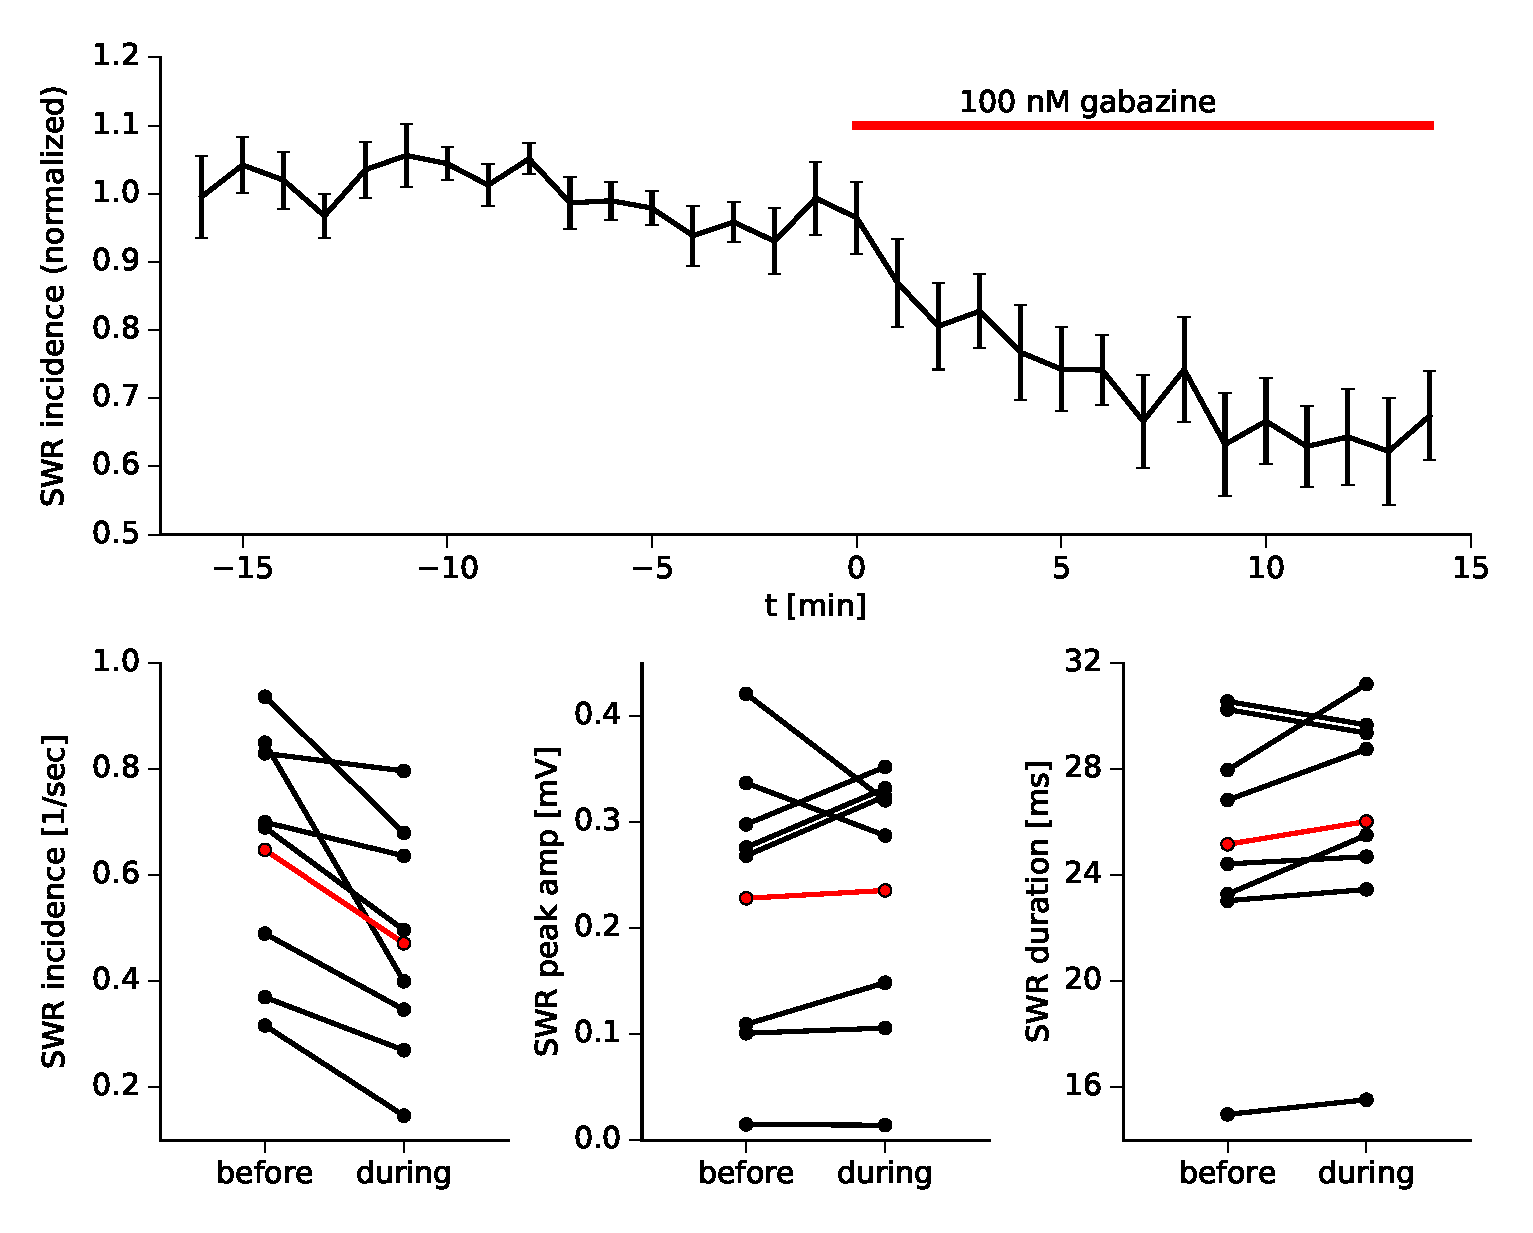
\includegraphics[width =35pc]{gabazine_events_all.eps}
      \caption{
        $\rm GABA_AR$ antagonist gabazine effects on sharp waves. {\bf top}: SW
        incidence in time aggregated from all recordings ($n=8$), where the
        incidence is normalized to 1 by dividing by the mean incidence from before
        the drug application. The red bar shows the time of drug application.
        {\bf bottom:} The average SW incidence, peak and duration measured in
        5-minutes time windows before ([-7, 2] minutes) and during ([6, 11]
        minutes) gabazine application for each slice are denoted with black
        dots. The red dots are the averages from all slices.
      }
      \label{fig:gabazine_sum}
    \end{figure}

    To better characterize how the drug affects the network dynamics, further,
    the analysis focuses on the events in constrained time windows only. Events
    from the window [-7, -2] minutes (before drug application) and [6, 11]
    minutes (after drug application) were used to calculate properties of SWs
    (Figure~\ref{fig:gabazine_sum} bottom row). As already mentioned, there is
    a significant effect on the incidence (around 37\% decrease on average).
    However, somewhat weaker effects are observed on the SW peak amplitude and
    duration.  On average, events tend to get bigger after gabazine
    application. 4 out of 8 recordings show significant (p-value$<0.002$)
    increase in SW amplitude peak after the drug application, and 2/8 show a
    decrease in amplitudes. It is not known whether this increase in amplitudes
    is due to direct effects of gabazine or because of the decreased incidence,
    and thus longer recovery time. 

    The found effect on the SW amplitude is in odds with the finding of
    \citep{Schlingloff2014} who showed that a local puff of gabazine \textit{in
    vitro} decreases the SWR amplitude around the application site
    (Figure~\ref{fig:schlingloff_gabazine}). A possible explanation is that the
    incidence in \citep{Schlingloff2014} is intact as SWRs occur at other
    locations of the slice that are unaffected by the drug. The puffed
    location, however, needs more time to recover from previous events and,
    therefore, the frequent events occurring elsewhere can not engage fully the
    affected subnetwork. In the slices used in our analysis, however, the
    gabazine infusion is global, which results in a slight increase of the SWR
    peaks and also a decrease of the incidence.
    
    \begin{figure}
      \includegraphics[width =35pc]{Schlingloff_3bcd5e.png}
      \caption{A local application of gabazine decreases the amplitude of the
        local SWRs (B) and also decreases the multiunit activity during SW
        events (C, D). Gabazine puffed in the somatic region of PVBCs leads to
        an increased firing and removes the ripple-lock firing of PVBCs. This
        figure is adopted with permission? from \cite{Schlingloff2014}.
      }
    \label{fig:schlingloff_gabazine}
    \end{figure}

    Does gabazine have an effect on the serial correlation between consecutive
    events? To answer this question, the serial correlations (peak-interval and
    interval-peak) were measured before and after drug application in 5-minute
    time windows as described above (Figure~\ref{fig:gabazine_SCsumm}). While
    the peak-interval correlation remains low and does not change after the
    gabazine application, there is a trend of increase in the interval-peak
    correlation. Showing the relation between incidence and interval-peak
    correlation for individual recording (Figure~\ref{fig:gabazine_SCsumm})
    reveals the tendency of decreasing incidence and increased interval-peak
    correlations (6 out of 8 recordings).

    \begin{figure}
      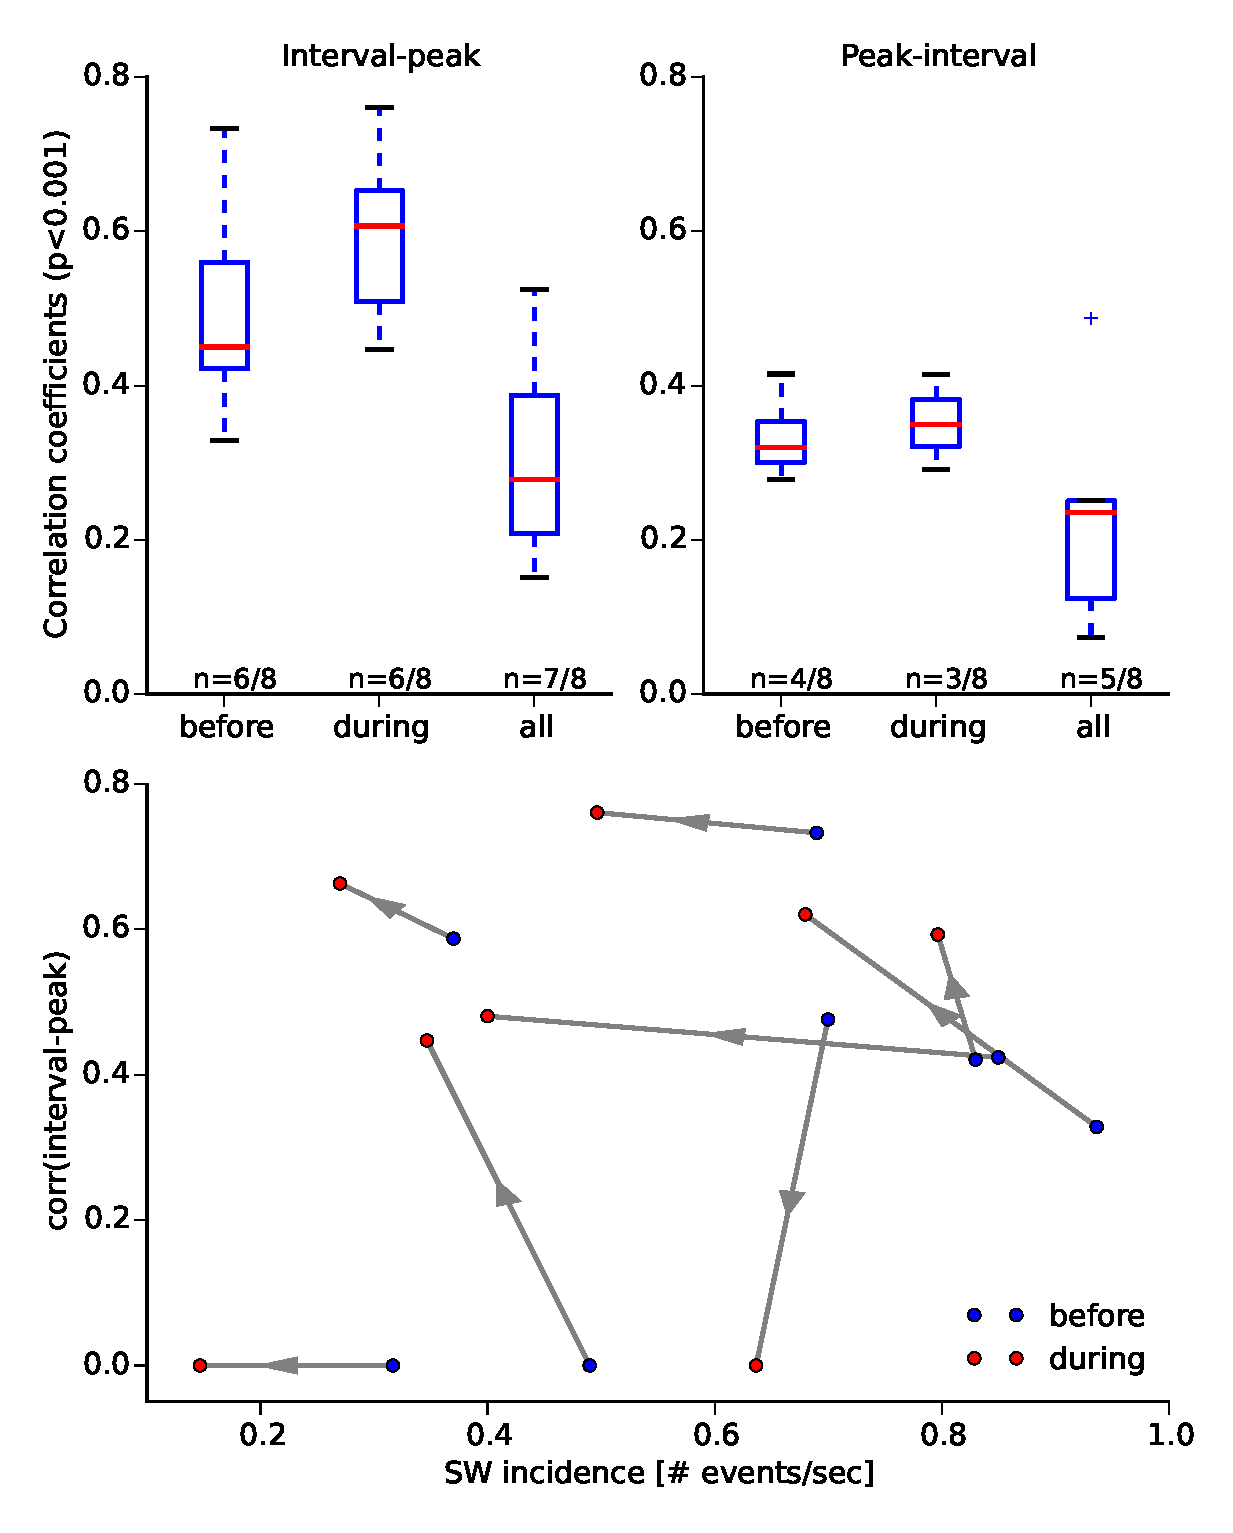
\includegraphics[width= 30pc]{gabazine_SCsumm.eps}
      \caption{
        Gabazine effect on the serial (interval-peak) correlations. \textbf{top:} Serial
        correlation before and during gabazine are calculated in 5-minute long
        time windows, where $n$ shows the number of recordings with significant
        correlations ($p<0.001$) before gabazine application (before), during
        application (during), and aggregated data from the whole recording (all). \textbf{bottom:}
        Serial correlations coefficients between time interval since last event and the following SW
        peak are plotted against recorded incidence; arrows show the change
        after gabazine application.
             }
    \label{fig:gabazine_SCsumm}
    \end{figure}

    In summary, gabazine has the contra-intuitive effect of decreasing the
    incidence of SWRs. Moreover, gabazine application has weak effects in
    increasing the SWR amplitudes and the serial correlations between
    inter-sharp-wave interval and the peak of the following SWR. However, due
    to the small dataset (8 recordings), I can not present a conclusive
    evidence of the drug effects.

  \subsection{Gabazine influence on SWR incidence {\textit {in silico} }}
    \label{sec:gabazine_insilico}
    To better understand how gabazine affects the incidence of SWRs
    {\textit {in silico}}, I deploy the assembly-sequence concept (described in
    Chapter~\ref{chap:memoryreplay}) as a model for the spontaneously occurring
    SWs. Here, numerical simulations of balanced networks with embedded assembly
    sequences and a linear firing rate model are used as tools to describe the
    network dynamics under the influence of gabazine.
      
    In the numerical simulations, sequences of neural assemblies consisting of
    both excitatory and inhibitory neurons are embedded into a randomly
    connected network. Recurrent connectivity ($p_{\rm rc}=0.08$) describes the
    connection probability within an assembly while a feedforward connectivity
    ($p_{\rm ff}=0.06$) is the connectivity between the excitatory neurons of
    consequent assemblies in the sequence (sketch of network connectivity is
    shown in Figure~\ref{fig:net_sketch}). With these parameters values, noise
    fluctuations in the firing rates get amplified by the feedforward structure
    resulting in spontaneous replays (Figure~\ref{fig:spontan}). For a more
    detailed description of the numerical model and the parameter values,
    please refer to Chapter~\ref{chap:memoryreplay}. Here, the effects of
    gabazine are modeled simply by decreasing the conductances of the targeted
    inhibitory synapses with a fixed rate (i.e., $5\%$).

    Not surprisingly, gabazine drastically increased the rate of spontaneous
    replays of assembly sequences in the modelled network. This is illustrated
    in Figure~\ref{fig:gabzine_sim}, where gabazine is applied to all inhibitory
    synapses after the $21^{\rm st}$~second of the simulation. The top two
    panel show raster plots of the excitatory and inhibitory neurons where the
    black dots show individual spikes, and the black stripes are burst of
    synchronous activity during which many neurons fire in close temporal
    proximity. The replays during these activity bursts are used as a model of
    the sharp-wave events. The frequency of these population events is
    increased immediately after the simulated gabazine infusion, as seen in the number of
    replays (the top panel), and in the firing rates (third panel). This result
    is in direct opposition with the gabazine effects that are reported
    {\textit{in vitro}} (Section~\ref{gabazine_invitro}).

    \begin{figure}
      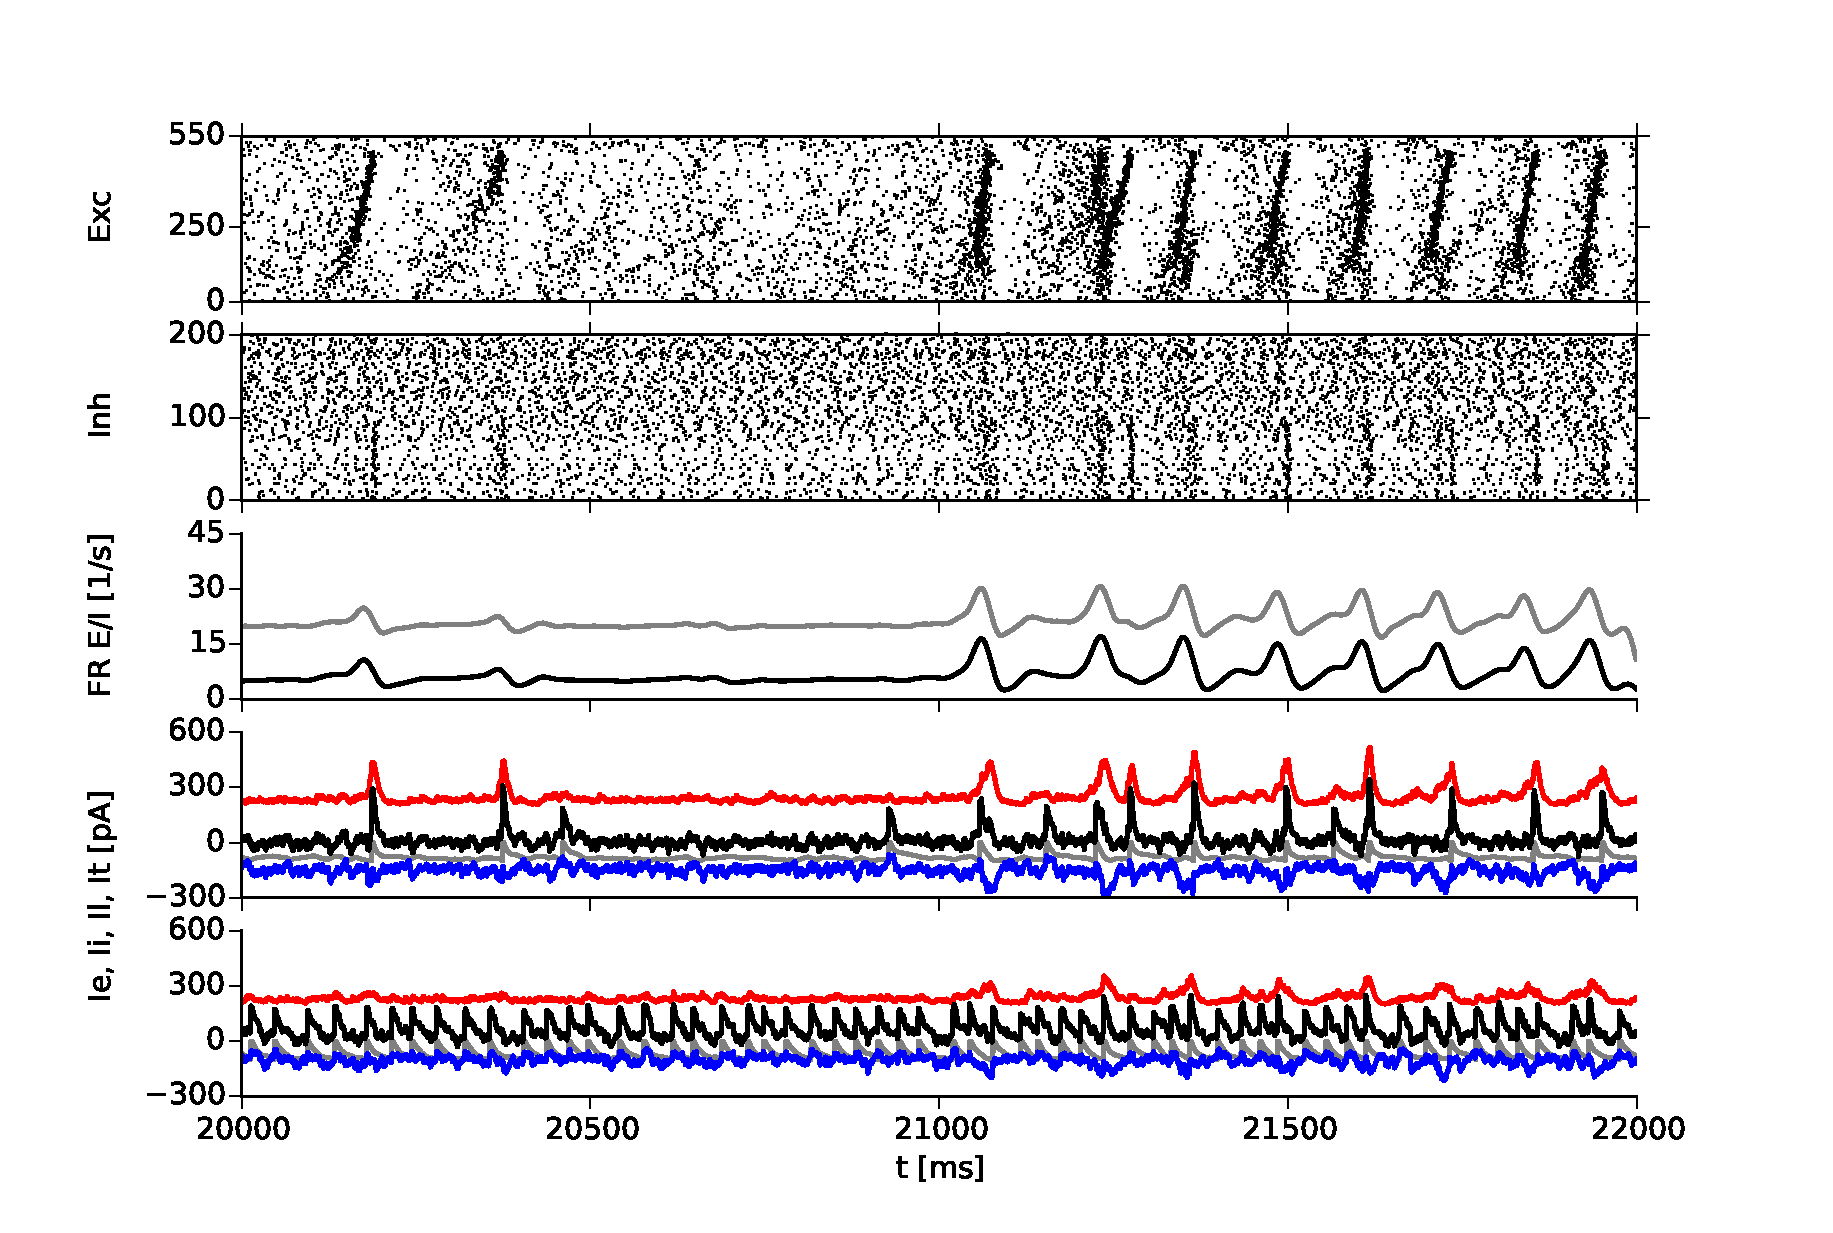
\includegraphics[width =35pc]{gabazine_sim.eps}
      \caption{
        Gabazine {\it in silico} increases the rate of spontaneous replays.
        Decreasing all inhibitory conductances (at $21^{\rm th} \rm second$
        with 5\% leads to increase in the incidence of spontaneous replays in
        balanced-network simulations. The two upper panels show rater plots of
        subpopulations of excitatory and inhibitory neurons, where each black
        dot denotes a spike. Middle plot shows the firing rate of the
        excitatory and inhibitory populations. The last two panels show the
        currents experienced by one excitatory and one inhibitory neuron. Red,
        blue, gray, and black color denote excitatory, inhibitory, leak, and
        total currents.
            }
    \label{fig:gabazine_sim}
    \end{figure}

    Can a relatively simple two-populations balanced network explain the
    gabazine-associated decrease of SWR incidence reported in experiments?
    $\rm GABA_A$ receptors ($\rm GABA_A R$) are known to be complex channels
    with six subunits that can come in various combinations (for the curious
    readers, see Section~\ref{sec:gabaa_intro}). The expressed subunits largely
    determine the receptor properties, i.e., time constants, affinity to GABA
    and other neurotransmitters. For example tonic $\rm GABA_A R$ are
    insensitive for gabazine at low concentrations while phasic $\rm GABA_A R$
    show various affinities depending on the subunit expression. The subunit
    expression is largely determined by the type of the postsynaptic neuron and
    by the location of the channels on the morphological tree
    \ref{???}. One hypothesis to explain the gabazine-associated decrease of SW
    events relies on the assumption that gabazine has differential effects on
    the different $\rm GABA_A$ synapses. And more specifically, if
    inhibitory-to-inhibitory synapses are affected to a larger degree than the
    inhibitory-to-excitatory synapses, one would expect a network that is less
    disinhibited, and thus, the excitatory population receives more inhibition
    resulting in smaller firing rates. In what follows, I test whether such
    assumptions would really decrease the incidence of modeled events.

    As a toy example in numerical simulation, I consider the extreme case where
    gabazine affects the inhibitory-to-inhibitory synapses only. As expected,
    the firing rate of the excitatory neurons is decreased
    (Figure~\ref{fig:gabazine_sim_giionly}). However, the network shows a
    decrease in the firing rate of the inhibitory population as well. How is it
    possible that excitatory neurons receiving weaker inhibition (smaller input
    rate), fire less? To better understand the effects of gabazine, further, I
    present an analytical approach.
    
    \begin{figure}
      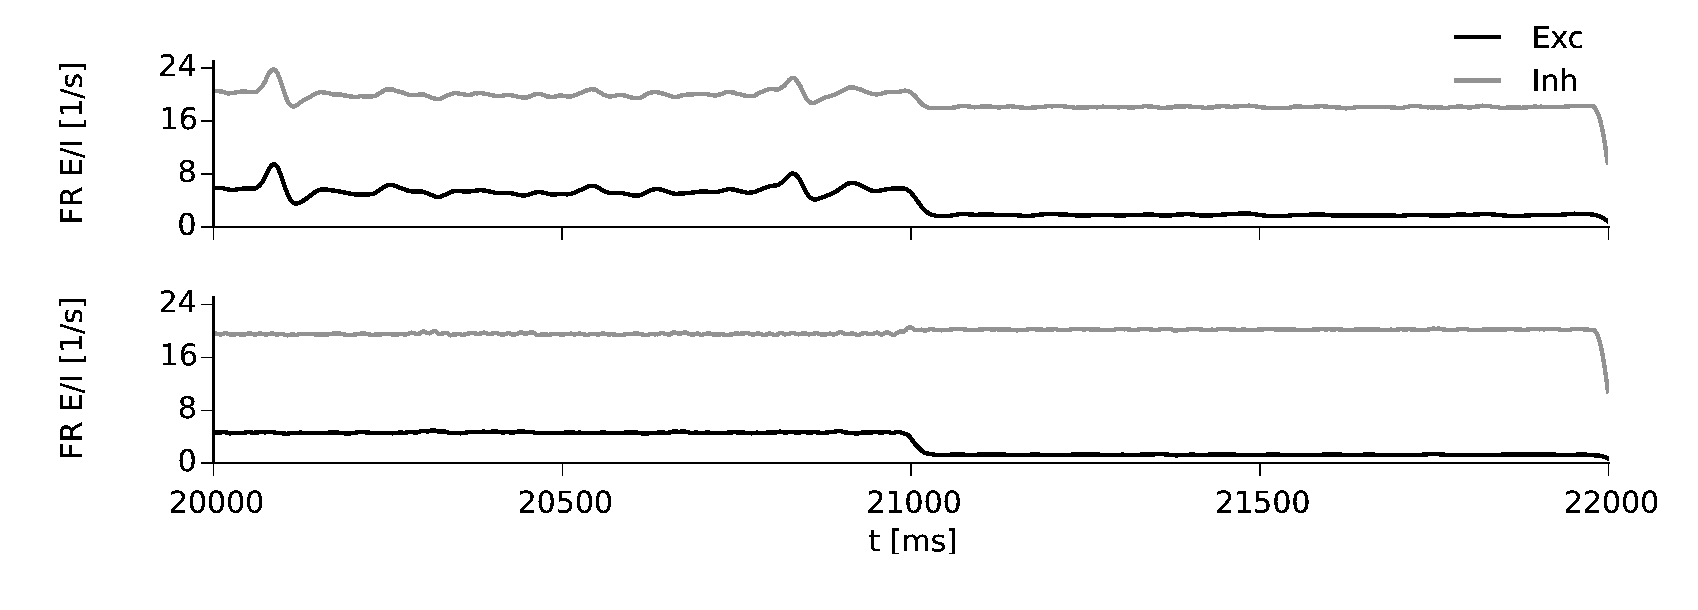
\includegraphics[width =35pc]{gabazine_sim_gii.eps}
      \caption{
        Gabazine {\it in silico} applied only to inhibitory-to-inhibitory synapses
        decreases the rate of spontaneous replays. {\bf top:} Spontaneous replays
        occur during the peaks of the excitatory and inhibitory firing rates. 
        Decreasing the inhibitory-to-inhibitory conductances (at $21^{\rm th} \rm second$
        with 5\% decreases of firing rates and abolishes the spontaneous replays in
        balanced-network simulations. {\bf bottom:} Figure-out what I did! small gee?
      }
    \label{fig:gabazine_sim_giionly}
    \end{figure}

    To capture the network dynamics, I apply a linear model of a two-population
    balanced network and analyse how the rates depend on gabazine. The network
    dynamics is described by the system of differential equations:
    \begin{equation}
      \begin{split}
        \tau \frac{\text{d}r^E}{\text{d}t} &= - r^E + w_{\rm ee} \, r^E -w_{\rm ei} \, r^I + I_0\\
        \tau \frac{\text{d}r^I}{\text{d}t} &= - r^I + w_{\rm ie} \, r^E -w_{\rm ii} \, r^I + I_0\\
      \end{split}
      \label{eq:balanced_net}
    \end{equation}
    where $r^E$ and $r^I$ are excitatory and the inhibitory firing rates,
    respectively. The connection from population $x$ to $y$ is described by the
    connection weight $w_{\rm yx}$ ($x,y = e, i$). The population time constant
    is $\tau$, and the external input to the populations is denoted with $I_0$.

    Assuming that the network is in a steady state, then the rates are
    constant, i.e., $ \frac{\text{d}r^E}{\text{d}t} = 0$ and
    $\frac{\text{d}r^I}{\text{d}t} = 0 $. In this condition, one can express
    the stationary solution:
    \begin{equation}
      \begin{split}
        r^E &= \frac{(1+w_{\rm ii} - w_{\rm ei})}{w_{\rm ie}w_{\rm ei} -
                (1+w_{\rm ii})(-1+w_{\rm ee})} I_0 \\
        r^I &= \frac{(1+w_{\rm ie} - w_{\rm ee})}{w_{\rm ie}w_{\rm ei} -
                (1+w_{\rm ii})(-1+w_{\rm ee})} I_0
      \end{split}
      \label{eq:balanced_sol}
    \end{equation}
  
    To estimate how gabazine-induced decrease of inhibitory connections
    affects the firing rates, we can look at the derivatives of the
    steady-state rates in respect to the gabazine concentration $c_{\rm gbz}$:
    \begin{equation}
      \frac{\partial r^E}{\partial c_{\rm gbz}} =
      \frac{\partial r^E}{\partial w_{\rm ei}} \cdot \frac{\partial w_{\rm ei}}{\partial c_{\rm gbz}} + 
      \frac{\partial r^E}{\partial w_{\rm ii}} \cdot \frac{\partial w_{\rm ii}}{\partial c_{\rm gbz}}
      \label{eq:re_chain}
    \end{equation}
    and
    \begin{equation}
      \frac{\partial r^I}{\partial c_{\rm gbz}} =
      \frac{\partial r^I}{\partial w_{\rm ei}} \cdot \frac{\partial w_{\rm ei}}{\partial c_{\rm gbz}} + 
      \frac{\partial r^I}{\partial w_{\rm ii}} \cdot \frac{\partial w_{\rm ii}}{\partial c_{\rm gbz}}.
      \label{eq:ri_chain}
    \end{equation}

    The partial derivatives of inhibitory weights ($w_{\rm ei}$ and $w_{\rm
    ii}$) in respect to the drug concentration $c_{\rm gbz}$ is negative due to
    the antagonist  effects of gabazine. The partial derivatives of the rates
    in respect to the inhibitory weights can easily be estimated from
    Equation~\ref{eq:balanced_sol}:
    \begin{equation}
      \begin{split}
        \frac{\partial r^E}{\partial w_{\rm ii}} &= 
              I_0 \frac{w_{\rm ei} (1 + w_{\rm ie} - w_{\rm ee})} {D^2} \\
        \frac{\partial r^I}{\partial w_{\rm ii}} &=
              I_0 \frac{(-1 + w_{\rm ee})(1 + w_{\rm ie} - w_{\rm ee})} {D^2} \\
      \end{split}
      \label{eq:drdwii}
    \end{equation}

    \begin{equation}
      \begin{split}
        \frac{\partial r^E}{\partial w_{\rm ei}} &=
              I_0 \frac{-(1 + w_{\rm ii}) (1 + w_{\rm ie} - w_{\rm ee})} {D^2} \\
        \frac{\partial r^I}{\partial w_{\rm ei}} &=
              I_0 \frac{-w_{\rm ie} (1 + w_{\rm ie} - w_{\rm ee})} {D^2} \\
      \end{split}
      \label{eq:drdwei}
    \end{equation}
    where $D=w_{\rm ie}w_{\rm ei} - (1+w_{\rm ii})(-1+w_{\rm ee})$.
    
    If we now assume that gabazine has the same effect on all inhibitory
    synapses, i.e., $\frac{\partial w_{\rm ei}}{\partial c_{\rm gbz}} =
    \frac{\partial w_{\rm ii}}{\partial c_{\rm gbz}}$, the change of firing
    rate due to gabazine is:
    \begin{equation}
      \begin{split}
        \frac{\partial r^E}{\partial c_{\rm gbz}} &=
            \frac{\partial w_{\rm ii}}{\partial c_{\rm gbz}} \cdot
            I_0 \frac{-(1 + w_{\rm ii} - w_{\rm ei}) (1 + w_{\rm ie} - w_{\rm ee})} {D^2} =
            - \frac{\partial w_{\rm ii}}{\partial c_{\rm gbz}} \cdot \frac{r^E r^I}{I_0} > 0 \\
        \frac{\partial r^I}{\partial c_{\rm gbz}} &=
            \frac{\partial w_{\rm ii}}{\partial c_{\rm gbz}} \cdot
            I_0 \frac{- (1 + w_{\rm ie} - w_{\rm ee})^2} {D^2} =
            - \frac{\partial w_{\rm ii}}{\partial c_{\rm gbz}} \cdot \frac{r^I r^I}{I_0} > 0 \\
      \end{split}
      %\label{eq:x}
    \end{equation}
    In line with the simulations, the derivatives above are always positive (if
    $\frac{\partial w_{\rm ii}}{\partial c_{\rm gbz}} < 0 $), i.e., gabazine
    always increases the rate of both excitatory and inhibitory
    populations. 

    Can this linear model model explain the simulation results in which
    gabazine affects only inhibitory-to-inhibitory synapses? There we saw a
    decrease not only in the excitatory but also in the inhibitory firing rates
    (Figure~\ref{fig???,bottom?}). Taking the rate derivatives in respect to
    $w_{\rm ii}$ only (In Equations~\ref{eq:re_chain} and \ref{eq:ri_chain}, we
    assume that $\frac{\partial w_{\rm ei}}{\partial c_{\rm gbz}} = 0$):

    \begin{equation}
      \begin{split}
        \frac{\partial r^E}{\partial c_{\rm gbz}} &=
            \frac{\partial w_{\rm ii}}{\partial c_{\rm gbz}} \cdot
            I_0 \frac{w_{\rm ei}(1 + w_{\rm ie} - w_{\rm ee})} {D^2} =
            \frac{\partial w_{\rm ii}}{\partial c_{\rm gbz}} \cdot \frac{w_{\rm ei}}{D} \cdot r^I \\
        \frac{\partial r^I}{\partial c_{\rm gbz}} &=
            \frac{\partial w_{\rm ii}}{\partial c_{\rm gbz}} \cdot
            I_0 \frac{(-1+w_{\rm ee}) (1 + w_{\rm ie} - w_{\rm ee})} {D^2} =
            \frac{\partial w_{\rm ii}}{\partial c_{\rm gbz}} \cdot \frac{-1+w_{\rm ee}}{D} \cdot r^I \,\, . \\
      \end{split}
      %\label{eq:x}
    \end{equation}
 
    Here, the sign of the determinant $D$ from Equation~\ref{eq:balanced_net}
    determines the change in firing rate. Let us first assume that $D<0$. To
    fulfil the requirement for positive firing rates (i.e., $r^I>0$ in
    Equation~\ref{eq:balanced_sol}), then $w_{\rm ee}>1+w_{\rm ie}$ should be
    fulfilled. However, this is unlikely to be the case as the excitatory
    conductances used in the simulations are all equal $g_{\rm ee}=g_{\rm ie}$.
    Therefore, I conclude that $D>0$. In that case, it is easy to see that
    $\frac{\partial r^E}{\partial c_{\rm gbz}} < 0$, meaning that excitatory
    rate decreases when $w_{\rm ii}$ is depressed. This line of arguments is
    supported by the simulations, where gabazine applied to the
    inhibitory-to-inhibitory connections only decreases the excitatory firing
    rate (Figure~\ref{fig:gabazine_sim_giionly}). On the other hand, $r^I$
    shows more interesting behaviour that depends on the excitatory weights.
    For intermediate values $w_{\rm ee} \in (1, 1+w_{\rm ie})$, the inhibitory
    rate decreases during gabazine application as well (as seen in
    Figure~\ref{fig:gabazine_sim_giionly}, top panel). For values of $w_{\rm
    ee}$ outside of this interval, one would expect increase of inhibitory
    firing after the drug infusion. For the prove of concept, I tested a
    network where $g_{\rm ee}=2 g_{\rm ie}$ and show that in such case the
    inhibitory rate goes up after the simulated drug application
    (Figure~\ref{fig:gabazine_sim_giionly}, bottom panel).
    %To test again whether low/high wee increases ri!!!!
    %I tested that by using lower (5 times smaller than default)
    %and higher (5 times larger than default) excitatory-to-excitatory
    %connectivity in the numerical model and found that inhibitory rate is
    %indeed increased (not shown here).

    To summarize the results from this section, by using numerical simulations
    and a linear analytical description, I showed that in a balanced network a
    gabazine application is increasing the firing rates of both inhibitory and
    excitatory populations. This increase of firing leads to higher incidence
    of spontaneous replays which is in odds with the counterintuitive decrease
    of incidence observed {\textit {in vitro}}. Therefore, I tested whether a
    differential effect of gabazine on different synapses can explain the
    experimental results. I considered the extreme case when gabazine affects
    only inhibitory-to-inhibitory synapses and showed that in this case we can
    always expect decrease in the rate of excitatory population. This result
    suggests that possibly stronger effects of gabazine on the inhibitory
    neurons might explain the decreased SWR incidence after gabazine
    application {\textit {in vitro}}.
    
    Here I examine a minimal model consisting of only two populations, but
    nevertheless the approach can provide some means for studying {\it in-vitro}
    models. A similar approach can also be applied to the more accurate
    3-population nonlinear model currently developed by Roberta Evangelista,
    and utilized to examine in what conditions gabazine decreases the network
    excitability. Is it possible that in the 3-population model, a gabazine
    application to all inhibitory synapses can decrease the rate of spontaneous
    events? Or would it be required that the disinhibitory synapses (from PVBC
    to the mysterious inhibitory neurons) are affected to a larger degree?

    A strong assumption in the foundation of the current framework is that the
    decrease of SWR incidence is due to decrease of firing of the excitatory
    population. Whether this is indeed the case has to be confirmed from
    {\it in-vitro} experiments. It is also not known how does gabazine affects the
    firing of the inhibitory populations. The simulations show that gabazine
    applied only on the inhibitory-to-inhibitory connections can decrease not
    only the excitatory but also the inhibitory firing rates. This result is
    interesting by its own as the decrease of $r^E$ is counterintuitive. How
    does it come that the excitatory population decreases its firing rate after
    receiving less inhibition due to the decrease of $r^I$? (should I dive into that??)

  \subsection{Involvement of $\rm GABA_B$ receptors in sharp waves}

    Sharp waves are huge population events where many pyramidal cells and
    interneurons are firing with increased firing rates, which is especially
    pronounced for the perisomatic targeting parvalbumin-positive basket cells
    (PVBCs) and the bistratified cells \citep{Klausberger2009}. It has been
    shown that the repetitive firing of interneurons can activate extrasynaptic
    $\rm GABA_B$ receptors possibly through increased concentrations of ambient
    GABA in the extracellular space \cite{Wang2010,??}. The inhibition from
    $\rm GABA_B Rs$ is relatively slow, lasting several hundreds of
    milliseconds, which is close to the time scale of the typical inter-SW
    intervals. Here, I study the possibility that the relatively long time
    intervals between SW events are determined by $\rm GABA_B Rs$.
    
    First, to investigate whether $\rm GABA_B$ is involved in the SW incidence
    in the {\textit{in-vitro}} model, I analysed extracellular recordings where
    the $\rm GABA_B R$ antagonist SCH50,911 (further referred as SCH) was
    applied in slices. The number of analysed slices is 12 (see the Methods
    section). An example of the SCH effects in a slice are shown in
    Figure~\ref{fig:gB_example}. The drug effects are reflected in the network
    dynamics already during the first minute of application by increasing the
    incidence of SWs (Figure~\ref{fig:gB_example}, top panel). An independent
    two-sample t-test of the incidence (measured as number of events per sweep
    in confined 5-minute time intervals) show a significant increase of
    incidence (p-value $<10^{-7}$). Other main properties, such as, peak
    amplitude and duration are decreased after the SCH application (p-values
    $<10^{-10}$, and $<10^{-3}$, respectively).
    
    \begin{figure}
      %\includegraphics[width =35pc]{19march13_slice1.png}
      \includegraphics[width =35pc]{20jan12_slice2.png}
      \caption{ 
        Extracellular recording from the CA3 area where SCH50,911 is applied to
        the hippocampal slice. The time of drug application is denoted with a
        horizontal red bar. The top panel shows the SW incidence in time with a
        minute time resolution. The two panels below show the SW amplitude
        peaks, where `fil' and `raw' stand for band-passed filtered ($\sim
        5-50\, \rm Hz$, for details see the Methods section) and raw voltage
        traces, respectively; units are in mV. The gray dots represent single
        events, and the black lines represent the mean and the standard
        deviation of the amplitude peak in a minute time window. Analogously,
        the forth panel shows the SW duration in milliseconds. The panels on
        the bottom row show all events before (left) and during (middle) drug
        application overlaid in gray, and the mean wave-forms are in black. The
        right-most panel shows a comparison between the mean events from before
        and during SCH application.
              }
    \label{fig:gB_example}
    \end{figure}

    Blocking the $\rm GABA_B Rs$ resulted in increase of the average incidence
    of spontaneous sharp waves from all slices.  The drug effects are visible
    already in the first minute after the application and saturate around 2-3
    minutes later (Figure~\ref{gB_summ}, top panel). To better assess the
    effects of SCH further, the analysis focuses on the events in 5-minutes
    long time windows, i.e., in the intervals [-5, 0] that is before and [2, 7]
    minutes that is during drug application. Comparing the data from these two
    intervals shows that SCH increases the incidence in every recording, and
    10/12 show a significant increase (independent 2-sample t-test;
    p-value$<0.002$). On average, SCH resulted in decrease of SW amplitudes
    (Figure~\ref{gB_summ}, bottom middle panel), where 6/12 slices show
    a significant decrease (p-value$<0.001$), and in 2/12 slices the amplitudes
    were increased (p-value$0.001$). The duration of sharp waves, also
    decreases on average, but however, this change is not significant
    (p-value$>0.01$ in 11/12 slices). While the result for every recording
    varies depending on the exact 5-minute time windows that are used for the
    analysis, the summary results do not change qualitatively.
    
    \begin{figure}
      \includegraphics[width =35pc]{SCH_all.eps}
      \caption{
        $\rm GABA_BR$ antagonist SCH50,911 effects on sharp waves. {\bf top}:
        SW incidence in time aggregated from all recordings ($n=12$), where the
        incidence is normalized to 1 by dividing by the mean incidence before
        the drug application. The red bar shows the time of drug application.
        {\bf bottom:} The average SW incidence, peak and duration measured in
        5-minutes time windows before ([-5, 0] minutes) and during ([2, 7]
        minutes) SCH application for each slice are denoted with black dots.
        The red dots are the averages from all slices.
            }
    \label{gB_summ}
    \end{figure}

    Next, I inquire whether blocking $\rm GABA_B Rs$ affects also the serial
    correlation between events. At first glance the pooled data does not reveal
    any change in the correlations, as the correlation distributions from
    before and during SCH application (Figure~\ref{gB_SCsumm}, top panels) are
    statistically similar. However, looking at the effects in the individual
    recordings (Figure~\ref{gB_SCsumm}, bottom panel) one can see that there is
    a decrease of serial correlation after drug application in 10 out of 12
    slices (the 2 remaining recordings show no significant correlations).

    \begin{figure}
      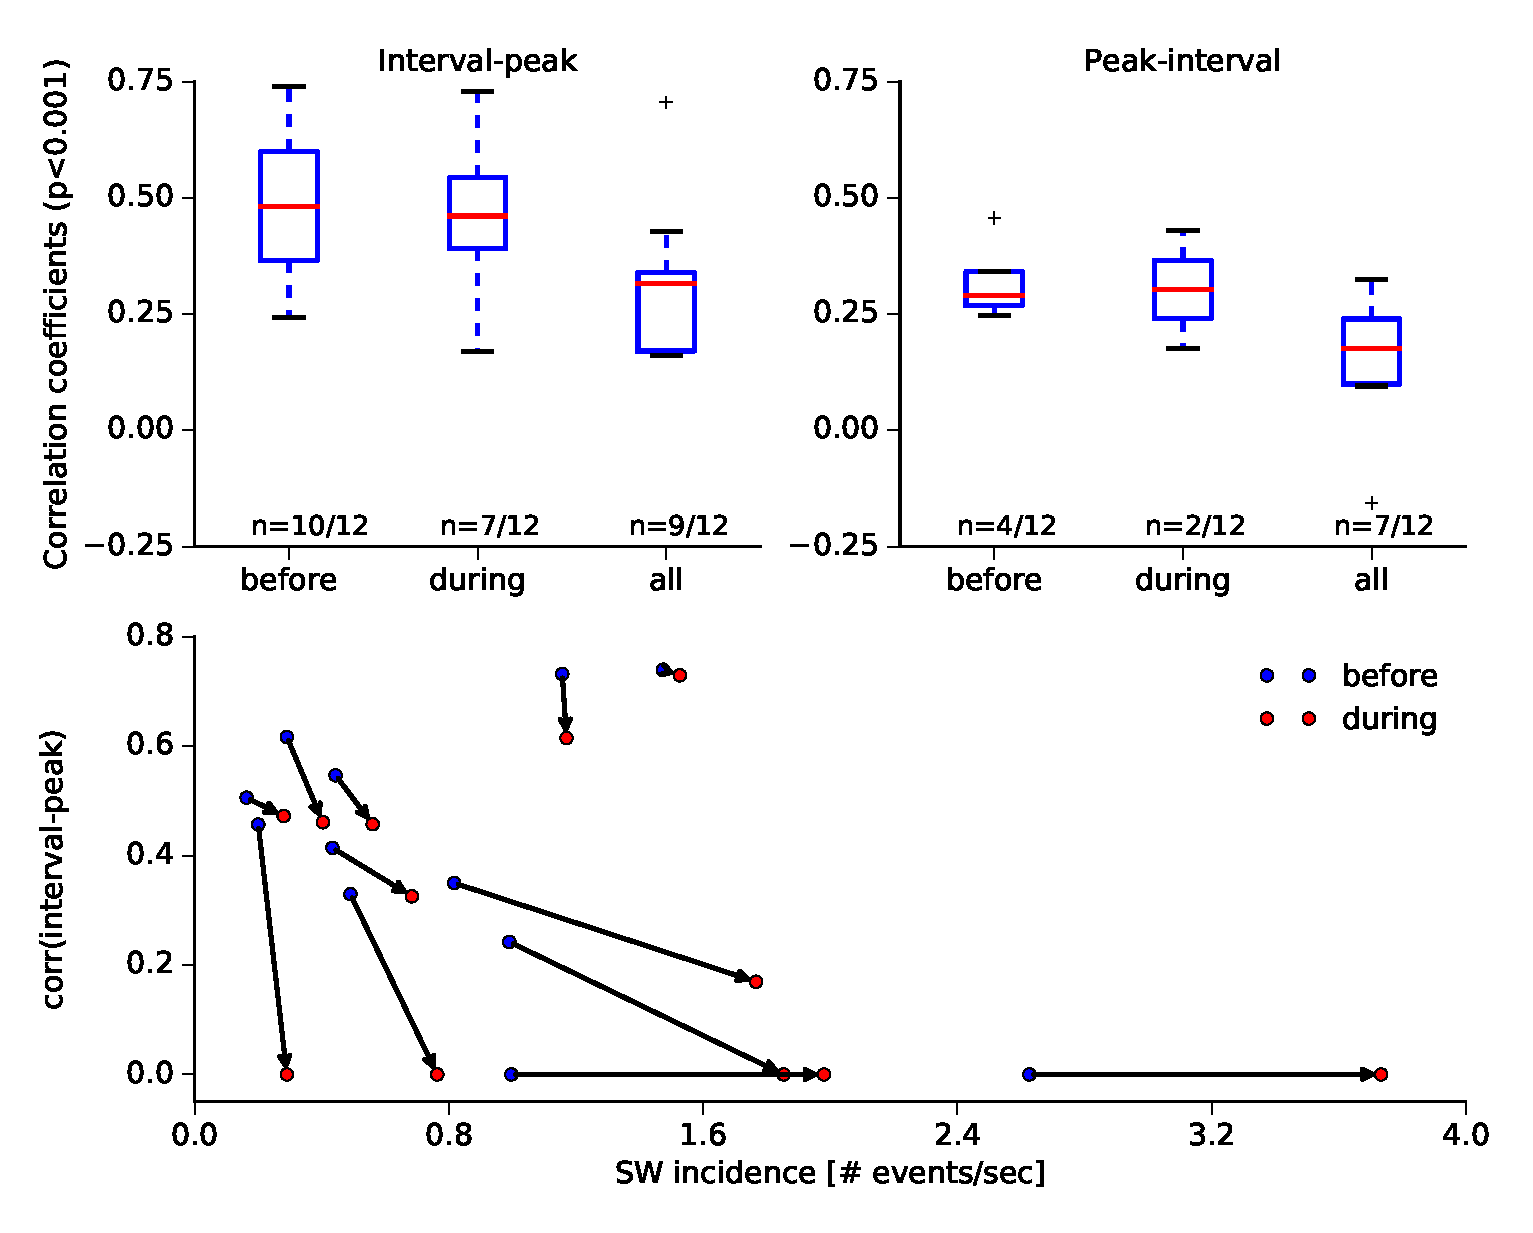
\includegraphics[width =35pc]{SCH_SCsumm.eps}
      \caption{
        $\rm GABA_BR$ antagonist SCH50,911 effect on the serial (interval-peak)
        correlations. \textbf{top:} Serial correlation before and during
        gabazine are calculated in 5-minute long time windows, where $n$ shows
        the number of recordings with significant correlations ($p<0.001$)
        before SCH application (before), during application (during), and
        aggregated data from the whole recording (all). \textbf{bottom:} Serial
        correlations coefficients between time interval since last event and
        the following SW peak are plotted against recorded incidence; arrows
        show the change after SCH application.
            }
    \label{gB_SCsumm}
    \end{figure}

    To summarize the findings above, $\rm GABA_B Rs$ are taking part in the SW
    modulation by increasing the incidence and decreasing the peaks of SWs.
    However, the increase in incidence is on average less than two-fold
    suggesting that there are other mechanisms different than $\rm GABA_B$ that
    act on a slow time scales and are involved in controlling the incidence.
    Moreover, blocking $\rm GABA_B Rs$ leads to a decrease in the serial
    correlations between interval and peaks, which is puzzling given the
    increased incidence. Intuitively, one could expect that the serial
    correlations are stronger for higher incidences, and weaker for lower
    incidences when the system depletion is recovered. To investigate how does
    $\rm GABA_B Rs$ influence the SW incidence, it is worth having a closer
    look at the possible involvement of the different $\rm GABA_B$ channels.

    It is been shown that a repetitive firing of certain interneurons can evoke
    slow and strong inhibition due to activation of postsynaptic or
    extrasynaptic $\rm GABA_B$ receptors on pyramids \citep{Scanziani2000,
    Gassmann2012}. As sharp waves are population events that recruit many
    neurons, and especially the perisomatic targeting interneurons
    \citep{Klausberg2009} it is likely that ambient GABA in this region is
    increased \citep{Hollnagel2014, Lang2014}. Next, I ask whether $\rm
    GABA_BRs$ located postsynaptically on pyramidal cells are indeed activated
    after SWs, and whether they play any role in the modulation of SWs. To test
    this hypothesis, here I analyse data from simultaneous (paired)
    extracellular and intracellular recordings performed in the radiatum layer
    of the hippocampal CA3 area and a pyramidal cell in the CA3, respectively.
    By averaging the intracellular traces across events, we can see that a GB
    hyperpolarization is present in a few recordings, but is not is not visible
    in the mean of all recordings (Figure~\ref{fig:intra_means}, top panel).
    Most intracellular traces show various combination of depolarization and
    hyperpolarization, indicating a rich dynamics of excitatory and inhibitory
    inputs. In the recordings that show a slow hyperpolarization (4 out of 13
    recordings, shown in Figure~\ref{fig:intra_means}, bottom panel) the trough
    in the membrane potential is around $200 \, \rm ms$ after the population
    event and lasts for about $500 \, \rm ms$. Interestingly, only one
    recording reveals well-pronounced slow as well as fast inhibition (red
    trace).

   \begin{figure}
      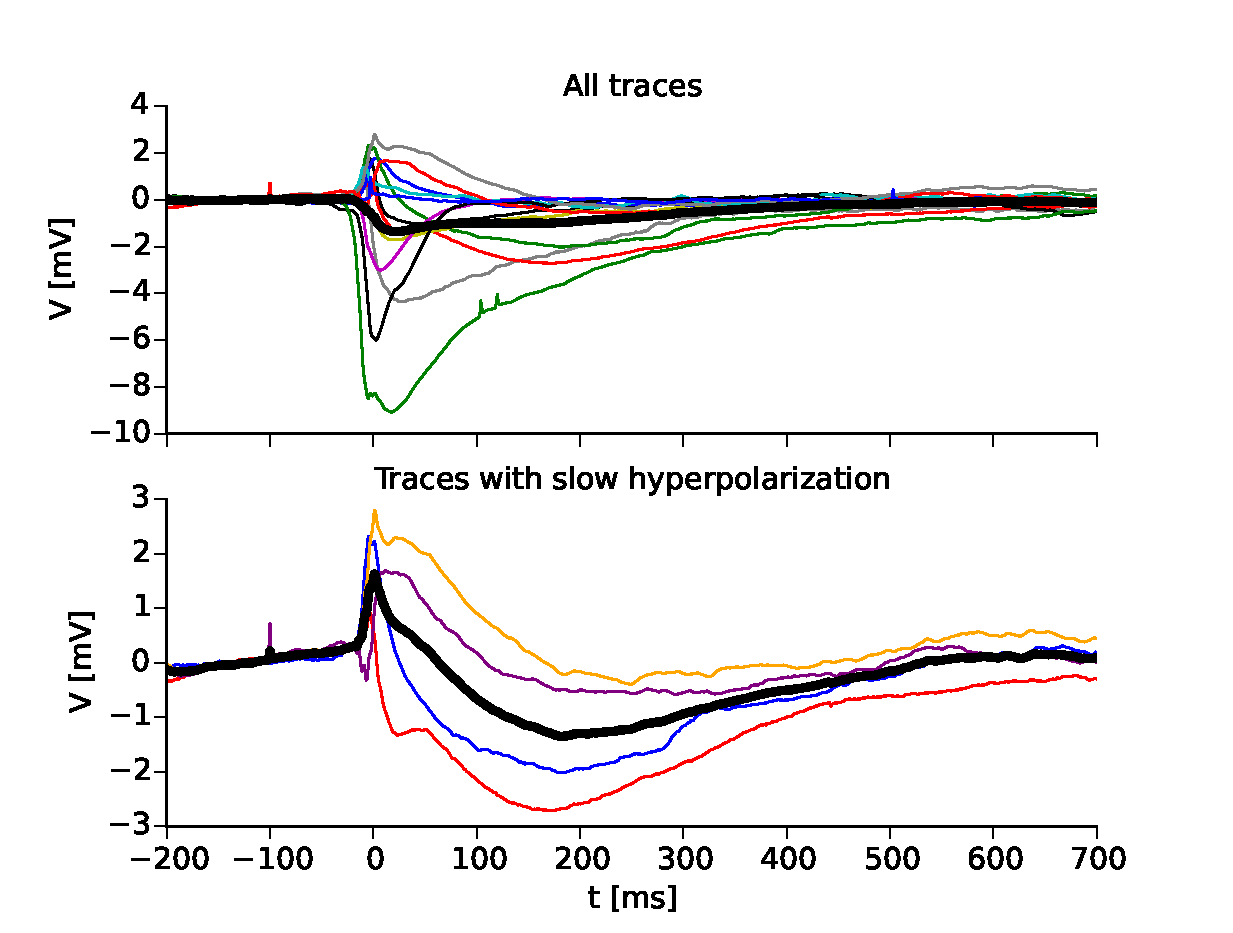
\includegraphics[width =30pc]{mean_intras.eps}
      \caption{ 
        Simultaneous extracellular and intracellular recordings in slices. {\bf
        top:} Intracellular recordings from patched pyramidal cells during
        sharp waves. The mean voltage traces associated to SWs from each slice
        are color coded; the thick black line is the mean of the means. {\bf
        bottom:} Mean voltage traces of cells that show slow, possibly $\rm
        GABA_BR$-evoked hyperpolarization. All traces are normalized by
        subtracting the mean potential the before the event.
              }
      \label{fig:intra_means}
    \end{figure}

    Is the slow hyperpolarization correlated in any way with the amplitude of
    the SWs? To test this, I separated the events in each recording in two
    groups: big and small events, i.e., the 30\% biggest or 30\%
    smallest events, respectively. Plotting the mean intracellular trace during
    small and big events, shows that the SWs with larger amplitudes are
    associated with larger hyperpolarization (Figure~\ref{fig:intra_big_small},
    top panel). Interestingly, the mean traces before big and small events are
    virtually indistinguishable (Figure~\ref{fig:intra_big_small}, bottom
    panel), suggesting that the hyperpolarization does not determine the size
    of the following event. This result holds for all the four recordings that
    exhibit slow inhibition in the voltage potential.
    
    \begin{figure}
      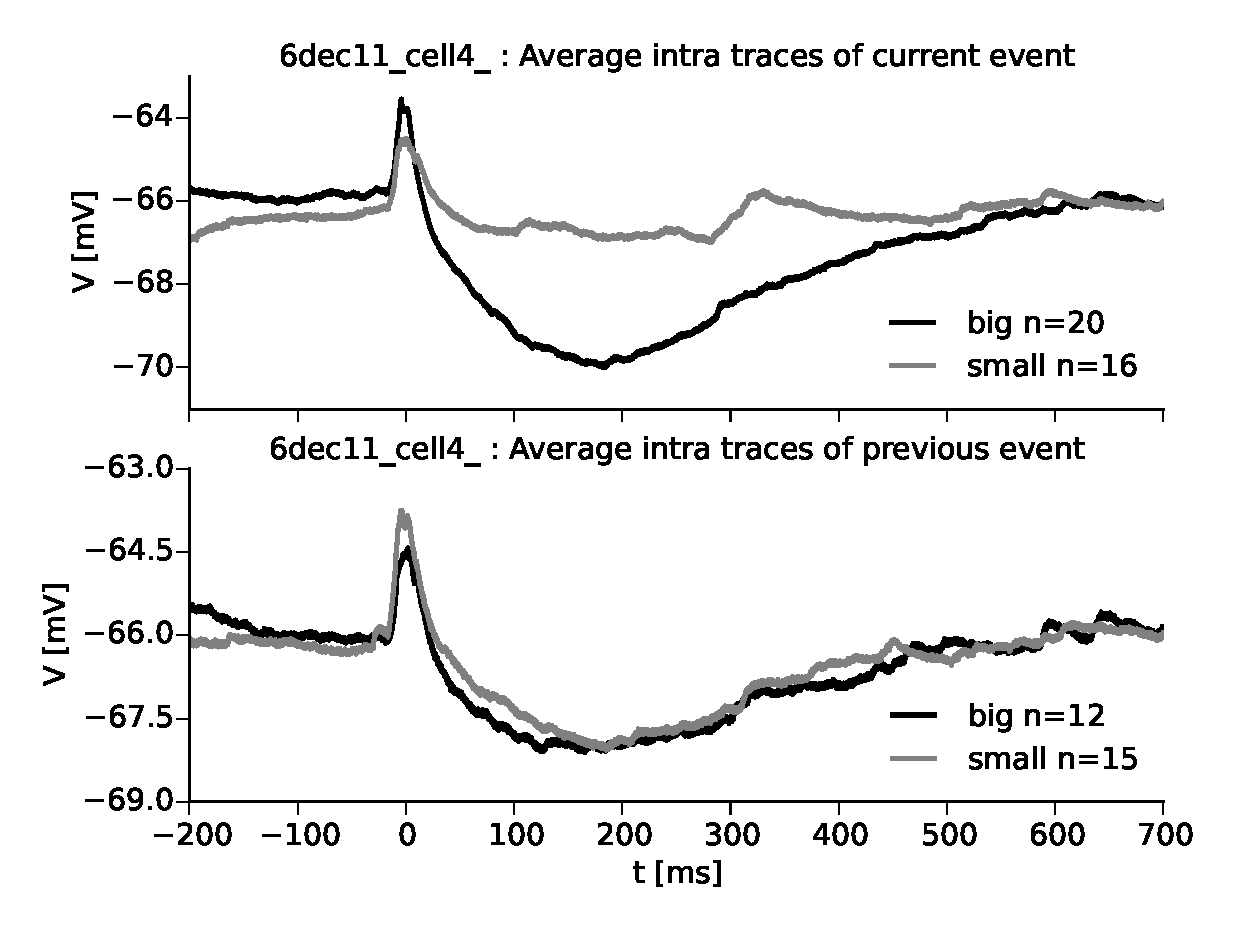
\includegraphics[width =30pc]{6dec11_cell4_000.eps}
      \caption{ 
        Sharp waves with larger peak amplitudes evoke stronger
        hyperpolarization. {\bf top:} Big events (30 \% of the largest SW
        events) are associated with a well-pronounced slow hyperpolarization.
        Smaller events (30\% of the smallest SWs) did not evoke a $\rm
        GABA_B$-associated response. The voltage difference preceding the
        events is a recording artifact (see the Methods section). {\bf bottom:}
        There is no correlation between the depolarisation of a cell and the
        peak amplitude of the following SW event.
              }
    \end{figure}

    Moreover, the slow hyperpolarization does not affect the time interval
    until the following event (not shown here). There is a correlation between
    the interval and the size of the following hyperpolarization, which is
    expected given the fact that longer intervals are followed by larger SWs,
    and thus, larger hyperpolarization.

    The last dataset of intracellular and extracellular recordings reveals that
    slow, possibly $\rm GABA_B$-associated hyperpolarization occurs only in a
    fraction of the CA3 pyramidal neurons {\textit{in vitro}}. The magnitude of
    the received inhibition is not correlated with the size or the time
    interval until the next event. Therefore, I conclude that postsynaptic $\rm
    GABA_B$ receptors do not play a central, if any, role in controlling the
    incidence of sharp-wave ripples.
 
    However, seems not to be crucial for SWRs, but only facilitates a bit?

    In summary, the gB antagonist SCH lead to increase in SW incidence in the in SW vitro model analysed here....?

    presynaptic effects of gB; likely not due to postsynaptic gBR on PY neurons (from simultaneous intra/extra recordings dataset); Maier2012? also suggests presynaptic effects of gB; however
      
    SCH decreases peak
      
    decreased peak means decreased currents; however, blocking presynaptic gBR would lead to increased single IPSC/P; therefore likely that SCH decreases FR of perisomatic targeting INs during SW events

\section{Discussion}

  summary:
    - low peak-interval correlation in comparison to interval-peak
    - SW amplitude is not a local phenomenon

  The exact effects of gabazine on the network activity invitro are not clear.
  It is still an open question how does gabazine change the activity of the PC and the different
  types of INs. 

  Stiedl2006: low concentration of gabazine (500 nM) in hippocmapal slices: only slight increase LFP in striatum rasiatum near pyramidal cell layer

  Schligloff2014 used local puffs of gabazine and showed that MUI activity during SWs in the stratum pyramidale is decreased. However does it also decrease outside of the events? A few more issues with this experiments is.. it was a local puff, and the identity of neurons is not known.

  Experiment suggestions: -

    - quantify network effects of gabazine:
      - measure and compare PC firing before and during gabazine administration
      - same for PVBC and the mysterious INs
    - identify the INs that inhibit PC firing between events.

    Behrens2007: gabazine hyperpolarized cells (in slices which were already induced), 
maybe because of ambient gaba??
  \subsection{Hypothesis on how gabazine affects SWR incidence} 

    %Local gabazine puff decreases the SW peaks in Schilinglof, but is also
    %decreases the MU firing \ref{fig:schlingloff_gabazine}. Cells are more
    %inhibited? However in another experiment the same authors measured PVBCs in
    %a loose patch and show that their FR is increased. This suggests some
  
    Why would gabazine increase the correlations??? especially for decreased
    incidence one would expect decreased correlations because of the longer
    time for synaptic recovery from STD...  The increase of SWR amplitudes
    measured in st. pyr. suggest larger synaptic currents in that region. On
    the other hand, gabazine decreases the synaptic currents from single
    presynaptic release. A plausible conclusion that can be made is that the
    smaller IPSC are compensated by larger firing of the PVBC. The larger PVBC
    firing leads to a stronger the synaptic depression and thus to a longer
    time of synaptic recovery. 

    --- make up a figure sketch of the idea: STP, PVBC FR --- here or in the discussion

   %disinhibitory mechanisms.... pc/PVBC ratio is 95/5 or 98/2...
    
    In summary, PC seems to be less excitable (due to lower FRs), while PVBCs
    fire more when gabazine is applied. Paradox: how does it happen that
    decreasing inhibition decreases SWR incidence, i.e., the network gets less
    excitable or more inhibited? Possible GBr receptor activation???? higher IN
    activity, leads to more gaba, more extrasynaptic activations...then 

  \subsection{Hypothesis on how GABA affects on SWR incidence} 


\section{Methods}
%________________
  The results in this chapter are bases on the analysis of data kindly provided
  by Nikolaus Maier from Schmitzlab. Here, I analyse 5 datasets of {\it in
  vitro} recordings. All the recordings were performed in the CA3 area of
  hippocampal slices. Here I give a brief summary about the datasets and
  provide some details on the techniques applied during the analysis.

  \subsection{Data}
  %________________
    \subsubsection{Dataset 1: gabazine}
     
      8? recordings.
      extracellular field potential, a few tens of minutes after the beginning of recording gabazine is infused in the extracellular solution.
      Sampling rates are between 5 and 10 kHz.
      Multiple sweeps of 30/60 seconds.
      In two recordings there was washout of the gabazine.
      gabazine 


      for further analysis time windows were chosen for the comparisons:
        -12 , -3 before and 6, 11 after the drug infusion.
        time to go home!




    \subsubsection{Dataset 2: SCH50,911}
      The second dataset contains extracellular recordings from 13 slices.
      Here, extracellular field potential is measured for several minutes
      depending on the recording, and later on the drug SCH50,911 was infused
      into the ?solution.  SCH50,911 is a ${\rm GABA_B}$ receptor antagonist
      which acts on presynaptic as well as on postsynaptic receptors.

    , but here I excluded one recording as it exhibits virtually
    no events prior to the drug application, and thus, heavily skews the average
    results.

    \subsubsection{Dataset 3: Extra and Intra}
      The third dataset consists of 13 pairs of recordings.  Each pair contains
      simultaneous extracellular field recording and intracellular recording
      from a patched pyramidal cell in a current clamp mode.  The recordings
      consist of multiple sweeps of around 5-20 seconds.  The length of each
      recording is rather short, ranging from 40 seconds up to 10 minutes.  The
      sampling rates are between 5 and 40 kHz.

  \subsection{Data analysis}
  %_________________________
      To compare the SW sizes, I took the raw peaks of
      the events and normalize them such that for each electrode the mean peak
      is 0, and the std is 1.  becaure of diff location of th electrode..?
      
      independent 2-sample t-test applied to 5mins intervals
      
  \subsection{determining the sign of the determinant}
    \subsubsection{SWR detection}
    
\section{todo}
  - put figures here

  - make a figure of 3 population model

  - figure of synaptic recovery and SWRs amplitudes..

  - find refs, or notes from vida's talk on gB receptors in hp

  - take the 30\% most hyperpolyrised cells and see if they are asoociated to bigger SW or longer iSWi

  - kraushaar and Jonas, 2000 (in DG BC-GC synapses): presynaptic mechanisms behind BC depression 
    - depression independent on gB antagonist?, extracell Ca+ and previous release

  - check who makes SW in the pyramidale; what arguments are for the perisomatic inhibition
      - anatomy: Inh synapses in this area..
      - check J.


  ref on GBR:
    - Lei and McBain20013
      -baclofen (gB agonist) inhibited E/I PSPs
      - presynaptic effects
      - reduced freq of mIPSPs only

    -Hollnagel2014
      - baclofen suppresses SWRs
      - CGP35846 (GB antagonist) prevents this effect
      - only CGP.. has no major effect on SW incidence


    - Maier2003:
      - cgp did not alter voltage of neurons excluding postsynaptic involvement

    - Hoffer2015:
      - cgp did not change frequency of SWRs


    - Farrant2005
      - gabazine blocks also tonic GARs

    - Degro2015
      - spatial distribution of GBR: mainly LM, Radiatum
      (CA3 collaterals are mostly in striatum oriens?)

    -Caillard98
      - CGP35348 (GB antagonist) partially blocked IPSP depression!
      - baclofen reduced eIPSPs
      - suggest that presynaptic gB might terminate SWs

    - English2014


    -delaPrida2006:
      - sugegsts GBR (postsynatptic) contribute to the initiation of GDPs
      - GDP at threshold after population recovery

    schoeneberger2014: check paper for local lamina-specific Glu/Gaba contribution


  open Qustions:
    - does GBR antagonist prevent the STP of BC synapses?
    - gaba-uptake blocker on SW incidence, duration, BC STD?




    \chapter{Outlook}
%summary
  The aim of this final chapter is to put into perspective the problems that
  have been analysed so far. In particular, what is the relevance of the
  assembly sequence in the framework of the disinhibitory 3-population model?
  Moreover, I openly discuss some ideas that have occurred spontaneously over
  the course of the last few years.
  %in SWRs, of the real replay, preplay..
  %if stuff gets binded to predifined seqs, why and how?

\section{Bridging the assembly sequence model and the 3-population hypothesis}
  Neural assemblies connected in a feedforward manner can explain the replay of
  behaviour sequences observed in the hippocampus. The sequence replay can be
  evoked by an external input cue, or occur spontaneously. As described in
  Chapter~\ref{chap:asss}, a spontaneous replay requires higher
  connectivities between assemblies than the evoked replay. Moreover, the
  spontaneous replay largely depends on the network excitability, and small
  change of the net input can shift to or from spontaneous replay regime. For
  example, a decrease of the total input to the network abolishes spontaneous
  events, while an increase of the input facilitates them. However, such
  circuitry relying on two populations, an excitatory and an inhibitory one,
  cannot account for the inhibitory-evoked SWRs observed \textit{in vitro}
  \citep[e.g.,][]{Schlingloff2014, Kohus2016}. Therefore, in
  Chapter~\ref{chap:swr}, I described a phenomenological model of a hippocampal
  network consisting of 3 populations. The underlying idea is that the
  activation of one inhibitory population activates a disinhibitory circuit,
  leading to a population burst. An ultimate goal, that has not been achieved
  in this thesis, is to combine these two models (e.g., the assembly sequence
  and the 3-population model) into a single framework. Is the high-firing rate
  regime during a population burst going to dramatically decrease the
  connectivities required for a replay?

  A possible limitation of the assembly-sequence model is the fact that it
  relies on `rigid' assemblies of neurons that are uniformly connected among
  themselves. Experimental data about the synaptic organisation in hippocampus,
  as well as in the cortex, shows heavily skewed distributions of synaptic
  strength and connectivity \citep[e.g.,][]{Takahashi2010, Buzsaki2014,
  Cossell2015}. Lognormal distributions of connectivities and synaptic weights
  between neurons would be a more plausible model for a cell assembly. Then, a
  few `central' neurons will fire reliably during assembly activation, while
  the participation of the `periphery' neurons will depend more on the strength
  and the type of input stimulation. To what degree such modification of the
  model will affect the results of sequence replay is not known.
  %different neurons can join the neurons depending on the context, the modalities, and the evoked depth of the concept

\section{Testing the 3-population hypothesis \textit{in vitro}}

  however, is it the ultimate and the only model?
  multiple types of SWs; same or different mechanisms? in vitro ripple can go from 180 to 300 hz
  - buzsaki2015: diff SWs during diff behaviours..
  - in-vitro experiments show various incedences 0.1 to 10?
  - various ripple frequences
  - reference on diff SWs Hofer2015, wasnt there some ref on diff SWRs in vivo?
  - weather it's always the same circuit is not clear, in studies we have to study a particular 
  in-vitro model and treat carefully results from other in-vitro models. Maybe some benchmarks for 
  classifying the type of SW are observed..
  - some epileptic burst can be also classified as SWRs
  %%%%%%%%%%%%%%%%%%%%%%%%%%%%%%%%%%%%%%%

  % state of the modelling 
  to understand SWs, these experiments are the key.  measuring the FRs of IN
  populations, refines the parameters of the model, or changes the model
  what are the open questions:
  - we can make models that mimic different behaviours but they will always
  lie on assumptions die to the complexity of the circuit (2pop model can
  already explain gabazine in 2 ways), the way to go is to know how the
  effects on different neural populations pv, pc, dti......

  replay of ASS during SWRs; inhib can modulate which assemblies are played, or at least bias

  Experiment suggestions: -
  - quantify network effects of gabazine:
  - measure and compare PC firing before and during gabazine administration
  - same for PVBC and the mysterious INs
  - identify the INs that inhibit PC firing between events.
  %
  dsad 

  bannon2017: adenosine and hebbian plasticity


\section{Further implications of the disinhibitory circuit}
  %here theta: theta seqs...?
  The 3-population hypothesis is a plausible general mechanism for achieving
  multistability of local networks. Particularly, a disinhibitory pathway can
  lead to a rapid activation of the excitatory network upon command.  Such
  mechanism might underlie the gating of spontaneous activity not only in the
  hippocampus, but also in local cortical networks. \cite{Luczak2013} suggested
  that the sensory cortex is constantly processing the inputs in a background,
  low-firing rate regime, i.e., the `down state'. Upon a top-down request from
  higher-order areas, the sensory cortex switches to an `up state', and thus,
  gates the sensory information upstream. Such up states might be achieved
  through rapid disinhibition.

  A line of research from Brecht lab points out to the plausibility of the
  disinhibitory hypothesis in the cortex. \cite{Brecht2004} has shown that a
  repetitive stimulation of a single pyramidal neurons in the rat motor cortex
  can evoke whisker movement. The stimulation evoked a marked change of pattern
  activity reflected in the field potential and increased firing of the fast
  spiking, putative inhibitory interneurons \citep{Houweling2007, Doron2014}.
  Moreover, stimulation of fast spiking, putative inhibitory interneurons in
  somatosensory cortex led to stronger effects detected in the animal's
  behaviour compared to a stimulation of principal cells \citep{Doron2014}.
  The stimulations were typically followed by a `long-lasting' inhibition of
  firing rates measured in the microcircuit \citep{Doron2014}. However,
  experiments targeting the disinhibitory neurons would address explicitly the
  question of disinhibition in cortical networks.
  
  in hp, similar effects can be achieved also with theta: theta seqs are at particular phase of
  theta, when there is more excitation; are theta seqs intrinsic, maybe not.. not that small time delays
  what is the role the oscillation gamma, ripple?
  givin a particular window of opportunity, when the inputs are also optimized for that window; no need
  to integrate over long intervals, which is not possible
  ripple discretizes the float of information
  discrete assemblies are more efficient ? or there is always some level of interplay between assemblies?
  embedded assemblies? or multiple assemblies that integrate inputs and act like neurons; in the case of ripples they are more prominent

  participation or does it only give windows of opportunity for firing?
  information on the order of PC firing can be transfered also through the inhib population.
  giving certain times during the ripple windows...(ref on inhib propagation of activity norman?)

  % role of ripples
  norman2006: algorithm relying on inhibitory learning that facilitates weak memories
  and punishes the activation of competitor memories

\section{Why hippocampal replay?}
  According to the standard 2-stage memory model, behaviour sequences are
  imprinted in the CA3 recurrent networks upon experience \citep{Marr1971,
  Buzsaki1989}. However, such view has been challenged in the last years as a
  number of reports show that hippocampal replay is not a simple function of
  experience \citep[e.g.,][]{Gupta2010}. Even more explicitly,
  \cite{Dragoi2011, Dragoi2013} showed that sequences are replayed in the
  hippocampus already prior to the first exposure of the environment which
  these sequences represent. Dragoi suggested\footnote{The event was a public
  talk at BCCN-Berlin in 2013?} that the role of CA3 is to create blank
  sequences that are mapped later to experience. \cite{ChengS2013} proposed the
  CRISP model which goes along these lines. According to the model, CA3
  sequences are formed offline prior to utilization due to the maturation of
  newly generated granule cells in the dentate gyrus. During the first exposure
  to the environment, granule cells that carry sparse information about the
  environment are instantly mapped to the CA3 sequences via the mossy fibers.
  While this is a plausible explanation of how the hippocampal input is mapped
  to the blank hippocampal sequences, it is unclear how the hippocampal output
  during the offline replay is mapped back to the context it represents. Such
  mapping would require highly plastic synapses that are able to encode
  information in a single trial of experience. \cite{ChengS2013} hypothesises
  that the internal sequences are mapped back to the context information via
  the feedforward synapses from CA1 to the deep EC layers.

  Many questions remain unanswered to date about the origin and function of the
  hippocampal replay. If sequence replays are intrinsic property of the CA3
  region, then two links have to be created on demand upon learning: context
  --> CA3 sequence; and CA3 sequence --> context.  

  one option is that sequences are there, but elements are attached to the seq,
  this will require much less creation of new synapses and assemblies.
  scale-free assembly with new members joining, then each further replay will
  consolidate the new elements into the assembly...
  
  However, in vivo SWR replays
  might be modulated by external inputs, from EC, or subiculum..  If external
  information drives the replay, then there is no need for rapid hp output
  mapping..?

  Another possible link between the input and the output of the hippocampus can
  also happen in the EC, on the synapses between the superficial and deep
  layers.


here in the last pages, I will track a hypothetical experiment (geist experiment???)
jennifer and oma..

jenifer and oma are heavily connected; in the context of neuroscience, one concept is
likely to evoke the other ; outside of the context, probably not as much connected
  connection between abstract concepts, fast and to the point
  - our linear thinking is kind of boring and limiting. is there a way out?
  conceptualized knowledge is linear; thinking relies on the distributed net of concepts that can bring surprises;
  once we live in the hp, however, it's linear
  implicit knowledge is non-linear
  we linearize and consolidate patches of linearized associations...the resulting network of concepts might be quite complez and of different quality as presented in hp


  distributed...place cells -> grids

%propse experiment: find the cheese neuron in DG and activate it each time animal at a place
%can work with any object neuron, and then associate the object with cheese, and let the animal in that env with virtual object again :)

  probably in hippocampus can become as sparse and sharp as they can. Further downstream (upstreams) assemblies are getting blurrier and more mixed.

  sparse info at the input, then smears out in the cortex but is also sparse in the hp. that's how we create declarative representations or memories of abstract ideas that do are not necessary present to the brain by the sensory system; a place, or a word describing the tree we see. these 
  - the input is not sparse actually, as uniform as it gets

  assembly sequences in simpler neural systems might be more prevailing?

  can the sparseness have a few dimensions, what I mean is that from orientation-maps the further levels of visual processing go to more complex representations that in a way are sparser? are they?

  jennifer aniston neuron..what is the advantage of such coding
  for making a link between abstract concepts (aniston and our grandma), maybe it's good to make this link 
  at the highest abstraction, rather than at the level of subabstractions..

  while my grandma is associated with the house that I used to visit her at,
  with the stories that she used to tell me, or more generally with any memory and experience
  that has numereous emotianal attachments to it and that shapes me as a self.
  jeniffer aniston is connected mostly with some TV show, such as friends or
  other cheesy romantic movie, and possibly with remote memories while seening
  these shows.

  so what happens when i connect my grandma and aniston in a typical mnemonic
  task?

  while revoking their representations, multiple areas in the cortex are boiling
  by igniting assemblies that constitute the mental concepts. These assemblies
  can be distributed over the whole cortex and represent various concepts such
  as events, people, emotions, etc. To create links between this diverse zoo of
  concepts should be a tricky task, prune to errors due to noise.. However, in
  the hippocampus, the representations are on the highest level: between oma
  and aniston; the question is how this connection `backpropagates' to the
  founding concepts. While we don't know the answer to this question, some relatively
  recent finding from the EC might give a hint. Grid cells in EC, major input/output of the hippocampus.


\section{Extension of the assembly}
  %extension of the comp model.
  A more rigid mathematical description has been attempted 
  replay is neither static nor instant; a new mathematical description is necessary
  the linear description was pretty good in the
  parameter space tested in this work
  despite the efforts, more rigid math was not achieved:
  however 2pop is just part of he picture, how it fits with 3pop?



%memory pyramid sprarse-> distributed 
\section{experiments, diff dwr models..}
  % IN vitro model
  why different ripples in ca3 and ca1????
\section{randoms}

  - why thiopental and gabazine have similar effect on incidence despite
  their in a way opposite functions on inhibition; because of toinc inhib?
  both result in release of GABA from the presynaptic cleft?


  %%%%%%%%%%%%%%
  connection with oscillations:
  %%%%%%%%%%%%%%
  here we assume AI state, however the brain likes to oscillate. Different frequency of oscillations are hypotheisised to give a band for communications between assemblies.[ref on communication through resonance]. 

  on fast and slow time scales of learning and plasticity how they match? theta, gama, PP, spwrs

  swr interplay with phase precession

  amazing compression of time, but why hippocampus? for declarative memories, only? look at HM, he was good and happy; decision making was intact, feeling basically everything without the fucking declarative memories. A few example of learned words however show that it's not the hippocampus monopole in learning, although not efficiently. So what else? no time no memory! no memory, no time? 
  it's not the memories that define us per se but the memories can nevertheless change the personality on a slower time scale. without new memories time just passes and we are death at some moment. with memories on the other side we live in the float of life and keep updating our representation of this float in a way that is often beneficial for the survival. and just then we die :). time wasn't worthless whatever the outcome though!

  of course this is only a theory which is being tested and refined over the last years. we keep looking into cracking it and diving deeper, by 

  distal dendrites context, how children cannot separate context with info-> develops with time...
  same assemblies can have different meanings in different contexts..


  mindwandering affects our memories? why not? interesting question! people imagining an learning certain action can do as IF THEY Have done the ac

  hp: thoughts
  - we are taking snapshots of the flow around us and try to integrate them with our
  understanding of the world in our memory
  -there is certain symmetry in time, we are in the middle, and there are 2 directions.
  -time is intimate to us. after getting through the events of the past, we are
  standing in motion in the current moment and moving with variable (but
  positive) speed to the future.
  live without past and without future

  - nakashiba: ca3 output blocked: no learning and less sws (maybe next subsec)
  in the hip
  gridsmm

  ideas for experiments:
  mouse runs in an environment for the first time, place cells are detected and recorded
  check for connectivity, connection strength between themselves, let the mouse explore many many times more
  check again for change in connectivity.
  do this also for grid cells






    %\include{appendixA}
  \backmatter
    %\nocite{*}                
    	% See the documentation or under
    	% http://edoc.hu-berlin.de/e_autoren/latex/bedingung.php
    	% for the list of the permitted styles.
    \bibliographystyle{apalike} % create your own bibstyle jhs1
    \bibliography{refs_intro,refs_man,refs_swrs,refs_out}%lit
    %\listoffigures
    %\listoftables    
    %\printindex
    %\chapter*{Acknowledgements}

I would like to take the opportunity to thank to all the people that in one way
or another helped getting through the development of this thesis. First and
foremost, I would like to express my gratitude to my supervisor, Richard
Kempter. He has shown me how to ask questions in science and how to attack the
problems with the arsenal of simplest methods first. Apart from the outstanding
scientific supervision that Richard provided, his patience and methodology have
been a model how to approach and solve problems outside of the academic life. I
would like to specially thank Henning Sprekeler, who initiated the project on
assembly sequences and supported me in making it done. Special thanks to
Nikolaus Maier for providing me with data and for the helpful discussions on
the origin of SWRs.

Many thanks to the people that provided feedback on various parts of this
thesis: Richard Kempter, Henning Sprekeler, Nikolaus Maier, Adam Wilkins,
Roberta Evangelista, Pia Rose, Eric Reifenstein, Nadia Varley, Jos\'{e} Donoso,
and Andr\'{e} Holzbecher.

I would like to thank my officemates over the years for all the positive vibes,
meaningful discussions, and not so meaningful but fun distractions: Paula
Kuokkanen, Jorge Jaramillo, Jos\'{e} Donoso, Thomas McColgan, Martina
Michalikova, Andr\'{e} Holzbecher, Leonidas Eleftheriou. I also thank to all
the ITB-Neuro members for their support, feedback, and for the discussions on
various topics in the science field. You, people generate a unique and friendly
atmosphere!
%thomas for zsh, vim, git and co. help and advices
%jose for the philosophical implications of our work and anatomy
%martina for the mental and physical health program, and the nice trip

Finally, big thanks to my closest friends for the all the implicit support:
Dobri, Svetlio, Pesho, Tosho, Bibi, Stani, Ogi, Sasho, Florian, Dmitry,
Henning, Alex, and Martina. The trips with you have been brutal events that
left irreversible traces in my memory. Last but not least, a deep gratitude to
my family members in Bulgaria, Russia, and Germany for all the support. A
special thank to Ping and Tiona for the motivation, for the patience, and for
making life even more interesting.



    %\include{cv}
    %\include{publications}    % Use our template or write your own.
    %%\huge\textbf{Eidesstattliche Erklärung}
%\normalsize
%\vspace{10mm}
\chapter*{Selbständigkeitserkl\"a{}rung}


Ich erkl\"a{}re, dass ich die vorliegende Arbeit selbst\"a{}ndig und nur unter Verwendung der angegebenen Literatur und Hilfsmittel angefertigt habe.
\vspace{3cm}

Berlin, \today  \hfill  Nikolay Chenkov
    % Use our template or write your own.
    %
\begin{thebibliography}{}

\bibitem{Abeles91}
Abeles M.
\newblock Corticonics: neural circuits of the cerebral cortex.
\newblock Cambridge, UK: Cambridge UP.; 1991.

\bibitem{AlmeidaFilho2014}
Almeida-Filho DG, Lopes-dos-Santos V, Vasconcelos NA, Miranda JG,
  Tort AB, Ribeiro S.
\newblock An investigation of Hebbian phase sequences as assembly graphs.
\newblock Front Neural Circuits. 2014;8:34.

\bibitem{Amit97}
Amit DJ, Brunel N.
\newblock Model of global spontaneous activity and local structured activity during delay periods in the cerebral cortex.
\newblock Cereb Cortex. 1997;7:237--252.

\bibitem{Atwood1999}
Atwood HL, Wojtowicz JM.
\newblock Silent synapses in neural plasticity: current evidence.
\newblock Learn Mem. 1999;6:542--571.

\bibitem{Aviel2004}
Aviel Y, Horn D, Abeles M.
\newblock Synfire waves in small balanced networks.
\newblock Neurocomput. 2004;58:123--127.

\bibitem{Aviel2003}
Aviel Y, Mehring C, Abeles M, Horn D.
\newblock On embedding synfire chains in a balanced network.
\newblock Neural Comput. 2003;15:1321--1340.

\bibitem{Aviel2002}
Aviel Y, Pavlov E, Abeles M, Horn D.
\newblock Synfire chain in a balanced network.
\newblock Neurocomput. 2002;44:285--292.

\bibitem{Azizi2013}
Azizi AH, Wiskott L, Cheng S.
\newblock A computational model for preplay in the hippocampus.
\newblock Front Comput Neurosci. 2013;7:161.

\bibitem{Barbieri2008}
Barbieri F, Brunel N.
\newblock Can attractor network models account for the statistics of firing during persistent activity in prefrontal cortex?
\newblock Front Neurosci. 2008;2:114--122.

\bibitem{Bi98}
Bi GQ, Poo MM.
\newblock Synaptic modifications in cultured hippocampal neurons: dependence on
  spike timing, synaptic strength, and postsynaptic cell type.
\newblock J Neurosci. 1998;18:10464--10472.

\bibitem{Bliss1973}
Bliss TV, L{\o}mo T.
\newblock Long-lasting potentiation of synaptic transmission in the dentate
  area of the anaesthetized rabbit following stimulation of the perforant path.
\newblock J Physiol. 1973;232:331--356.

\bibitem{Brea2013}
Brea J, Senn W, Pfister JP.
\newblock Matching recall and storage in sequence learning with spiking neural networks.
\newblock J Neurosci. 2013;33:9565--9575.

\bibitem{Brown1914}
Brown GT.
\newblock On the nature of the fundamental activity of the nervous centre: together 
with an analysis of the conditioning of rhythmic activity in progression, and a 
theory of the evolution of function in the nervous systems.
\newblock J Physiol. 1914;48:18--46.

\bibitem{Brunel2000}
Brunel N.
\newblock Dynamics of sparsely connected networks of excitatory and inhibitory spiking neurons.
\newblock J Comput Neurosci. 2000;8:183--208.

\bibitem{Bush2010}
Bush D, Philippides A, Husbands P, O'Shea M. 
\newblock Dual coding with STDP in a spiking recurrent neural network model of the hippocampus.
\newblock PLoS Comput Biol. 2010;6:e1000839.

\bibitem{Buzsaki1989}
Buzs\'{a}ki G.
\newblock Two-stage model of memory trace formation: a role for ``noisy'' brain
  states.
\newblock Neurosci. 1989;31:551--570.

\bibitem{Cafaro2010}
Cafaro J, Rieke F.
\newblock Noise correlations improve response fidelity and stimulus encoding.
\newblock Nature. 2010;468:964--967.

\bibitem{Cateau2001}
C\^ateau H, Fukai T.
\newblock Fokker--Planck approach to the pulse packet propagation in synfire chain.
\newblock Neural Net. 2001;14:675--685.

\bibitem{Cheng2013}
Cheng J, Ji D.
\newblock Rigid firing sequences undermine spatial memory codes in a neurodegenerative mouse model.
\newblock eLife. 2013;2:e00647.

\bibitem{ChengS2013}
Cheng S.
\newblock The CRISP theory of hippocampal function in episodic memory.
\newblock Front Neural Circuits. 2013;7:88.

\bibitem{Clopath2010}
Clopath C, B{\"u}sing L, Vasilaki E, Gerstner W.
\newblock Connectivity reflects coding: a model of voltage-based STDP with
  homeostasis.
\newblock Nat Neurosci. 2010;13:344--352.

\bibitem{Contreras2013}
Contreras EJB, Schjetnan AGP, Muhammad A, Bartho P, McNaughton BL, Kolb B, Gruber AJ, Luczak A.
\newblock Formation and reverberation of sequential neural activity patterns evoked by sensory stimulation are enhanced during cortical desynchronization.
\newblock Neuron. 2013;79:555--566.

\bibitem{Cossart2003}
Cossart R, Aronov D, Yuste R.
\newblock Attractor dynamics of network UP states in the neocortex.
\newblock Nature. 2003;423:283--288.

\bibitem{Cossell2015}
Cossell L, Iacaruso MF, Muir DR, Houlton R, Sader EN, Ko H, Hofer SB,  Mrsic-Flogel TD.
\newblock Functional organization of excitatory synaptic strength in primary visual cortex.
\newblock Nature. 2015;518:399--403.

\bibitem{Csicsvari1999}
Csicsvari J, Hirase H, Czurk\'{o} A, Mamiya A, Buzs\'{a}ki G.
\newblock Oscillatory coupling of hippocampal pyramidal cells and interneurons in the behaving rat.
\newblock J Neurosci. 1999;19:247--287.

\bibitem{Csicsvari2000}
Csicsvari J, Hirase H, Mamiya A, Buzs\'{a}ki G.
\newblock Ensemble patterns of hippocampal CA3-CA1 neurons during sharp wave-associated population events.
\newblock Neuron. 2000;28:585--594.

\bibitem{Damour2015}
D'amour JA, Froemke RC.
\newblock Inhibitory and excitatory spike-timing-dependent plasticity in the auditory cortex.
\newblock Neuron. 2015;86:514--528.

%\bibitem{Destexhe2003}
%Destexhe A, Rudolph M, Par\'{e} D (2003{\rm{}})
%\newblock The high-conductance state of neocortical neurons in vivo.
%\newblock {\rm Nat Rev Neurosci } 4:739--751.

\bibitem{Diba2007}
Diba K, Buzs\'{a}ki G.
\newblock Forward and reverse hippocampal place-cell sequences during ripples.
\newblock Nat Neurosci. 2007;10:1241--1242.

\bibitem{Diekelmann2010}
Diekelmann S, Born J.
\newblock The memory function of sleep.
\newblock Nat Rev Neurosci. 2010;11:114--126.

\bibitem{Diesmann99}
Diesmann M, Gewaltig MO, Aertsen A.
\newblock Stable propagation of synchronous spiking in cortical neural
  networks.
\newblock Nature. 1999;402:529--533.

\bibitem{Dragoi2011}
Dragoi G, Tonegawa S.
\newblock Preplay of future place cell sequences by hippocampal cellular assemblies.
\newblock Nature. 2011;469:397--401.

\bibitem{Dragoi2013}
Dragoi G, Tonegawa S.
\newblock Distinct preplay of multiple novel spatial experiences in the rat.
\newblock Proc Natl Acad Sci USA. 2013;110:9100--9105.

\bibitem{Draguhn98}
Draguhn A, Traub RD, Schmitz D, Jefferys JGR. 
\newblock Electrical coupling underlies high-frequency oscillations in the hippocampus in vitro.
\newblock Nature. 1998;394:189--192.

\bibitem{Ellender2010}
Ellender TJ, Nissen W, Colgin LL, Mann EO, Paulsen O.
\newblock Priming of hippocampal population bursts by individual perisomatic-targeting interneurons.
\newblock J Neurosci. 2010;30:5979--5991.

\bibitem{English2014}
  English DF, Peyrache A, Stark E, Roux L, Vallentin D, Long MA, Buzs\`{a}ki G.
\newblock Excitation and inhibition compete to control spiking during hippocampal ripples: intracellular study in behaving mice.
\newblock J Neurosci. 2014;34:16509--16517.

\bibitem{Felsen2005}
Felsen G, Touryan J, Han F, Dan Y.
\newblock Cortical sensitivity to visual features in natural scenes.
\newblock PLoS Biol. 2005;3:e342.

\bibitem{Feng2015}
Feng T, Silva D, Foster DJ.
\newblock Dissociation between the experience-dependent development of hippocampal theta sequences and single-trial phase precession.
\newblock J Neurosci. 2015;35:4980--4902.

\bibitem{Foster2006}
Foster DJ, Wilson MA.
\newblock Reverse replay of behavioural sequences in hippocampal place cells
  during the awake state.
\newblock Nature. 2006;440:680--683.

\bibitem{Gerstner95}
Gerstner W.
\newblock Time structure of the activity in neural network models.
\newblock Phys Rev E. 1995;51:738--758.

\bibitem{Gerstner96}
Gerstner W, Kempter R, van Hemmen JL, Wagner H.
\newblock A neuronal learning rule for sub-millisecond temporal coding.
\newblock Nature. 1996;386:76--78.

\bibitem{Gerstner2002}
Gerstner W, Kistler WM.
\newblock Spiking neuron models: Single neurons, population, plasticity.
\newblock Cambridge, UK: Cambridge UP.;2002.

\bibitem{Goedeke2008}
Goedeke S, Diesmann M.
\newblock The mechanism of synchronization in feed-forward neuronal networks.
\newblock New Journ Phys. 2008;10:015007.

\bibitem{Goodman2009}
Goodman DFM, Brette R.
\newblock The brian simulator.
\newblock Front Neurosci. 2009;3:192--197.

\bibitem{Graupner2012}
Graupner M, Brunel N.
\newblock Calcium-based plasticity model explains sensitivity of synaptic changes to spike pattern, rate, and dendritic location.
\newblock Proc Natl Acad Sci USA. 2012;109:3991--3996.

\bibitem{Gupta2012}
Gupta AS, van der Meer MA, Touretzky DS, Redish AD.
\newblock Segmentation of spatial experience by hippocampal theta sequences.
\newblock Nature Neurosci. 2012;15:1032--1039.

\bibitem{Guzman2016}
Guzman SJ, Schl\"{o}gl A, Frotscher M, Jonas P.
\newblock Synaptic mechanisms of pattern completion in the hippocampal CA3 network.
\newblock Science. 2016;353:1117--1123.

\bibitem{Halff2014}
Halff AW, G{\'o}mez-Varela D, John D, Berg DK.
\newblock A novel mechanism for nicotinic potentiation of glutamatergic
  synapses.
\newblock J Neurosci. 2014;34:2051--2064.

\bibitem{Hamzei2007}
Hamzei-Sichani F, Kamasawa N, Janssen WG, Yasumura T, Davidson KG, Hof PR, Wearne SL, Stewart MG, Young SR, Whittington MA, Rash JE, Traub RD.
\newblock Gap junctions on hippocampal mossy fiber axons demonstrated by thin-section electron microscopy and freeze--fracture replica immunogold labeling.
\newblock Proc Natl Acad Sci USA. 2007;104:12548-12553.

\bibitem{Hahn2014}
Hahn G, Bujan AF, Fr\'egnac Y, Aertsen A, Kumar A.
\newblock Communication through resonance in spiking neuronal networks.
\newblock PLoS Comput Biol. 2014;10:e1003811.

\bibitem{Hanse2013}
Hanse E, Seth H, Riebe I.
\newblock AMPA-silent synapses in brain development and pathology.
\newblock Nat Rev Neurosci. 2013;14:839--850.

\bibitem{Hasselmo1999}
Hasselmo ME.
\newblock Neuromodulation: acetylcholine and memory consolidation.
\newblock Trends Cogn Sci. 1999;3:351--359.

\bibitem{Hasselmo1995}
Hasselmo ME, Schnell E, Barkai E.
\newblock Dynamics of learning and recall at excitatory recurrent synapses and
  cholinergic modulation in rat hippocampal region CA3.
\newblock J Neurosci. 1995;15:5249--5262.

\bibitem{Hebb49}
Hebb DO.
\newblock The organization of behavior: A neuropsychological theory.
\newblock New York.;1949.

\bibitem{Hennequin2012}
Hennequin G, Vogels TP, Gerstner W.
\newblock Non-normal amplification in random balanced neuronal networks.
\newblock Phys Rev E. 2012;86:011909.

\bibitem{Horn2000}
Horn D, Levy N, Meilijson I, Ruppin E.
\newblock Distributed synchrony of spiking neurons in a Hebbian cell assembly.
\newblock Adv Neural Inf Process Syst. 2000;12:129--135.

\bibitem{Jahnke2013}
Jahnke S, Memmesheimer RM, Timme M.
\newblock Propagating synchrony in feed-forward networks.
\newblock Front Comput Neurosci. 2013;7:153.

\bibitem{Jahnke2015}
Jahnke S, Timme M, Memmesheimer RM.
\newblock A unified dynamic model for learning, replay, and sharp-wave/ripples.
\newblock J Neurosci. 2015;35:16236--16258.

\bibitem{Kammerer2013}
Kammerer A, Tejero-Cantero {\'A}, Leibold C.
\newblock Inhibition enhances memory capacity: optimal feedback, transient
  replay and oscillations.
\newblock J Comput Neurosci. 2013;34:125--136.

\bibitem{Kappel2014}
Kappel D, Nessler B, Maass W.
\newblock STDP installs in winner-take-all circuits an online approximation to hidden Markov model learning.
\newblock PLoS Comput Biol. 2014;10:e1003511.

\bibitem{Karlsson2009}
Karlsson MP, Frank LM.
\newblock Awake replay of remote experiences in the hippocampus.
\newblock Nature Neurosci. 2009;12:913--918.

\bibitem{Kempter99}
Kempter R, Gerstner W, van Hemmen JL.
\newblock Hebbian learning and spiking neurons.
\newblock Phys Rev E. 1999;59:4498.

\bibitem{Kenet2003}
Kenet T, Bibitchkov D, Tsodyks M, Grinvald A, Arieli A.
\newblock Spontaneously emerging cortical representations of visual attributes.
\newblock Nature. 2003;425:954--956.

\bibitem{Klampfl2013}
Klampfl S, Maass W.
\newblock Emergence of dynamic memory traces in cortical microcircuit models
  through STDP.
\newblock J Neurosci. 2013;33:11515--11529.

\bibitem{Klausberger2008}
Klausberger T, Somogyi P. 
\newblock Neuronal diversity and temporal dynamics: the unity of hippocampal circuit operations.
\newblock Science. 2008;321:53--57.

\bibitem{Ko2011}
Ko H, Hofer SB, Pichler B, Buchanan KA, Sj\"{o}str{\"o}m PJ, Mrsic-Flogel TD.
\newblock Functional specificity of local synaptic connections in neocortical
  networks.
\newblock Nature. 2011;473:87--91.

%\bibitem{Kremkow2010}
  %Kremkow J, Aertsen A, Kumar A (2010{\rm{}})
%\newblock Gating of signal propagation in spiking neural networks by balanced and correlated excitation and inhibition.
%\newblock {\rm J Neurosci } 30:15760--15768.

\bibitem{Kowalski2015}
Kowalski J, Gan J, Jonas P, Pern{\'i}a-Andrade AJ.
\newblock Intrinsic membrane properties determine hippocampal differential firing pattern in vivo in anesthetized rats.
\newblock Hippocampus. 2015;26:668--682.

\bibitem{Kruskal2013}
Kruskal PB, Li L, MacLean JN.
\newblock Circuit reactivation dynamically regulates synaptic plasticity in
  neocortex.
\newblock Nat Commun. 2013;4:2574.

\bibitem{Kullmann2011}
Kullmann DM.
\newblock Interneuron networks in the hippocampus.
\newblock Curr Opin Neurobiol. 2011;21:709--716.

\bibitem{Kumar2008}
Kumar A, Rotter S, Aertsen A.
\newblock Conditions for propagating synchronous spiking and asynchronous
  firing rates in a cortical network model.
\newblock J Neurosci. 2008;28:5268--5280.

\bibitem{Kumar2010}
Kumar A, Rotter S, Aertsen A.
\newblock Spiking activity propagation in neuronal networks: reconciling different perspectives on neural coding.
\newblock Nature Rev Neurosci. 2010;11:615--627.

\bibitem{Lashley1951}
Lashley KS.
\newblock The problem of serial order in behavior.
In: Cerebral mechanisms in behavior (Jeffress LA, ed), pp 112--131.
\newblock New York: Wiley.;1951.

\bibitem{Lazar2009}
Lazar A, Pipa G, Triesch J.
\newblock SORN: a self-organizing recurrent neural network.
\newblock Front Comput Neurosci. 2009;3:23.

\bibitem{Lee2002}
Lee AK, Wilson MA.
\newblock Memory of sequential experience in the hippocampus during slow wave
  sleep.
\newblock Neuron. 2002;36:1183--1194.

\bibitem{Leibold2006}
Leibold C, Kempter R.
\newblock Memory capacity for sequences in a recurrent network with biological constraints.
\newblock Neural Comput. 2006;18:904--941.

\bibitem{Leibold2008}
Leibold C, Kempter R.
\newblock Sparseness constrains the prolongation of memory lifetime via synaptic metaplasticity.
\newblock Cereb Cortex. 2008;18:67--77.

\bibitem{Litwin-Kumar2012}
Litwin-Kumar A, Doiron B.
\newblock Slow dynamics and high variability in balanced cortical networks with clustered connections.
\newblock Nat Neurosci. 2012;15:1498--1505.

\bibitem{Litwin-Kumar2014}
Litwin-Kumar A, Doiron B.
\newblock Formation and maintenance of neuronal assemblies through synaptic plasticity.
\newblock Nat Commun. 2014;5:5319.

\bibitem{Louie2001}
Louie K, Wilson MA.
\newblock Temporally structured replay of awake hippocampal ensemble activity during rapid eye movement sleep.
\newblock Neuron. 2001;29:145--156.

\bibitem{Luczak2009}
  Luczak A, Barth{\`o} P, Harris KD.
\newblock Spontaneous events outline the realm of possible sensory responses in neocortical populations.
\newblock Neuron. 2009;62:413--425.

\bibitem{Malenka2004}
Malenka RC, Bear MF.
\newblock LTP and LTD: an embarrassment of riches.
\newblock Neuron. 2004;44:5--21.

\bibitem{Malerba2016}
Malerba P, Krishnan GP, Fellous JM, Bazhenov M.
\newblock Hippocampal CA1 ripples as inhibitory transients.
\newblock PLoS Comput Biol. 2016;12:e1004880.

\bibitem{Marrosu1995}
Marrosu F, Portas C, Mascia MS, Casu MA, F{\`a} M, Giagheddu M, Imperato A, Gessa GL.
\newblock Microdialysis measurement of cortical and hippocampal acetylcholine
  release during sleep-wake cycle in freely moving cats.
\newblock Brain Res. 1995;671:329--332.

\bibitem{Mehring2003}
Mehring C, Hehl U, Kubo M, Diesmann M, Aertsen A.
\newblock Activity dynamics and propagation of synchronous spiking in locally
  connected random networks.
\newblock Biol Cybern. 2003;88:395--408.

\bibitem{Memmesheimer2010}
Memmesheimer RM.
\newblock Quantitative prediction of intermittent high-frequency oscillations in neural networks with supralinear dendritic interactions.
\newblock Proc Natl Acad Sci USA. 2010;107:11092--11097.

\bibitem{Mishra2016}
Mishra RK, Kim S, Guzman SJ, Jonas P.
\newblock Symmetric spike timing-dependent plasticity at CA3-CA3 synapses optimizes storage and recall in autoassociative networks.
\newblock Nat Commun. 2016;7:11552.

\bibitem{Moldakarimov2015}
Moldakarimov S, Bazhenov M, Sejnowski TJ.
\newblock Feedback stabilizes propagation of synchronous spiking in cortical neural networks.
\newblock Proc Natl Acad Sci USA. 2015;112:2545--2550.

\bibitem{Monasson2014}
Monasson R, Rosay S. 
\newblock Crosstalk and transitions between multiple spatial maps in an attractor neural network model of the hippocampus: Collective motion of the activity.
\newblock Phys Rev E. 2014;89:032803.

\bibitem{Morrison2007}
Morrison A, Aertsen A, Diesmann M.
\newblock Spike-timing-dependent plasticity in balanced random networks.
\newblock Neural Comput. 2007;19:1437--1467.

\bibitem{Mostafa2014}
Mostafa H, Indiveri G.
\newblock Sequential activity in asymmetrically coupled winner-take-all circuits.
\newblock Neural Comput. 2014;26:1973--2004.

\bibitem{Murphy2009}
Murphy BK, Miller KD.
\newblock Balanced amplification: a new mechanism of selective amplification of
  neural activity patterns.
\newblock Neuron. 2009;61:635--648.

%\bibitem{Nakazawa2004}
%Nakazawa K, McHugh TJ, Wilson MA, Tonegawa S (2004{\rm{}})
%\newblock NMDA receptors, place cells and hippocampal spatial memory.
%\newblock {\rm Nature Rev Neurosci} 5:361--372.

\bibitem{Okun2008}
Okun M, Lampl I.
\newblock Instantaneous correlation of excitation and inhibition during ongoing
  and sensory-evoked activities.
\newblock Nat Neurosci. 2008;11:535--537.

\bibitem{Omura2015}
Omura Y, Carvalho MM, Inokuchi K, Fukai T.
\newblock A lognormal recurrent network model for burst generation during hippocampal sharp waves.
\newblock J Neurosci. 2015;35:14585--145601.

\bibitem{Pfister2006}
Pfister JP, Gerstner W.
\newblock Triplets of spikes in a model of spike timing-dependent plasticity.
\newblock J Neurosci. 2006;26:9673--9682.

\bibitem{Poe2010}
Poe GR, Walsh CM, Bjorness TE.
\newblock Cognitive neuroscience of sleep.
\newblock Progr Brain Res. 2010;185:1.

\bibitem{Rapp96}
Rapp PR, Gallagher M.
\newblock Preserved neuron number in the hippocampus of aged rats with spatial learning deficits.
\newblock Proc Natl Acad Sci USA. 1996;93:9926--9930.

\bibitem{Renart2007}
Renart A, Moreno-Bote R, Wang XJ, Parga N.
\newblock Mean-driven and fluctuation-driven persistent activity in recurrent networks.
\newblock Neural Comput. 2007;19:1--46.

\bibitem{Rezende2014}
Rezende DJ, Gerstner W.
\newblock Stochastic variational learning in recurrent spiking networks.
\newblock Front Comput Neurosci. 2014;8:38.

\bibitem{Ricciardi77}
Ricciardi LM.
\newblock Diffusion processes and related topics on biology.
\newblock Berlin: Springer.;1977.

\bibitem{Romani2015}
Romani S, Tsodyks M.
\newblock Short-term plasticity based network model of place cells dynamics.
\newblock Hippocampus. 2015;25:94--105.

\bibitem{Roudi2007}
Roudi Y, Latham PE.
\newblock A balanced memory network.
\newblock PLoS Comput Biol. 2007;3:1679--1700.

\bibitem{Sadeh2015}
Sadeh S, Clopath C, Rotter S.
\newblock Emergence of functional specificity in balanced networks with synaptic plasticity.
\newblock PLoS Comput Biol. 2015;11:e1004307.

\bibitem{Sadovsky2013}
Sadovsky AJ, MacLean JN.
\newblock Scaling of topologically similar functional modules defines mouse
  primary auditory and somatosensory microcircuitry.
\newblock J Neurosci. 2013;33:14048--14060.

\bibitem{Scarpetta2014}
Scarpetta S, de Candia A.
\newblock Alternation of up and down states at a dynamical phase-transition of a neural network with spatiotemporal attractors.
\newblock Front Syst Neurosci. 2014;8:88.

\bibitem{Schlingloff2014}
Schlingloff D, K\'ali S, Freund TF, H\'ajos N, Guly\'as AI.
\newblock Mechanisms of sharp wave initiation and ripple generation.
\newblock J Neurosci. 2014;34:11385--11398.

\bibitem{Schmitz2001}
Schmitz D, Schuchmann S, Fisahn A, Draguhn A, Buhl EH, Petrasch-Parwez E, Dermietzel R, Heinemann U, Traub RD.
\newblock Axo-axonal coupling: a novel mechanism for ultrafast neuronal communication.
\newblock Neuron. 2001;13:831--840.

\bibitem{Softky1993}
Softky WR, Koch C.
\newblock The highly irregular firing of cortical cells is inconsistent with temporal integration of random EPSPs.
\newblock J Neurosci. 1993;13:4--50.

\bibitem{Song2005}
Song S, Sj\"{o}str\"{o}m PJ, Reigl M, Nelson S, Chklovskii DB.
\newblock Highly nonrandom features of synaptic connectivity in local cortical
  circuits.
\newblock PLoS Biol. 2005;3:e68.

\bibitem{Stark2015}
Stark E, Roux L, Eichler R, Buzs\'{a}ki G.
\newblock Local generation of multineuronal spike sequences in
the hippocampal CA1 region.
\newblock Proc Natl Acad Sci USA. 2005;112:10521--10526.

\bibitem{Taxidis2012}
Taxidis J, Coombes S, Mason R, Owen MR.
\newblock Modeling sharp-wave ripple complexes through a CA3-CA1 network model with chemical synapses.
\newblock Hippocampus. 2012;22:995--1017.

\bibitem{Thomas2015}
Thomas SA.
\newblock Neuromodulatory signaling in hippocampus-dependent memory retrieval.
\newblock Hippocampus. 2015;25:415--431.

\bibitem{Titchener1909}
Titchener EB.
\newblock Lectures on the experimental psychology of the
  thought-processes.
\newblock New York: Macmillan.;1909.

\bibitem{Traub2012}
Traub RD, Schmitz D, Maier N, Whittington MA, Draguhn A. 
\newblock Axonal properties determine somatic firing in a model of in vitro CA1 hippocampal sharp wave/ripples and persistent gamma oscillations.
\newblock Eur J Neurosci. 2012;36:2650--2660.

\bibitem{Trengove2013}
Trengove C, van Leeuwen C, Diesmann M.
\newblock High-capacity embedding of synfire chains in a cortical network
  model.
\newblock J Comput Neurosci. 2013;34:185--209.

%\bibitem{Treves91}
%Treves A, Rolls ET.
%\newblock What determines the capacity of autoassociative memories in the brain?
%\newblock Network: Comput Neural Syst. 1991;2:371--397.

\bibitem{Tsodyks97}
Tsodyks MV, Markram H.
\newblock The neural code between neocortical pyramidal neurons depends on neurotransmitter release probability.
\newblock Proc Natl Acad Sci USA. 1997;94:719--723.

\bibitem{vanVreeswijk96}
van Vreeswijk C, Sompolinsky H.
\newblock Chaos in neuronal networks with balanced excitatory and inhibitory
  activity.
\newblock Science. 1996;274:1724--1726.

\bibitem{vanVreeswijk98}
van Vreeswijk C, Sompolinsky H.
\newblock Chaotic balanced state in a model of cortical circuits.
\newblock Neural Comput. 1998;10:1321--1371.

%\bibitem{Vogels2009}
%Vogels TP, Abbott LF (2009{\rm{}})
%\newblock Gating multiple signals through detailed balance of excitation and inhibition in spiking networks.
%\newblock {\rm Nat Neurosci } 12:483--491.

\bibitem{Vladimirov2013}
Vladimirov N, Tu Y, Traub RD. 
\newblock Synaptic gating at axonal branches, and sharp-wave ripples with replay: a simulation study.
\newblock Eur J Neurosci. 2013;38:3435--3447.

\bibitem{Vogels2011}
Vogels TP, Sprekeler H, Zenke F, Clopath C, Gerstner W.
\newblock Inhibitory plasticity balances excitation and inhibition in sensory
  pathways and memory networks.
\newblock Science. 2011;334:1569--1573.

\bibitem{Waddington2012}
Waddington A, Appleby PA, De Kamps M, Cohen N.
\newblock Triphasic spike-timing-dependent plasticity organizes networks to produce robust sequences of neural activity.
\newblock Front Comput Neurosci. 2012;6:88.

\bibitem{Wallace2010}
Wallace DJ, Kerr JND.
\newblock Chasing the cell assembly.
\newblock Curr Opin Neurobiol. 2010;20:296--305.

\bibitem{Washburn1916}
Washburn MF.
\newblock Movement and mental imagery: outlines of a motor theory of the
  complexer mental processes.
\newblock Boston: Houghton Mifflin.;1916.

\bibitem{West91}
West MJ, Slomianka LHJG, Gundersen HJG.
\newblock Unbiased stereological estimation of the total number of neurons in the subdivisions of the rat hippocampus using the optical fractionator.
\newblock Anat Record. 1991; 231:482--497.

\bibitem{Willshaw69}
Willshaw DJ, Buneman OP, Longuet-Higgins HC.
\newblock Non-holographic associative memory.
\newblock Nature. 1969;222:960--962.

\bibitem{Wilson93}
Wilson MA, McNaughton BL.
\newblock Dynamics of the hippocampal ensemble code for space.
\newblock Science. 1993;261:1055--1058.

\bibitem{Xue2014}
Xue M, Atallah BV, Scanziani M.
\newblock Equalizing excitation-inhibition ratios across visual cortical
  neurons.
\newblock Nature. 2014;511:596--600.

\bibitem{Zenke2015}
Zenke F, Agnes EJ, Gerstner W.
\newblock Diverse synaptic plasticity mechanisms orchestrated to form and retrieve memories in spiking neural networks.
\newblock Nature Commun. 2015;6:6922.

\end{thebibliography}


    %\include{refs_new}
\end{document}
